\documentclass{patmorin}
\listfiles
\usepackage[utf8]{inputenc}
\usepackage{amsthm,amsmath,graphicx}
\usepackage{pat}
\usepackage[letterpaper]{hyperref}
\usepackage[dvipsnames]{color}
\definecolor{linkblue}{named}{Blue}
\hypersetup{colorlinks=true, linkcolor=linkblue,  anchorcolor=linkblue,
citecolor=linkblue, filecolor=linkblue, menucolor=linkblue,
urlcolor=linkblue, pdfcreator=Me, pdfproducer=Me} \setlength{\parskip}{1ex}


\DeclareMathOperator{\sign}{sign}
\DeclareMathOperator{\xmax}{xmax}
\DeclareMathOperator{\xmin}{xmin}
\DeclareMathOperator{\ymax}{ymax}
\DeclareMathOperator{\ymin}{ymin}
\DeclareMathOperator{\survivors}{survivors}

\usepackage{array}


% To reduce space in lists
\usepackage{enumitem}  
\setlist{noitemsep}

%\usepackage[skip=0pt]{caption}

\title{\MakeUppercase{More Turán-Type Theorems for Triangles in Convex Point Sets}\thanks{This research is partially funded by NSERC.}}
\author{Authors TBD}


\newcommand{\taco}{\raisebox{-.1ex}{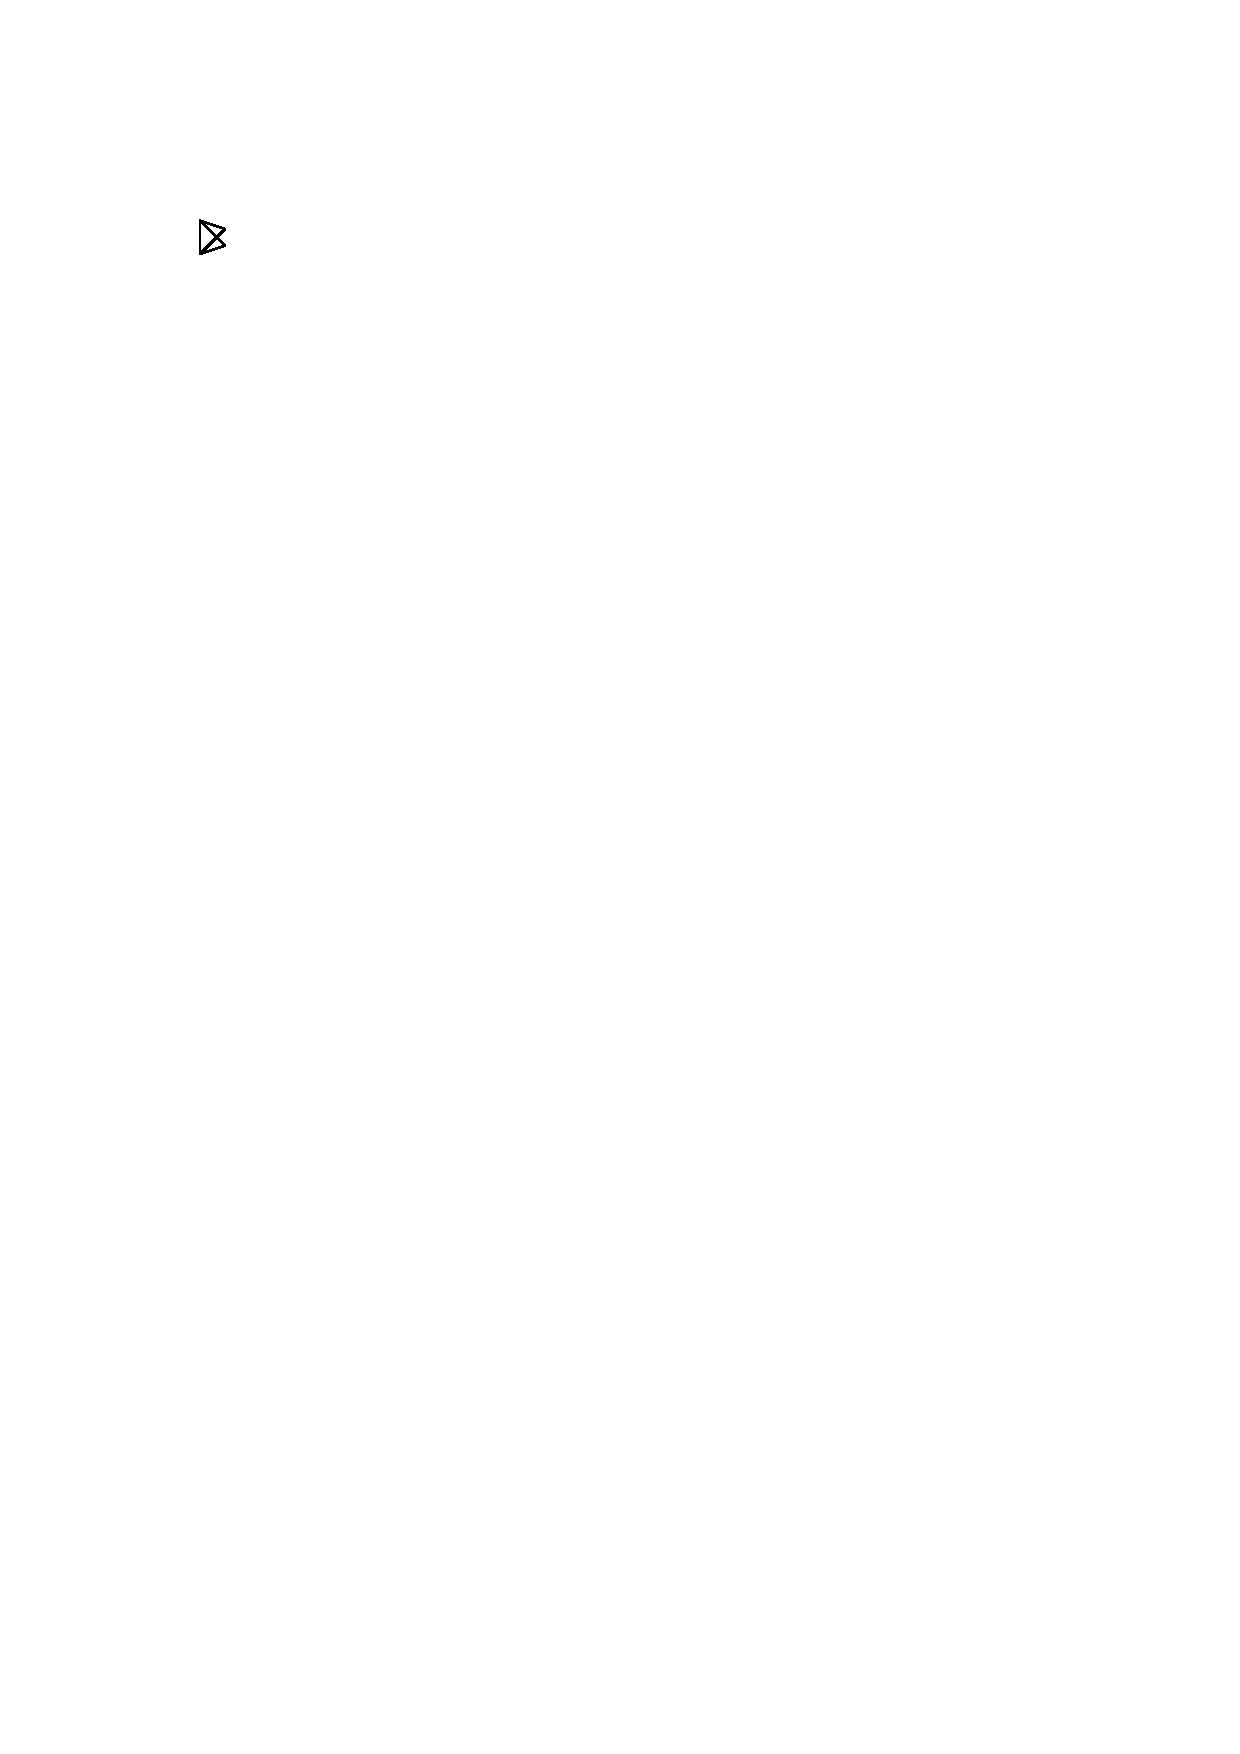
\includegraphics[height=1.6ex]{figs/triangles-edge-1}}}
\newcommand{\mariposa}{\raisebox{-.1ex}{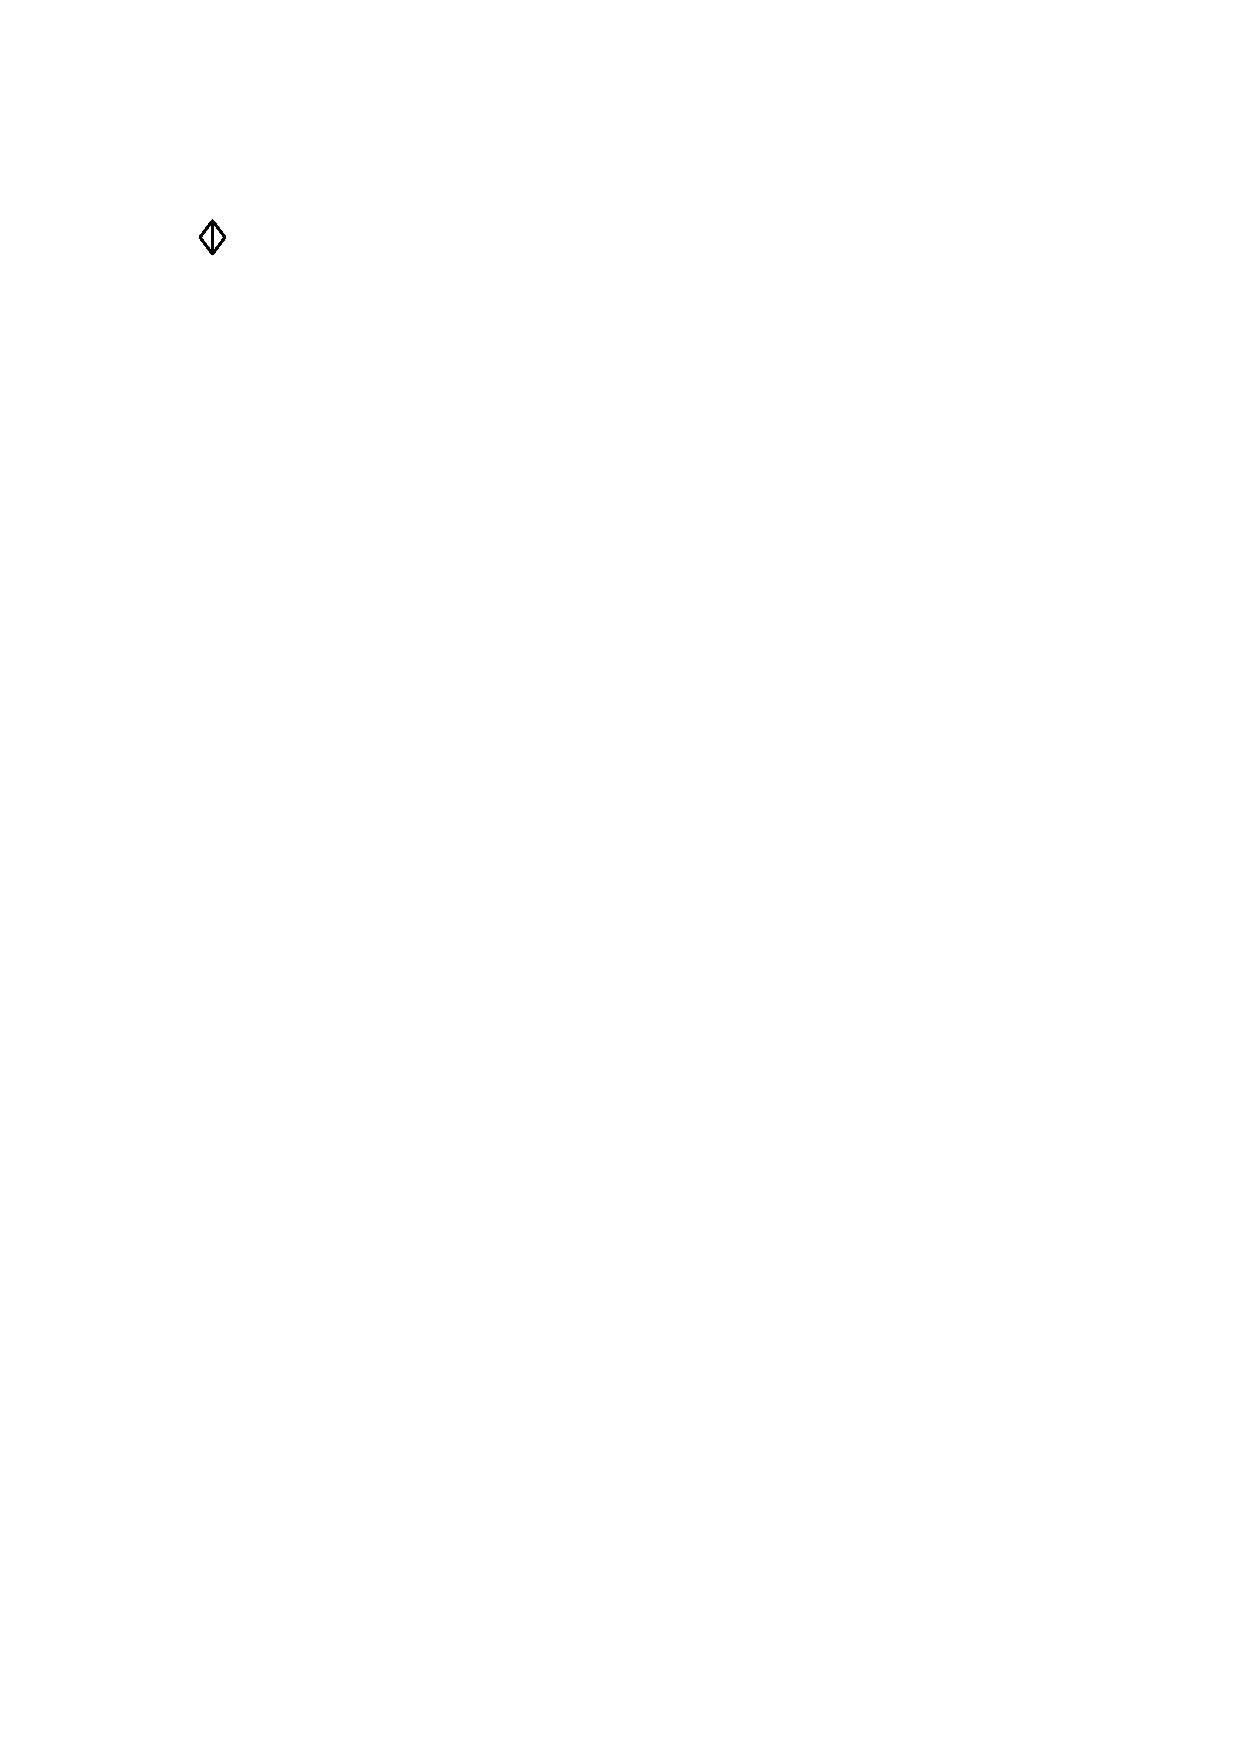
\includegraphics[height=1.6ex]{figs/triangles-edge-2}}}


\newcommand{\bat}{\raisebox{-.1ex}{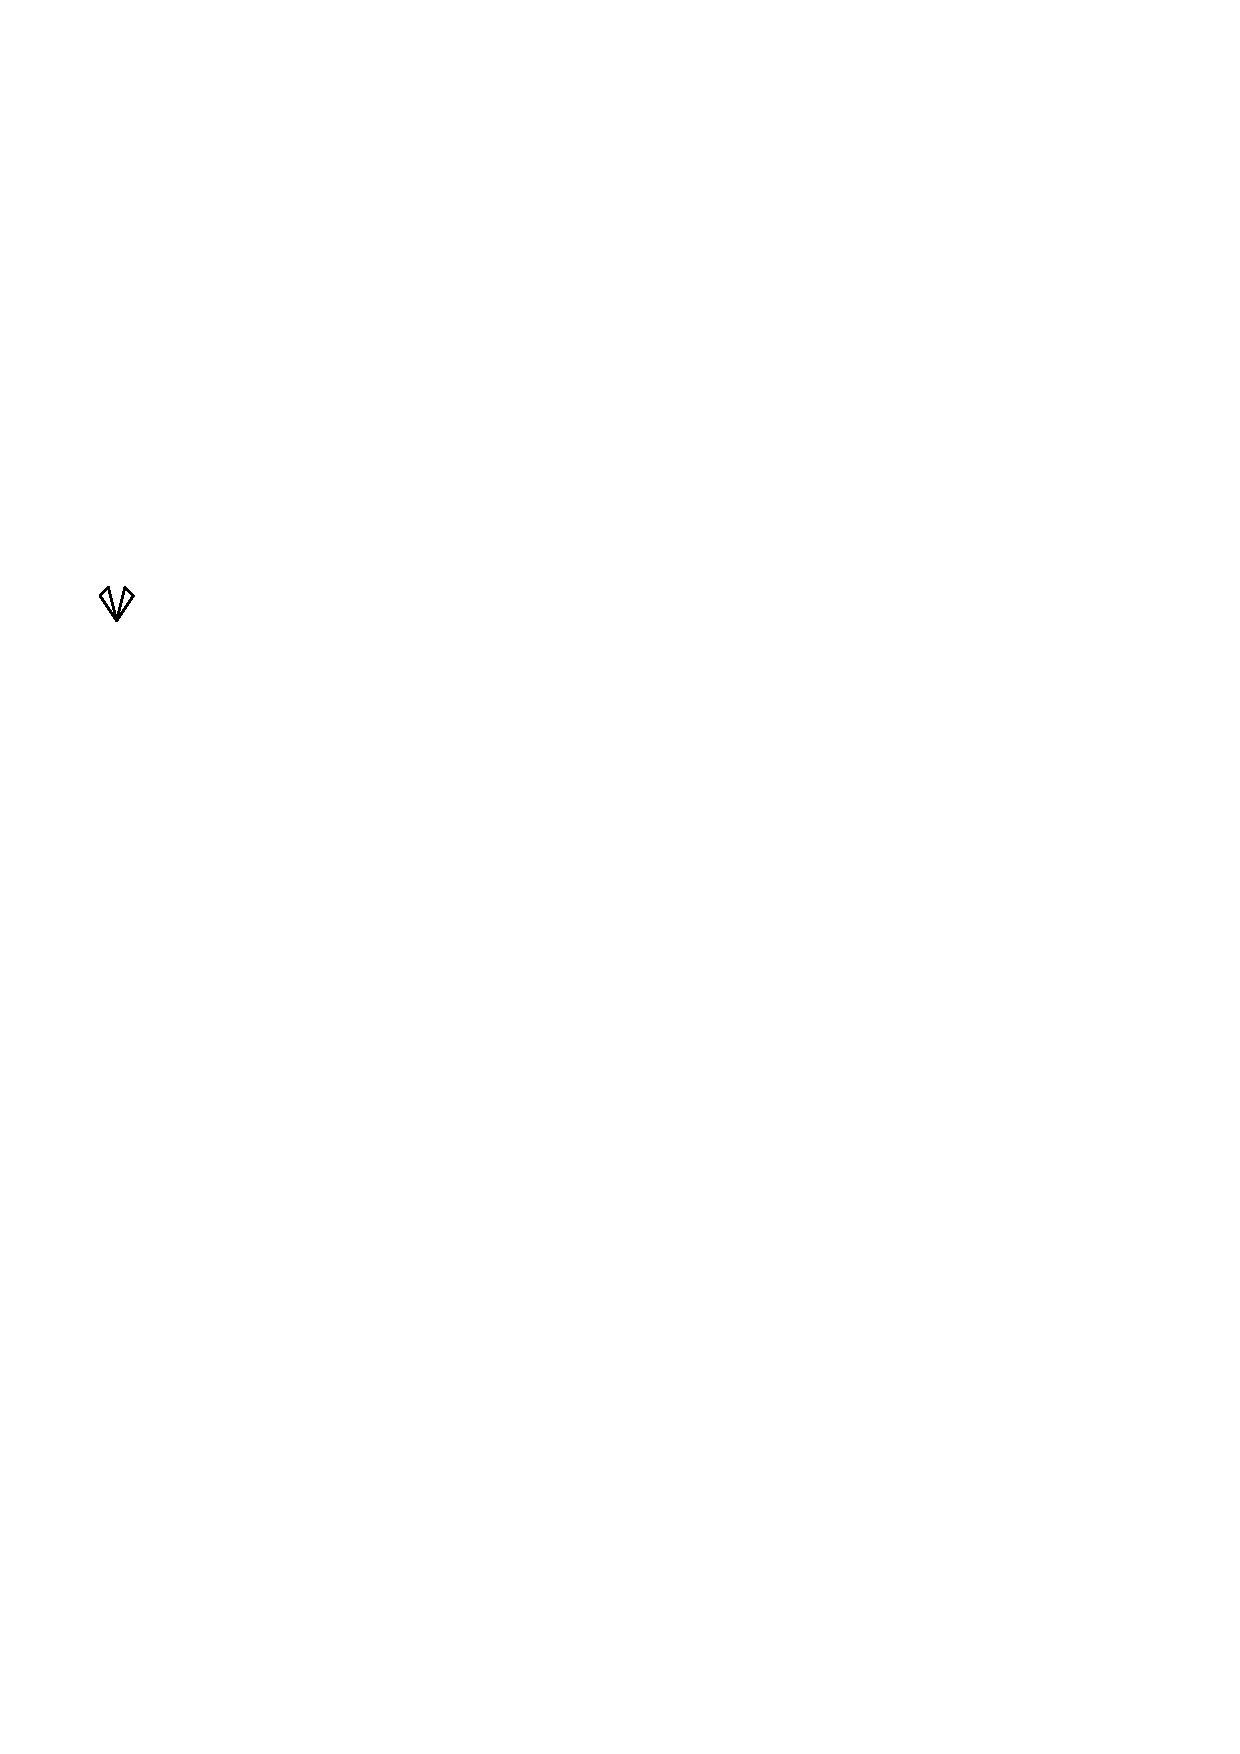
\includegraphics[height=1.6ex]{figs/triangles-vertex-1}}}
\newcommand{\nested}{\raisebox{-.1ex}{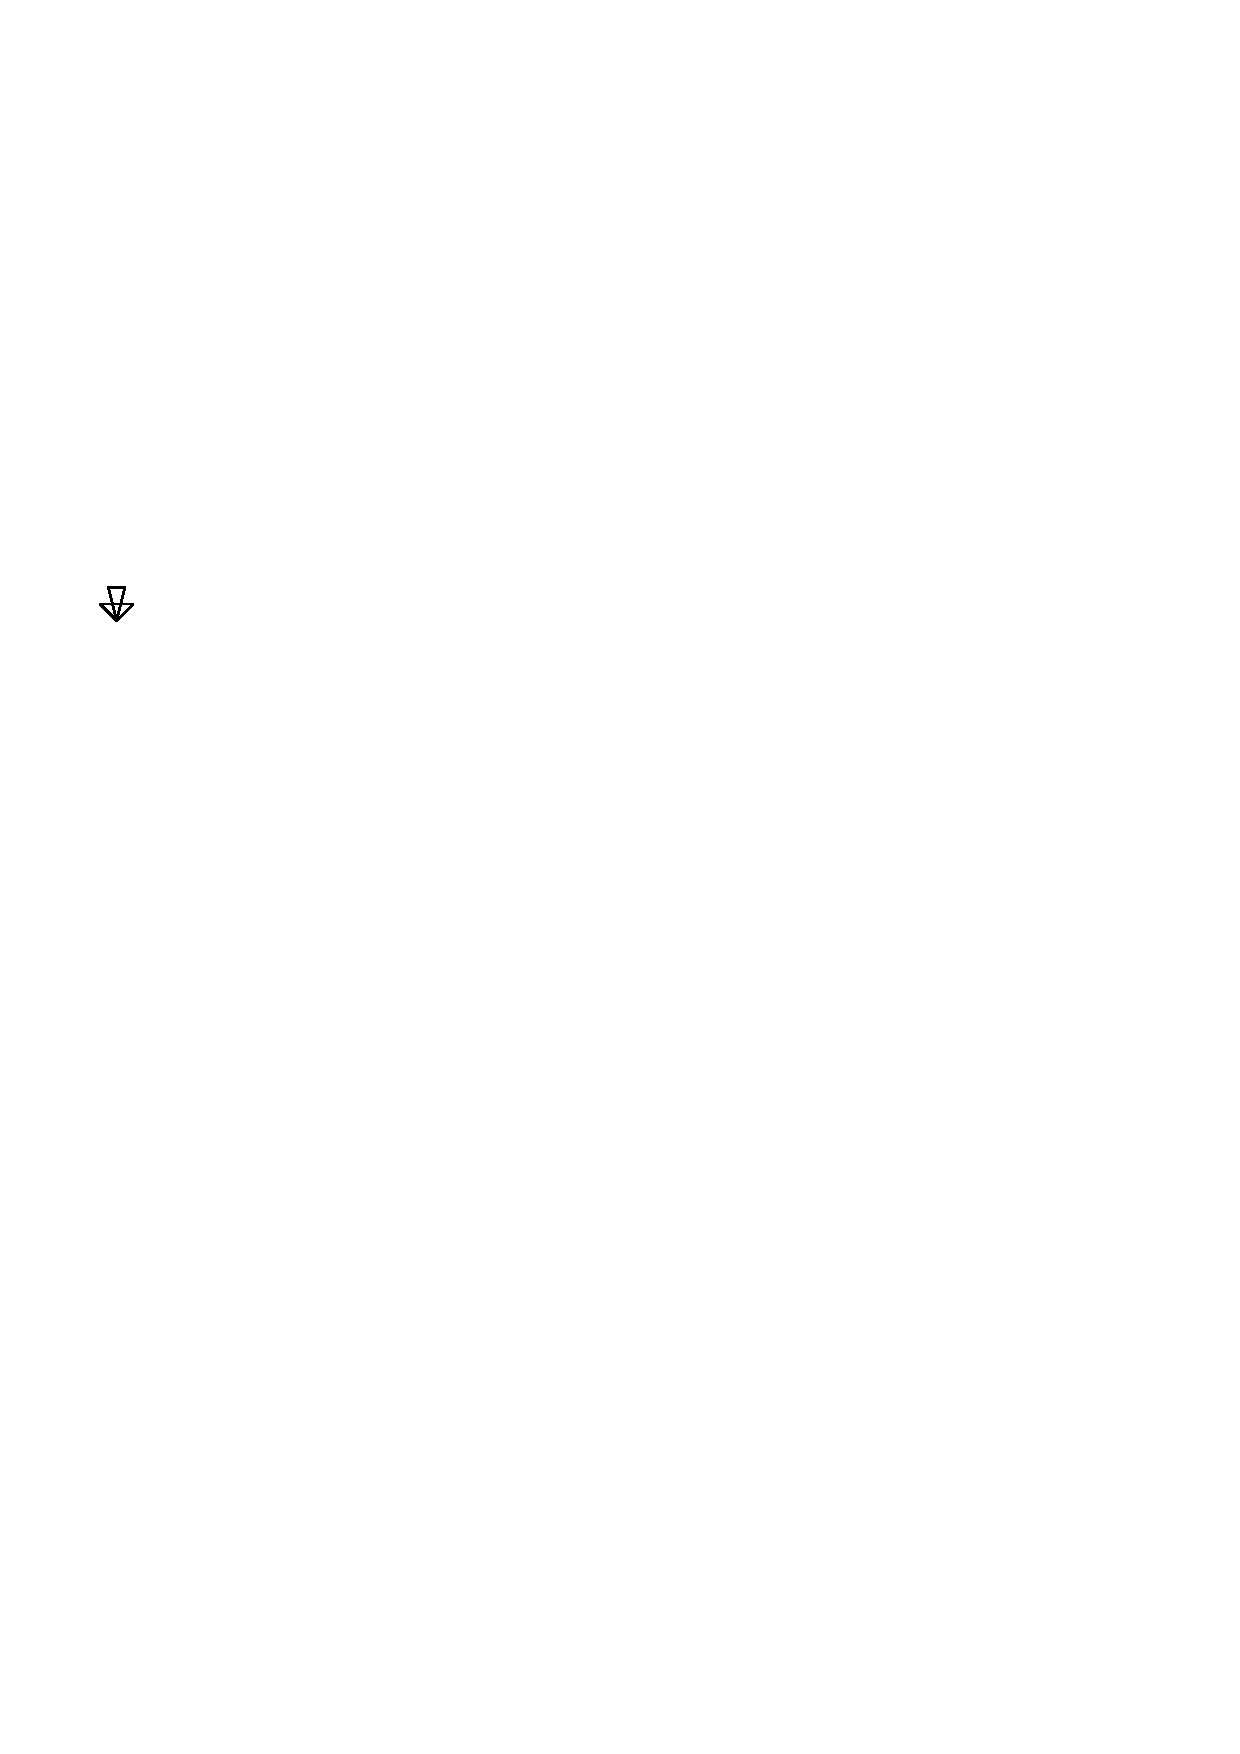
\includegraphics[height=1.6ex]{figs/triangles-vertex-2}}}
\newcommand{\crossing}{\raisebox{-.1ex}{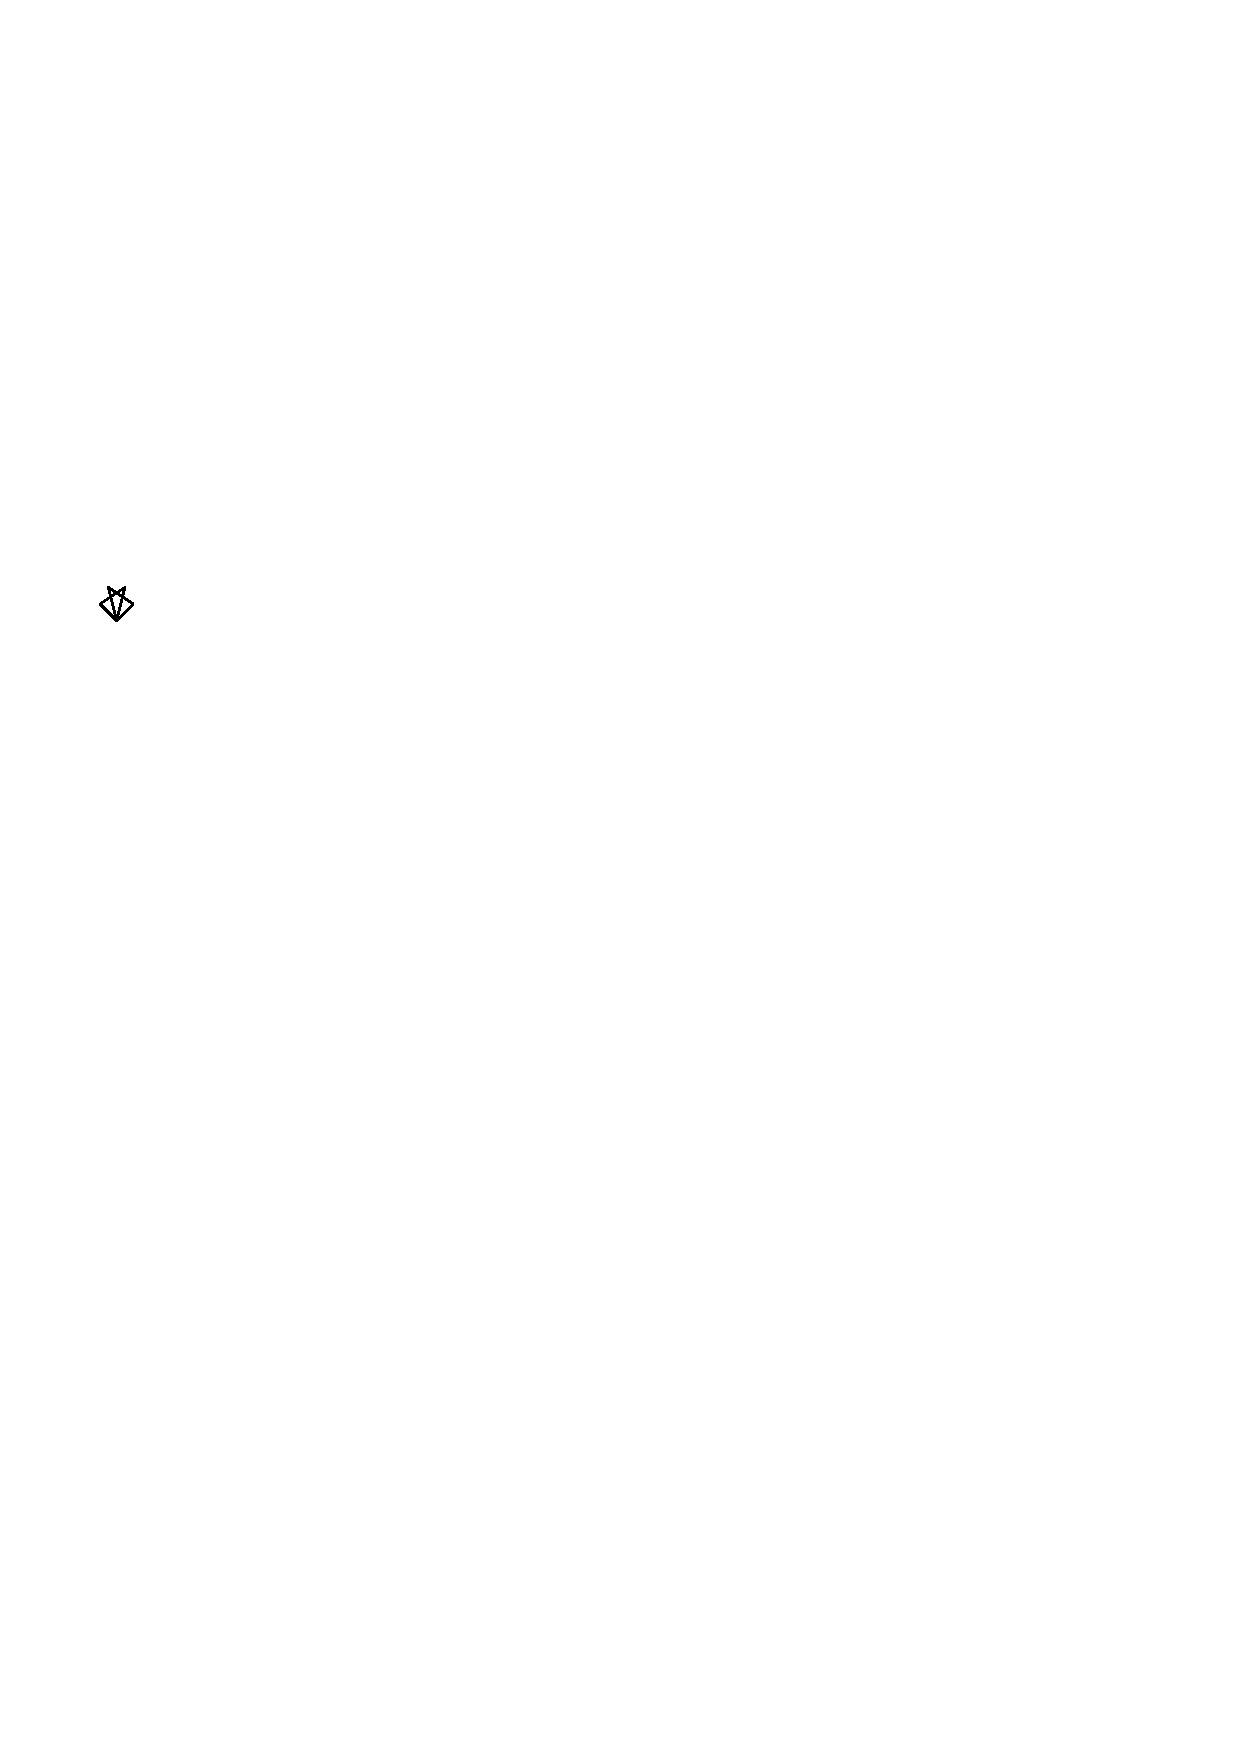
\includegraphics[height=1.6ex]{figs/triangles-vertex-3}}}

\newcommand{\ears}{\raisebox{-.1ex}{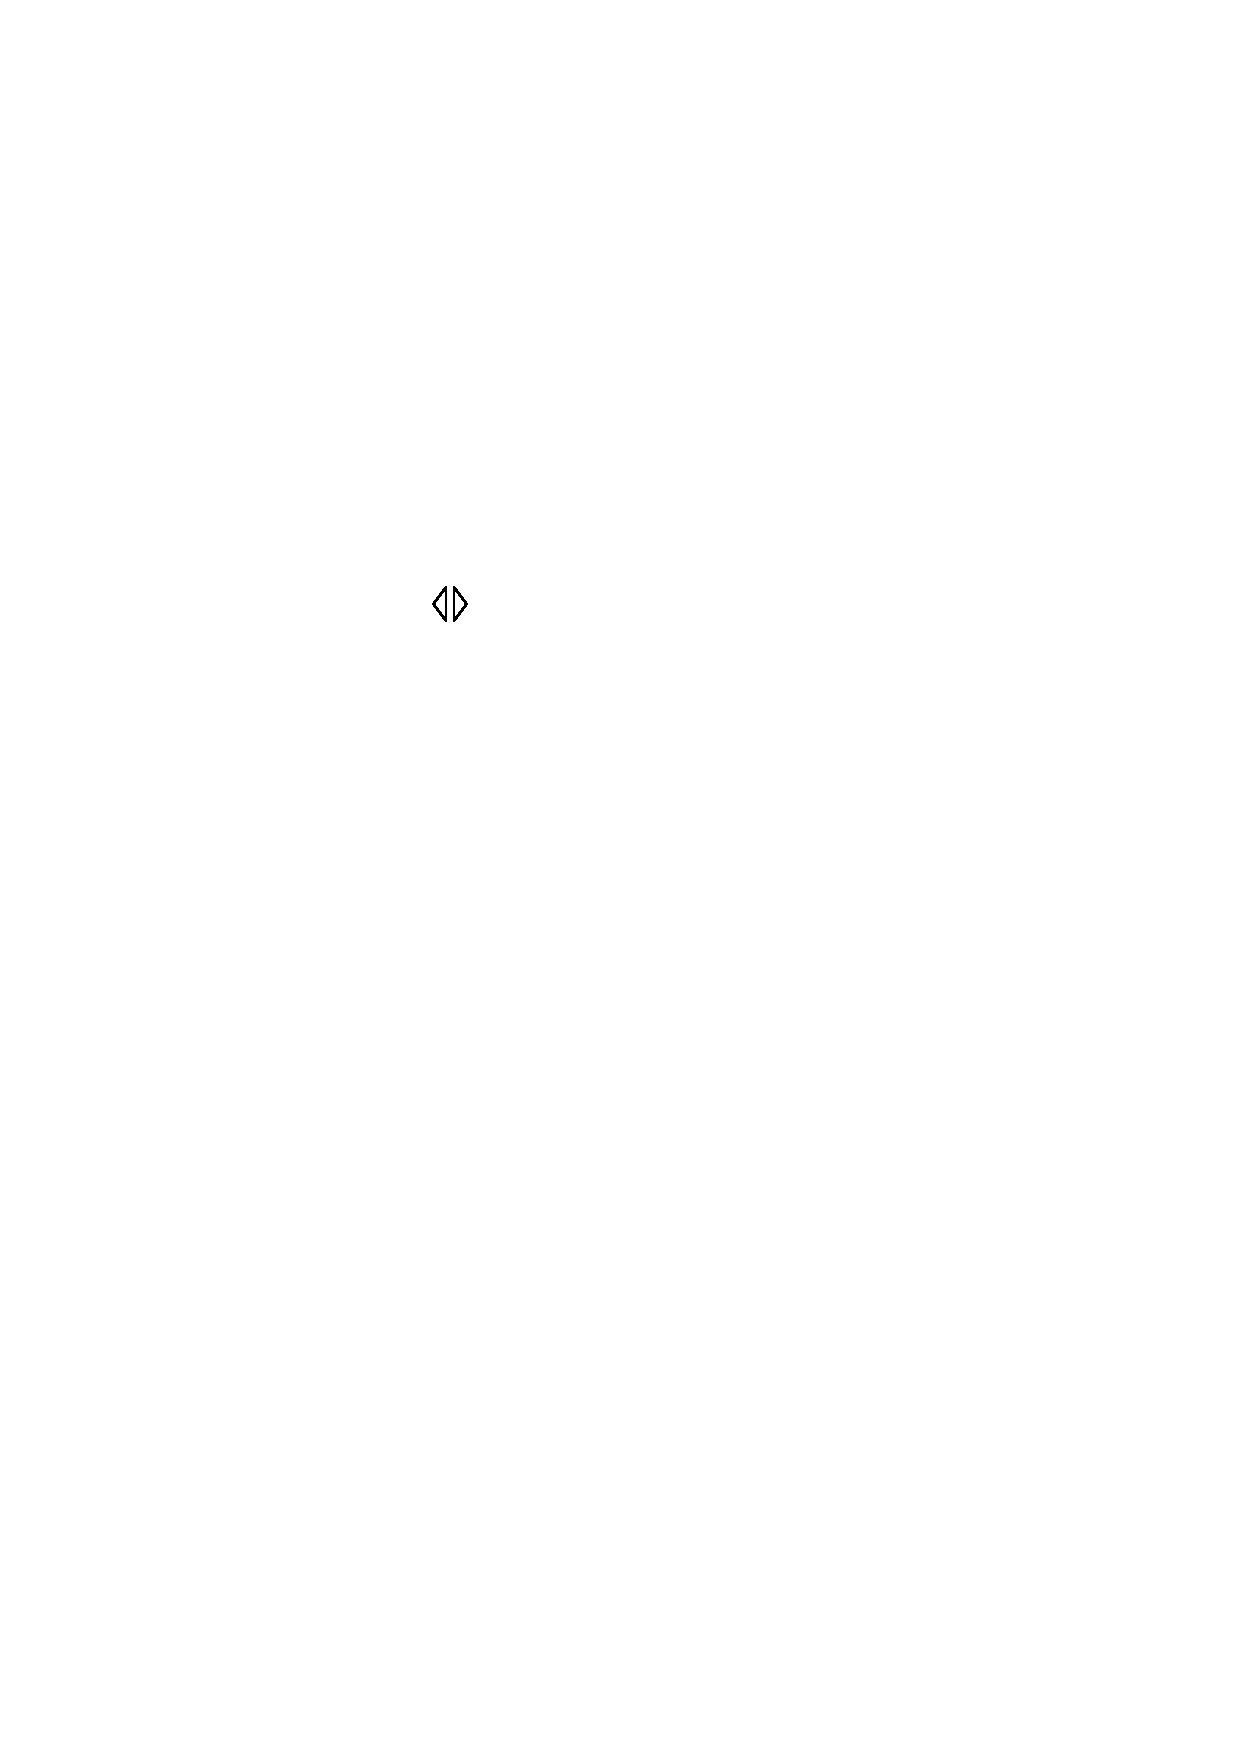
\includegraphics[height=1.6ex]{figs/triangles-disjoint-1}}}
\newcommand{\swords}{\raisebox{-.1ex}{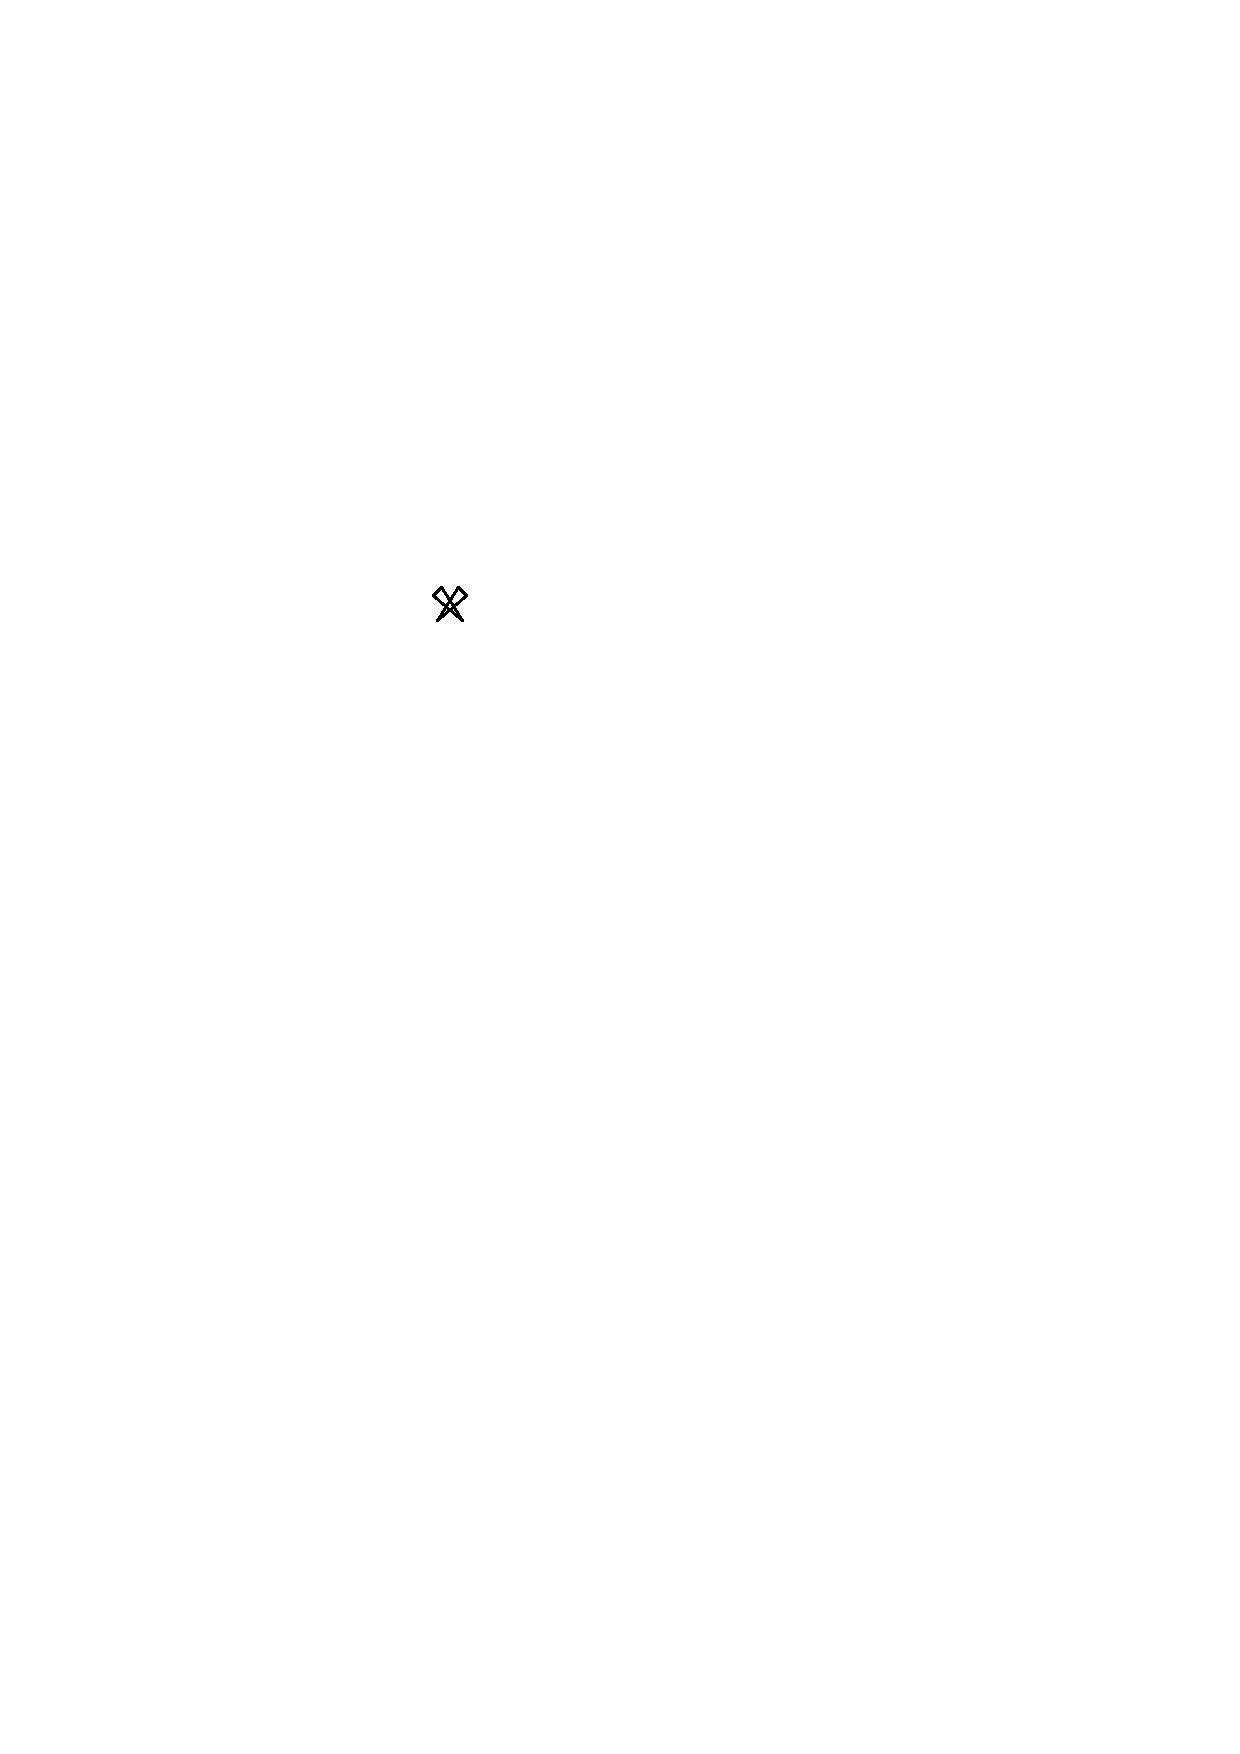
\includegraphics[height=1.6ex]{figs/triangles-disjoint-2}}}
\newcommand{\david}{\raisebox{-.1ex}{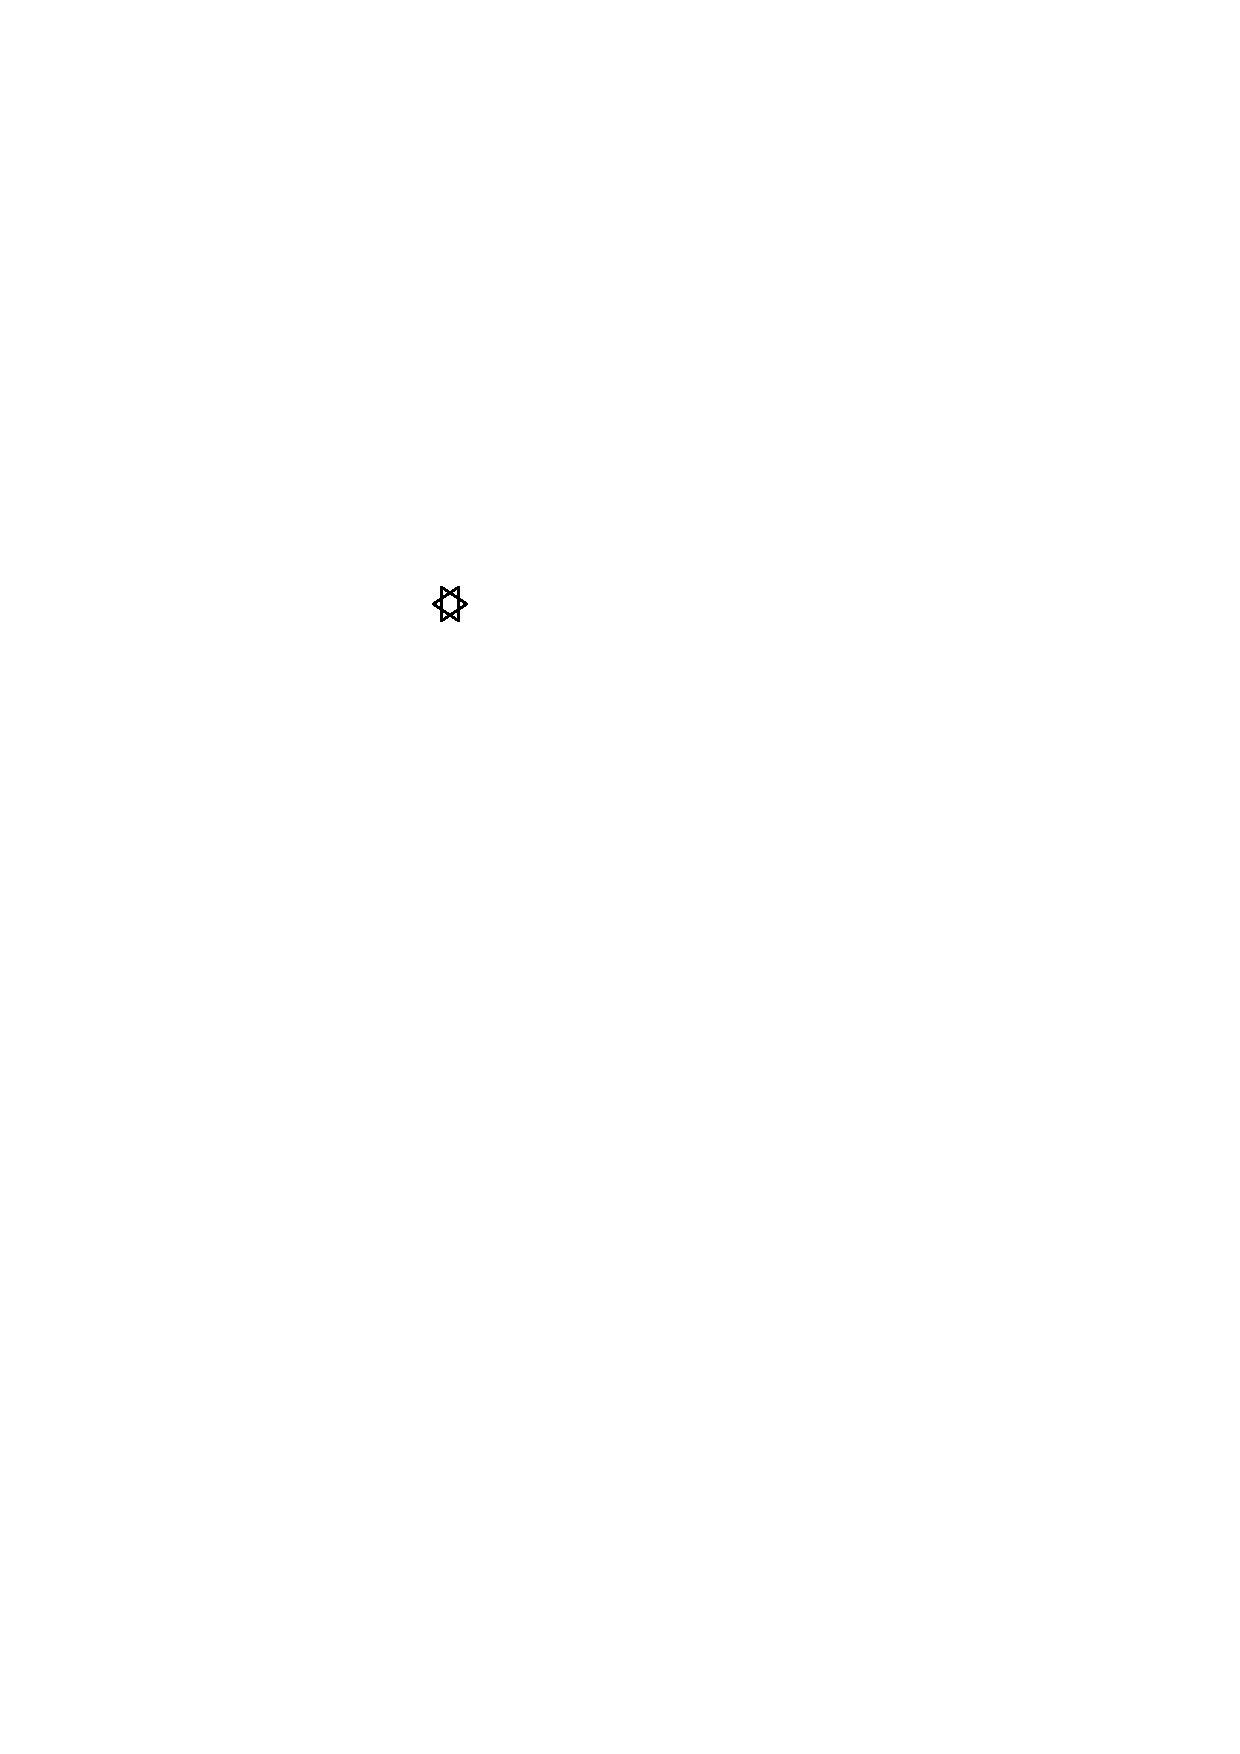
\includegraphics[height=1.6ex]{figs/triangles-disjoint-3}}}

\DeclareMathOperator{\ex}{ex}
\DeclareMathOperator{\on}{\overline{ex}}



%\usepackage{lineno}
%\linenumbers

\pagenumbering{roman}
\begin{document}
\begin{titlepage}
\maketitle

\begin{abstract}
  We study the following family of problems: Given a set of $n$ points
  in convex position, what is the maximum number triangles one can create
  having these points as vertices while avoiding certain \emph{forbidden
  configurations}.  As forbidden configurations we consider all 8 ways
  in which a pair of triangles in such a point set can interact.
\end{abstract}

\end{titlepage}

\tableofcontents

\newpage

\section{Introduction}
\pagenumbering{arabic}

Let $t_1$ and $t_2$ be a pair of distinct triangles whose (4--6) vertices
are in convex position.  There are 8 combinatorially distinct ways that
these triangle can interact:  2 ways in which the triangles can share
an edge (\taco\ and \mariposa), 3 ways in which the triangles can share a
single vertex (\bat, \nested, and \crossing), and 3 ways in which
the triangles can have no vertices in common (\ears, \swords,
and \david).

We consider the following class of problems:  Given a set, $X$,
of combinatorial configurations of pairs of triangles, what is the
largest set, $S$, of triangles one can create whose vertices are $n$
points in convex position, and such that no pair of triangles in $S$
forms a configuration in $X$.  We call the size of this set $\ex(n,X)$.
For example, 
\begin{equation}
    \ex(n,\{\taco,\nested,\crossing,\swords,\david\}) = n-2 \enspace .
\end{equation}
This is because the set $X=\{\taco,\nested,\crossing,\swords,\david\}$
forbids any form of crossings between the edges of triangles. Thus, the
maximum number of triangles we can have while avoiding $X$ is the number
of triangles in a triangulation of a convex $n$-gon, i.e., $n-2$. 

\subsection{Previous Work}

Since there are eight possible forbidden configurations, there are
$2^8=256$ sets, $X$ for which we can study $\ex(n,X)$.  Some of these sets
have been previously studied.  Bra\ss, Rote, and Swanepoel used bounds on
the set $X=\{\ears,\swords,\bat,\nested\}$ to solve an Erd\H{o}s problem
on the maximum number of maximum area/perimeter triangles determined
by a point set. Bra\ss\ \cite{brass:turan} later began a systematic
study in which he gave tight bounds for all singleton $X$ and all
pairs of configurations in which two triangles share a single vertex.
These previous results are listed in \tabref{previous}.

%One
%of the results in this paper is that nearly the same bound holds even
%if we allow the $\swords$ and $\david$ configuration. In particular,
%our \thmref{blech} shows that $\ex(n,\{\taco,\nested,\crossing\}) \in
%O(n\log n)$.
%
%Sometimes it is more natural to describe the allowable configurations than the forbidden configurations. For this, we use the notation 
%\[
%   \on(n,X) = \ex(n,\{\taco,\mariposa,\bat,\nested,\crossing,
%                       \ears,\swords,\david\} \setminus X) \enspace .
%\]
%

\begin{table}
\begin{center}
\begin{tabular}{m{.55\textwidth}m{.4\textwidth}}
  \hline
  \textbf{Result} & \textbf{Ref.} \\ \hline\hline
  $\ex(n,\{\mariposa\})\in \Theta(n^3)$ \newline
  $\ex(n,\{\taco\})\in \Theta(n^2)$ & \cite{brass:turan} \\
  \hline
  $\ex(n,\{\bat\})\in \Theta(n^3)$ \newline
  $\ex(n,\{\nested\})\in \Theta(n^2)$ \newline
  $\ex(n,\{\crossing\})\in \Theta(n^2)$ & \cite{brass:turan} \\
  \hline
  $\ex(n,\{\ears\})\in \Theta(n^3)$ \newline
  $\ex(n,\{\swords\})\in \Theta(n^2)$ \newline
  $\ex(n,\{\david\})\in \Theta(n^2)$ & \cite{brass:turan} \\
  \hline
  $\ex(n,\{\bat,\nested\})\in \Theta(n^2)$ \newline 
  $\ex(n,\{\nested,\crossing\})\in \Theta(n^2)$ \newline
  $\ex(n,\{\bat,\crossing\})\in \Theta(n^2)$ & \cite{brass:turan} \\
  \hline
  $\ex(n,\{\ears,\swords,\bat,\nested\}) = n$ \newline
  $\on(n,\{\taco,\mariposa,\david,\crossing\}) = n$
    & \cite{brass.rote.ea:triangles} \\
  \hline
  $\ex(n,\{\bat,\nested,\crossing\}) \in \Theta(n)$ \newline
  $\ex(n,\{\taco,\mariposa\}) \in \Theta(n^2)$ \newline 
  $\ex(n,\{\ears,\swords,\david\}) \in \Theta(n^2)$ & from hypergraphs \\ \hline
  \end{tabular}
\end{center}
\caption{Known results on $\ex(n,X)$ for different sets $X$.}
\tablabel{previous}
\end{table}


%\begin{tabular}{llll}\hline
%  $\ex(n,\taco,\bat)$ & \multicolumn{2}{c}{$\Theta(n^2)$} & \thmref{taco-bat} \\
%  $\ex(n,\taco,\nested)$ & $\Omega(n^{1.549})$ & $O(n^2)$ & [various] \\
%  $\ex(n,\taco,\nested,\david)$ & $\Omega(n)$ & $O(n\log n)$ & \thmref{taco-nested-david} \\
%  $\ex(n,\taco,\crossing)$ & & & \\
%  $\ex(n,\taco,\ears)$ & \multicolumn{2}{c}{$\Theta(n^2)$} & \thmref{taco-ears} \\
%  $\ex(n,\taco,\david)$ & \multicolumn{2}{c}{$\Theta(n^2)$} & \thmref{taco-david} \\
%  $\ex(n,\taco,\swords)$ & $\Omega(n)$ & $O(n\log n)$ & \thmref{taco-swords} \\
%  $\ex(n,\bat,\nested)$ & \multicolumn{2}{c}{$\Theta(n^2$)} & \cite{brass:turan} \\
%  $\ex(n,\bat,\crossing)$ & \multicolumn{2}{c}{$\Theta(n^2$)} & \cite{brass:turan} \\
%  $\ex(n,\bat,\ears)$ & & & \\
%  $\ex(n,\bat,\swords)$ & \multicolumn{2}{c}{$\Theta(n^2$)} & \thmref{bat-swords} \\
%  $\ex(n,\bat,\david)$ & & & \\
%  $\ex(n,\nested,\crossing)$ & \multicolumn{2}{c}{$\Theta(n^2$)} & \cite{brass:turan} \\
%  $\ex(n,\nested,\ears)$ & & & \\
%  $\ex(n,\nested,\swords)$ & $\Omega(n)$ & $O(n\log n)$ & \thmref{nested-swords} \\
%  $\ex(n,\nested,\david)$ & & & \\
%  $\ex(n,\crossing,\ears)$ & & & \\
%  $\ex(n,\crossing,\swords)$ & $\Omega(n)$ & $O(n\log n)$ & \thmref{crossing-swords} \\$\ex(n,\crossing,\david)$ & & & \\
%  $\ex(n,\ears,\swords)$ & \multicolumn{2}{c}{$\Theta(n^2$)} & \thmref{swords-ears-david} \\
%  $\ex(n,\ears,\david)$ & \multicolumn{2}{c}{$\Theta(n^2$)} & \thmref{swords-ears-david} \\
%  $\ex(n,\swords,\david)$ & \multicolumn{2}{c}{$\Theta(n^2$)} & \thmref{swords-ears-david} \\
%\\ \hline
%\end{tabular}
%

\subsection{New Results}

In the current paper, we determine, up to a logarithmic factor, the
asymptotics of $\ex(n,X)$ for 248 sets $X$.  These results are shown
in \tabref{bigtable}.  Each entry in this table presents the asymptotic
behaviour of $\ex(n,X)$ for the set $X$ obtained as the union of the
row and column label.  The configuration $\mariposa$ is ommitted since
a simple argument (\lemref{xcup}) shows that its inclusion in $X$
does not change $\ex(n,X)$ by more than a constant factor. For the
remaining 8 sets, we have determined that the asymptotics are all the
same and are equivalent to a problem that appears in various contexts
and under different names, including monotone matrices, tripod packing,
and 2-comparable triples. We discuss this problem and its rich history
in \secref{tripods}.

\begin{table}
  \begin{center}
    \input{bounds.tex}
  \end{center}
  \caption{New and previous bounds for $\ex(n,X)$.}
  \tablabel{bigtable}
\end{table}

\section{Points of View and Easy Results}

In this section we present an easy result that cuts our work in half
and we describe different variants of the problem, some of which are
easier to work with.  

\subsection{Edge-Sharing Non-Overlapping Triangles are Irrelevant}

The following lemma shows that including the $\mariposa$ confguration in
the set $X$ of forbidden configurations has no effect on the asymptotics
of $\ex(n,X)$.

\begin{lem}\lemlabel{xcup}
   For any $X$, $\ex(n,X\cup\{\mariposa\}) \ge \ex(n,X)/8$.
\end{lem}

\begin{proof}
  Let $S$ be a set of triangles that achieves $\ex(n,X)$. For each pair
  of vertices $u$ and $w$ independently and uniformly choose a direction
  $\overrightarrow{uw}$ or $\overleftarrow{uw}$.  We then obtain a set
  $S'\subseteq S$ by removing any triangle that has a directed edge for
  which the triangle is to the left of the edge.  Observe that the set
  $S'$ does not contain a $\mariposa$ configuration.

  For any particular triangle $t\in S$, the probability that $t\in S'$
  is exactly $1/8$ since each of $t$'s three edges must be directed
  clockwise and edge directions are chosen independently.  By linearity of
  expectation, $\E[|S'|]=|S|/8=\ex(n,X)/8$.  We conclude therefore that
  there exists some subset $S''\subseteq S$ of size least $\ex(n,X)/8$
  that does not contain a $\mariposa$ configuration.  The set $S''$ proves
  that $\ex(n,X\cup\{\mariposa\}) \ge \ex(n,X)/8$.
\end{proof}

\subsection{The Top/Bottom View}

It will be helpful to gain a sense of orientation by considering
a top/bottom variant of $\ex(n,X)$ that is defined as follows (see
\figref{top-bottom}).  Partition the vertices of a convex $n$-gon using
a horizontal line into a \emph{top half} of size $\lceil n/2\rceil$
and a \emph{bottom half} of size $\lfloor n/2\rfloor$.  We define
$\ex'(n,X)$ analogously to $\ex(n,X)$ except that we only count triangles
having one vertex in the bottom half and two vertices in the top half.
When studying $\ex'$, each triangle we count has a naturally defined
\emph{bottom vertex} in the bottom half and a \emph{left vertex} and
\emph{right vertex}, each in the top half.

\begin{figure}
  \begin{center}
    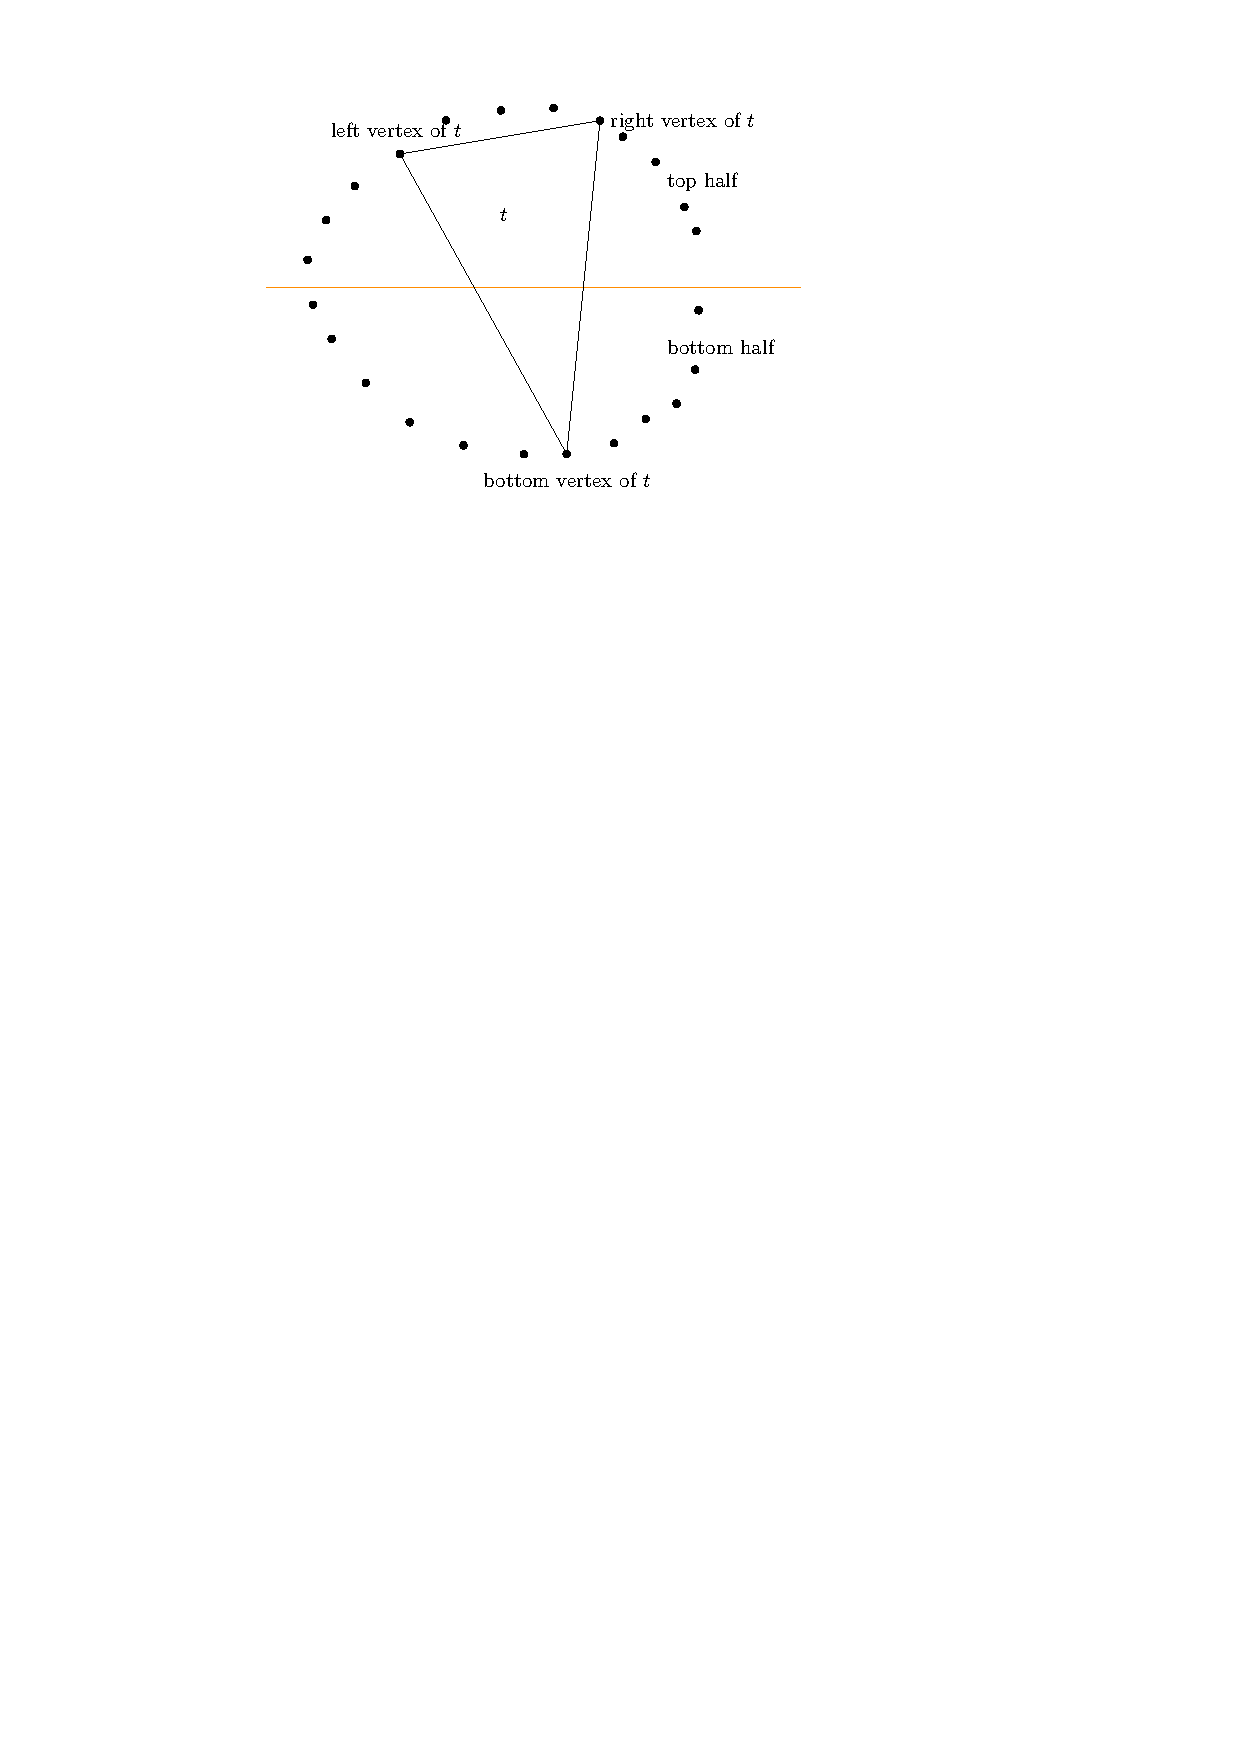
\includegraphics{figs/left-right}
  \end{center}
  \caption{$\ex'$ only counts triangles with two vertices in the top half
     and one vertex in the bottom half.}
  \figlabel{top-bottom}
\end{figure}

Clearly $\ex(n,X)\ge\ex'(n,x)$.  The following lemma shows that, without
losing much precision, we can also upper bound $\ex(n,X)$ by $\ex'(n,X)$.

\begin{lem}\lemlabel{top-bottom}
  If $\ex'(n,X)\in O(n^c)$, then
  \[
     \ex(n,X)\in 
        \begin{cases} 
            O(n^c)     & \text{if $c>1$} \\
            O(n\log n) & \text{if $c=1$}
        \end{cases}
  \]
\end{lem}

\begin{proof}
   Let $S$ be a set of triangles that avoids $X$.  Every triangle in $S$
   is of one of the following types:
   \begin{enumerate}
      \item It has one vertex in the top half and two in the bottom half;
        there are $O(n^{c})$ such triangles.
      \item It has two vertices in the top half and one in the bottom
        half; there are $O(n^{c})$ such triangles.
      \item It has all three vertices in the top half; there are at most
        $\ex(\lceil n/2\rceil,X)$ such triangles.
      \item It has all three vertices in the bottom half; there are at
        most $\ex(\lfloor n/2\rfloor,X)$ such triangles.
   \end{enumerate}
   Thus, we obtain the recurrence inequality:
   \[  \ex(n,X) = O(n^{c}) + \ex(\lceil n/2\rceil,X) + \ex(\lfloor n/2\rfloor,X) \]
   which resolves to $O(n^c)$ for $c>1$ and $O(n\log n)$ for $c=1$.
\end{proof}


\subsection{The Dot-Puzzle View}

The top-bottom version of the problem gives us a sense of orientation,
but it is still difficult to visualize the sets of triangles obtained
this way. Next, we show that there is a corresponding puzzle that is
easy to visualize.  Refer to \figref{point-view}.  

In this puzzle, we are given $\binom{n}{2}$ points,
\[
    Q = \{(x,y): y\in\{1,\ldots,n-1\}, x\in\{y+1,\ldots,n-1\} \} \enspace .
\]
These points model the top/bottom view on a convex $2n$-gon, where the
point $(x,y)$ represents a triangle whose vertices are some point on
the bottom and the $x$th and $y$th points on the top, where the top
vertices are labelled $1,\ldots,n$ from left to right.

\begin{figure}
   \begin{center}
      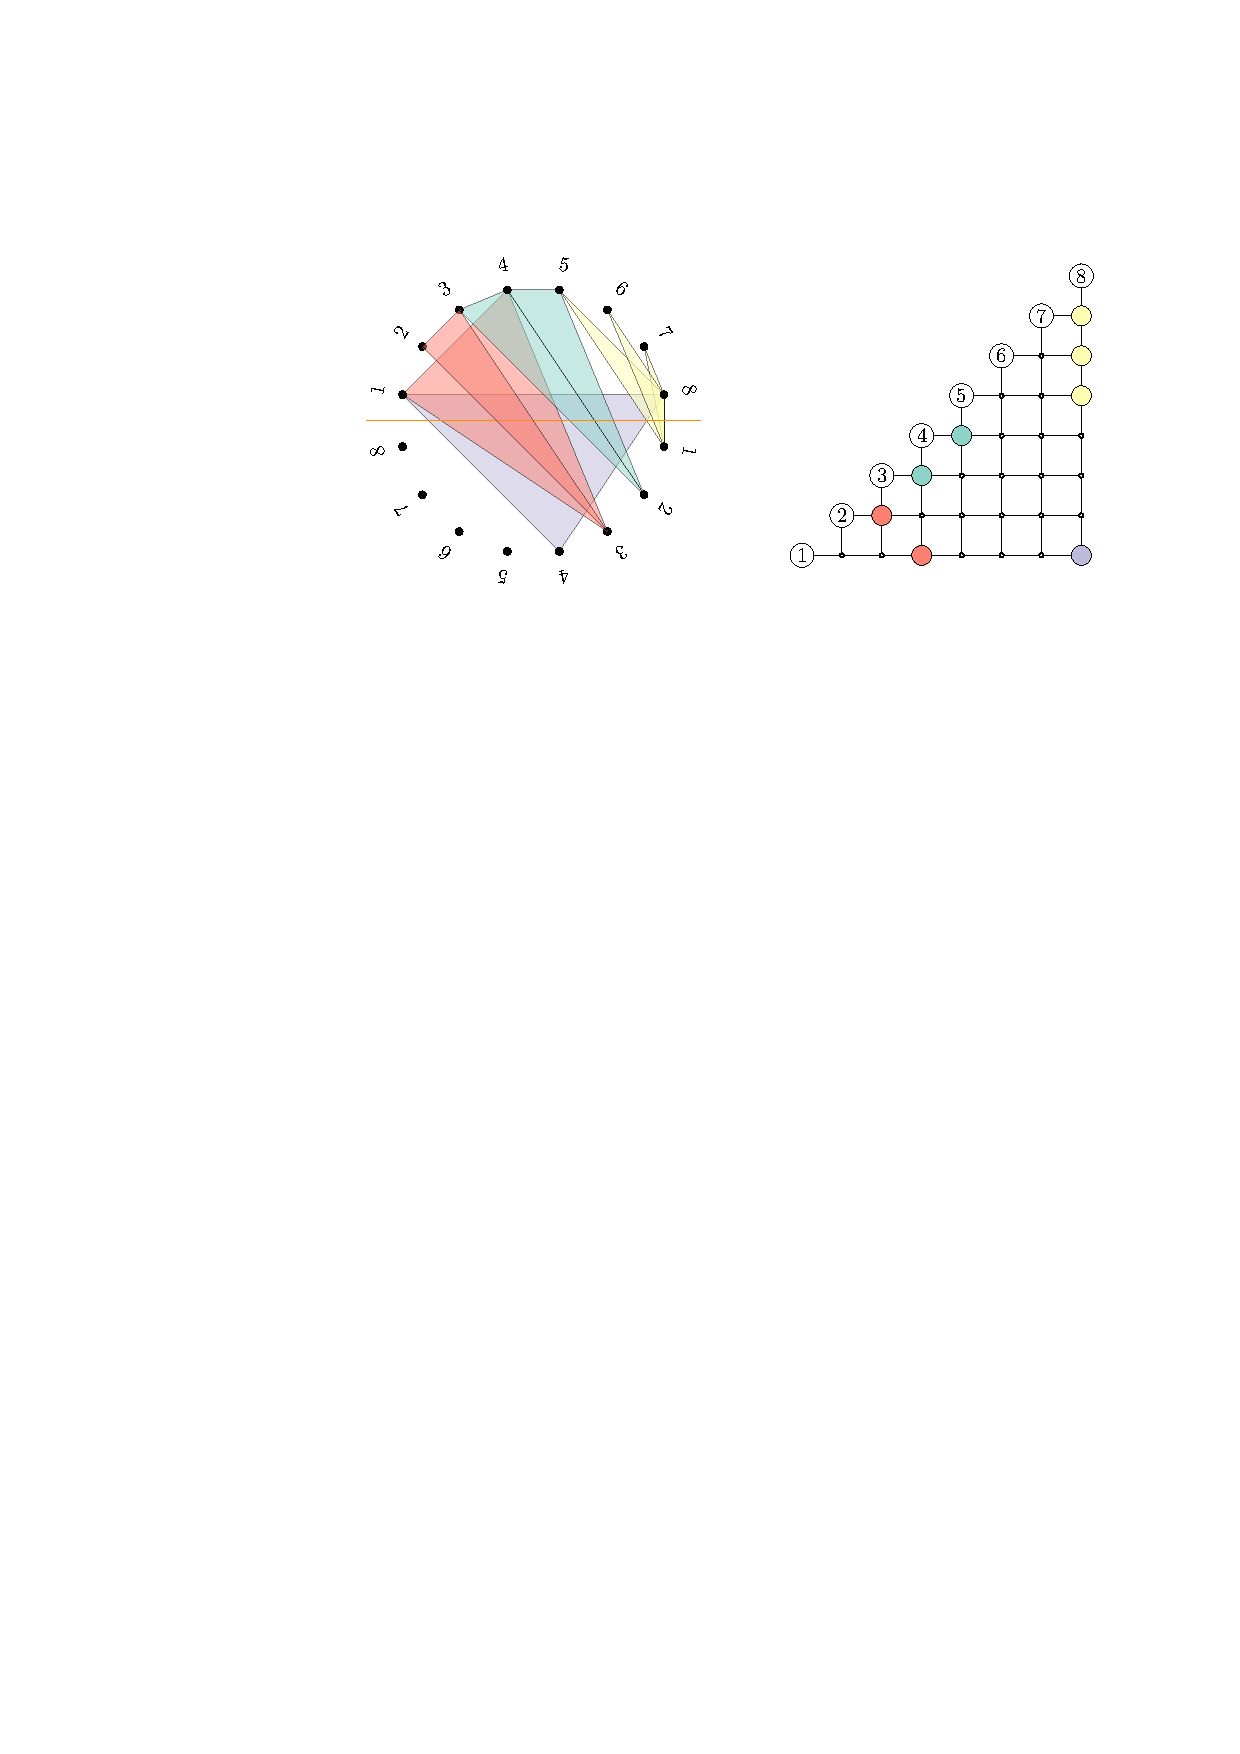
\includegraphics{figs/point-view}
   \end{center}
   \caption{The Dot-Puzzle View of the Top/Bottom View. In this example,
     four rounds of the Dot-Puzzle have been played.}
   \figlabel{point-view}
\end{figure}

The dot-puzzle proceeds in $n$ rounds and during the $i$th round, the
player selects a set $Q_i\subseteq Q$ subject to certain constraints
that depend on the points selected in rounds $1,\ldots,i-1$.  In the
top/bottom view, the $i$th round determines which pairs of top vertices
form a triangle with the $i$th bottom vertex, where the bottom
vertices are labelled $1,\ldots,n$ from right to left.  

Of course, the constraints on which points can be selected during
round $i$ depend on the set of forbidden configurations and the set
$\bigcup_{j=1}^{i-1} Q_i$ of points played during previous rounds.
By proving bounds on $\sum_{i=1}^n |Q_i|$ we obtain bounds on the maximum
number of triangles obtained in the top-bottom view on a set of $2n$
points.

\Figref{forbidden-color}.a shows restrictions on the locations of points
placed during a single round.  It is interpreted as follows:  If the
central point, $p=(x,y)$, is placed during round $i$, and we wish to
avoid some particular configuration, $c$, then we should not place any
points in the parts of the figure that are have label $c$.  For instance,
if we wish to avoid the configuration $c=\taco$ configuration, then we
should not place any points in the same row or column as $p$; such a point
creates a $\taco$ configuration in which the shared edge
joins a bottom vertex to a left (same row) or right (same column) vertex.

\Figref{forbidden-color}.b shows the constraints placed on the locations
of points placed in subsequent rounds.  Its interpretation is similar
\figref{forbidden-color}.a. For example, if we wish to avoid a
$\nested$ configuration and we place the central point, $p$, during round
$i$, then, in every round $j>i$, we should not place any point directly
to the left or directly below $p$.  Any such point creates 
a $\nested$ configuration in which the shared vertex is the left vertex
(to the left of $p$) or the right vertex (below $p$) of both triangles.

%One caveat worth noting is that, unless $\taco$ is a forbidden
%configuration, the same point can be chosen in different rounds.

%\begin{table}
%\begin{center}
%\begin{tabular}{m{1ex}|>{\centering\arraybackslash}m{.45\textwidth}|>{\centering\arraybackslash}m{.45\textwidth}}
%      & killed by $(x,y)$ in later rounds 
%         & killed by $(x,y)$ in current round \\ \hline
%$\mariposa$ & 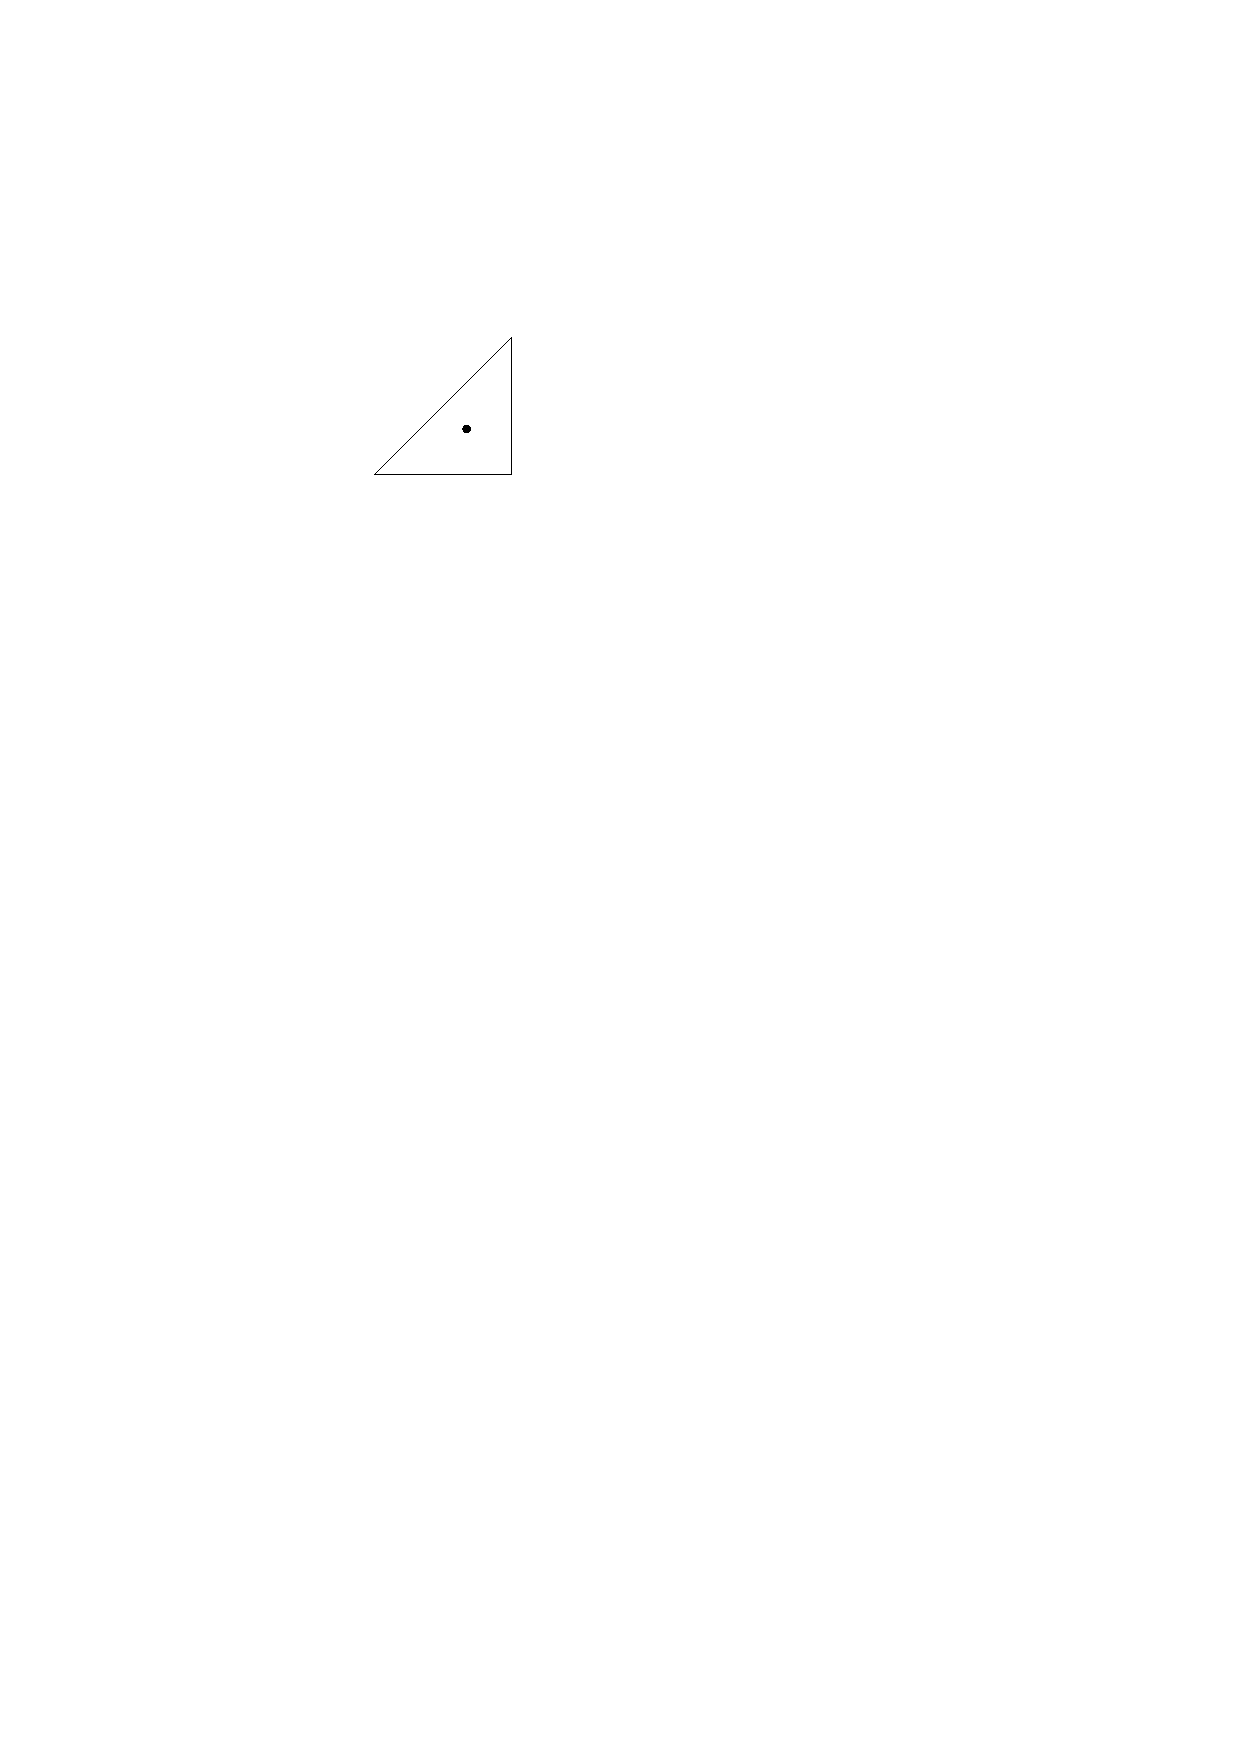
\includegraphics[scale=.8]{figs/killers-1} \break% 
%           $\{\}$  
%         & 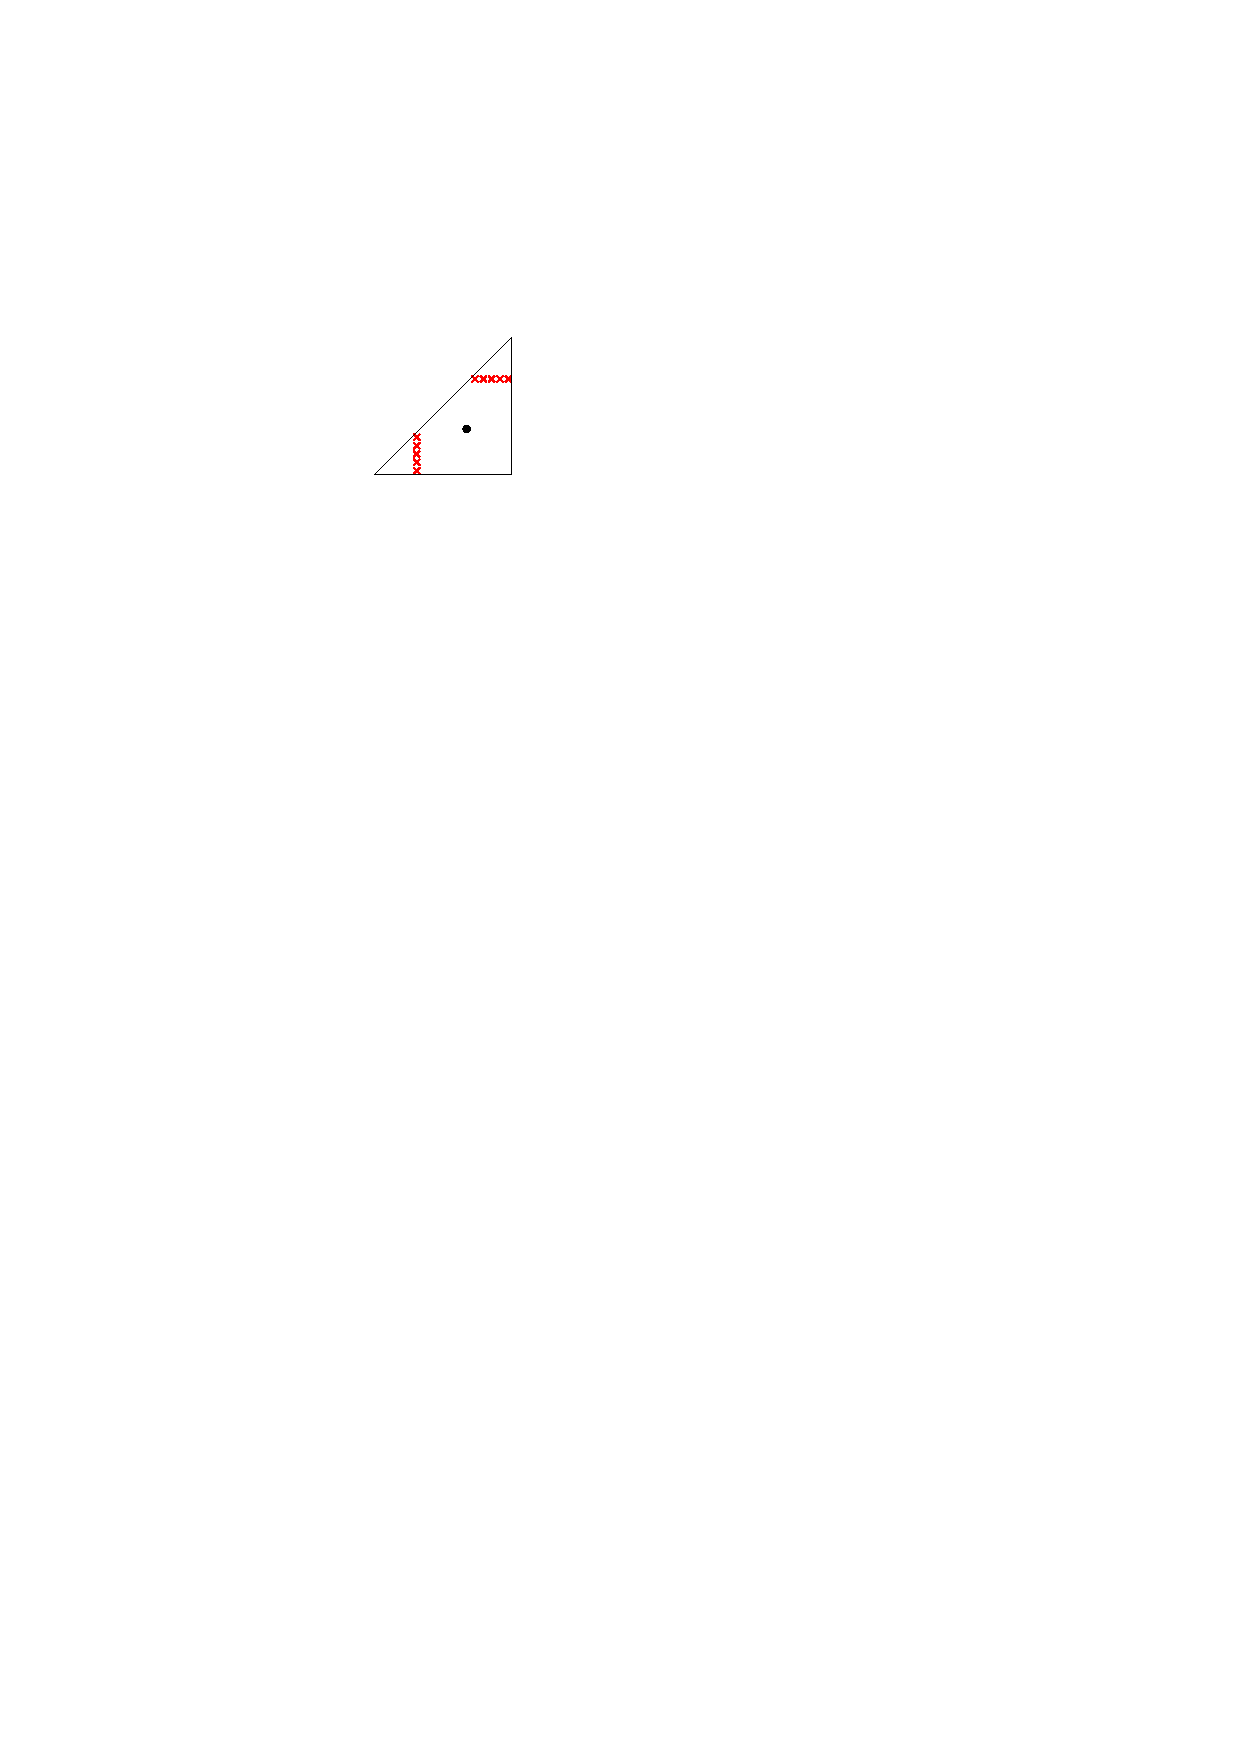
\includegraphics[scale=.8]{figs/killersb-1} \break% 
%           $\{(x',x)\} \cup \{(y,y')\}$ \\ 
%$\taco$ & 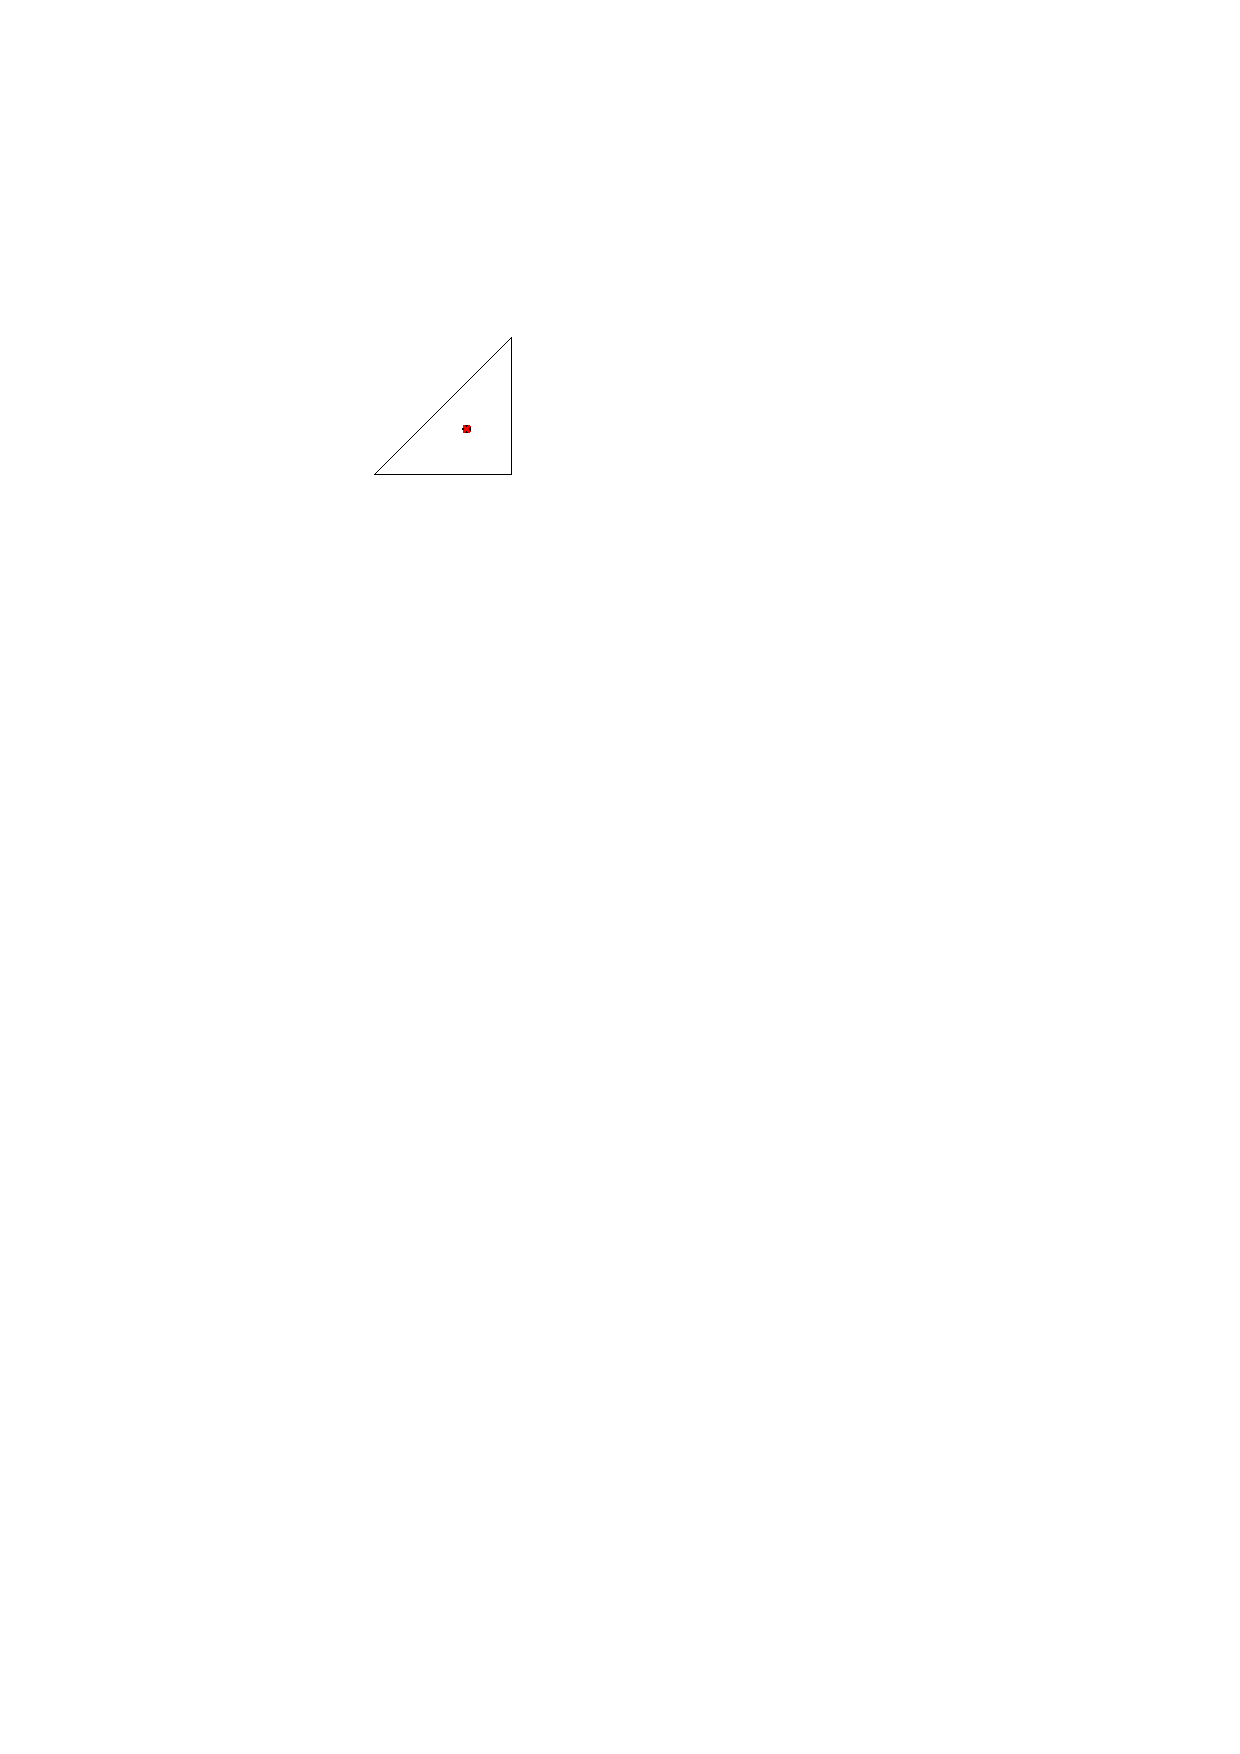
\includegraphics[scale=.8]{figs/killers-2} \break% 
%           $\{(x,y)\}$ 
%         & 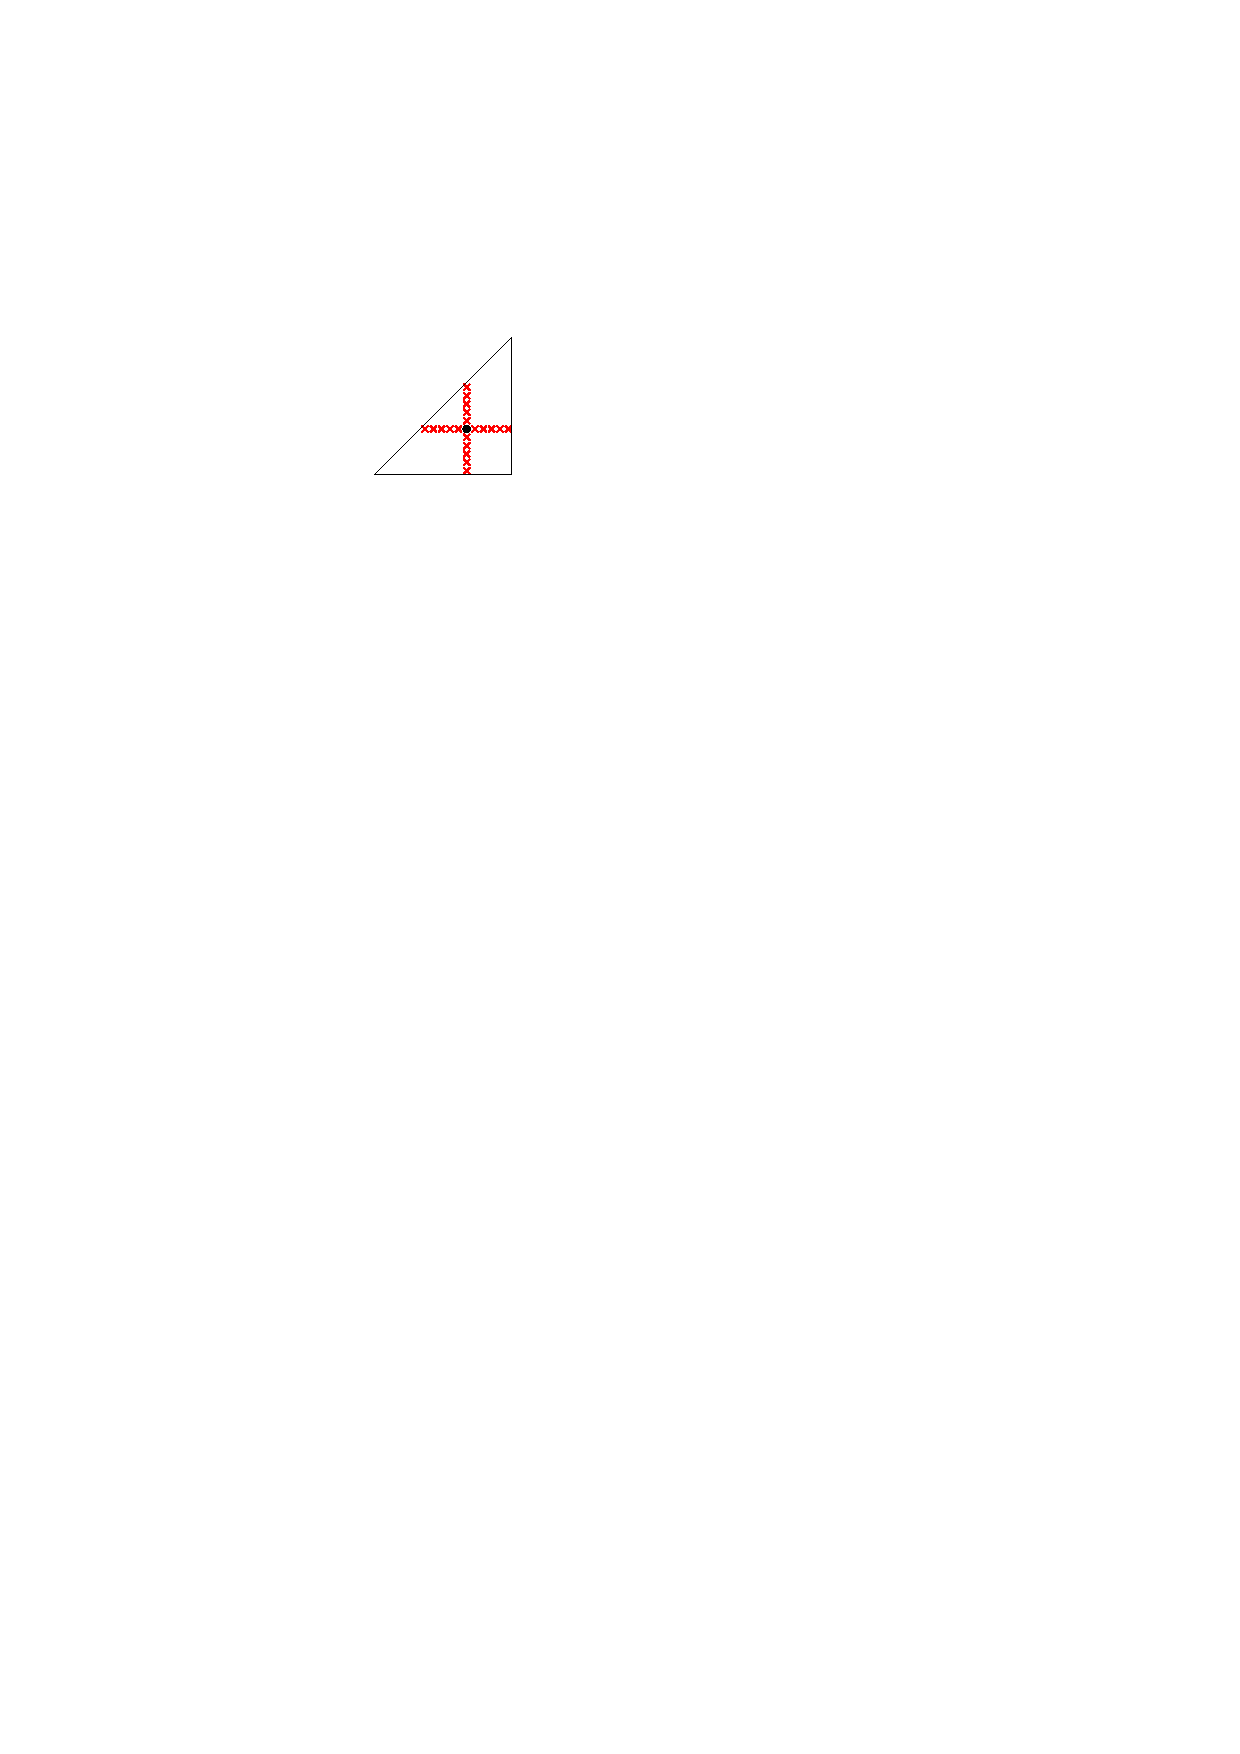
\includegraphics[scale=.8]{figs/killersb-2} \break% 
%           $\{(x,y')\} \cup \{(x',y)\}$ \\
%$\bat$ & 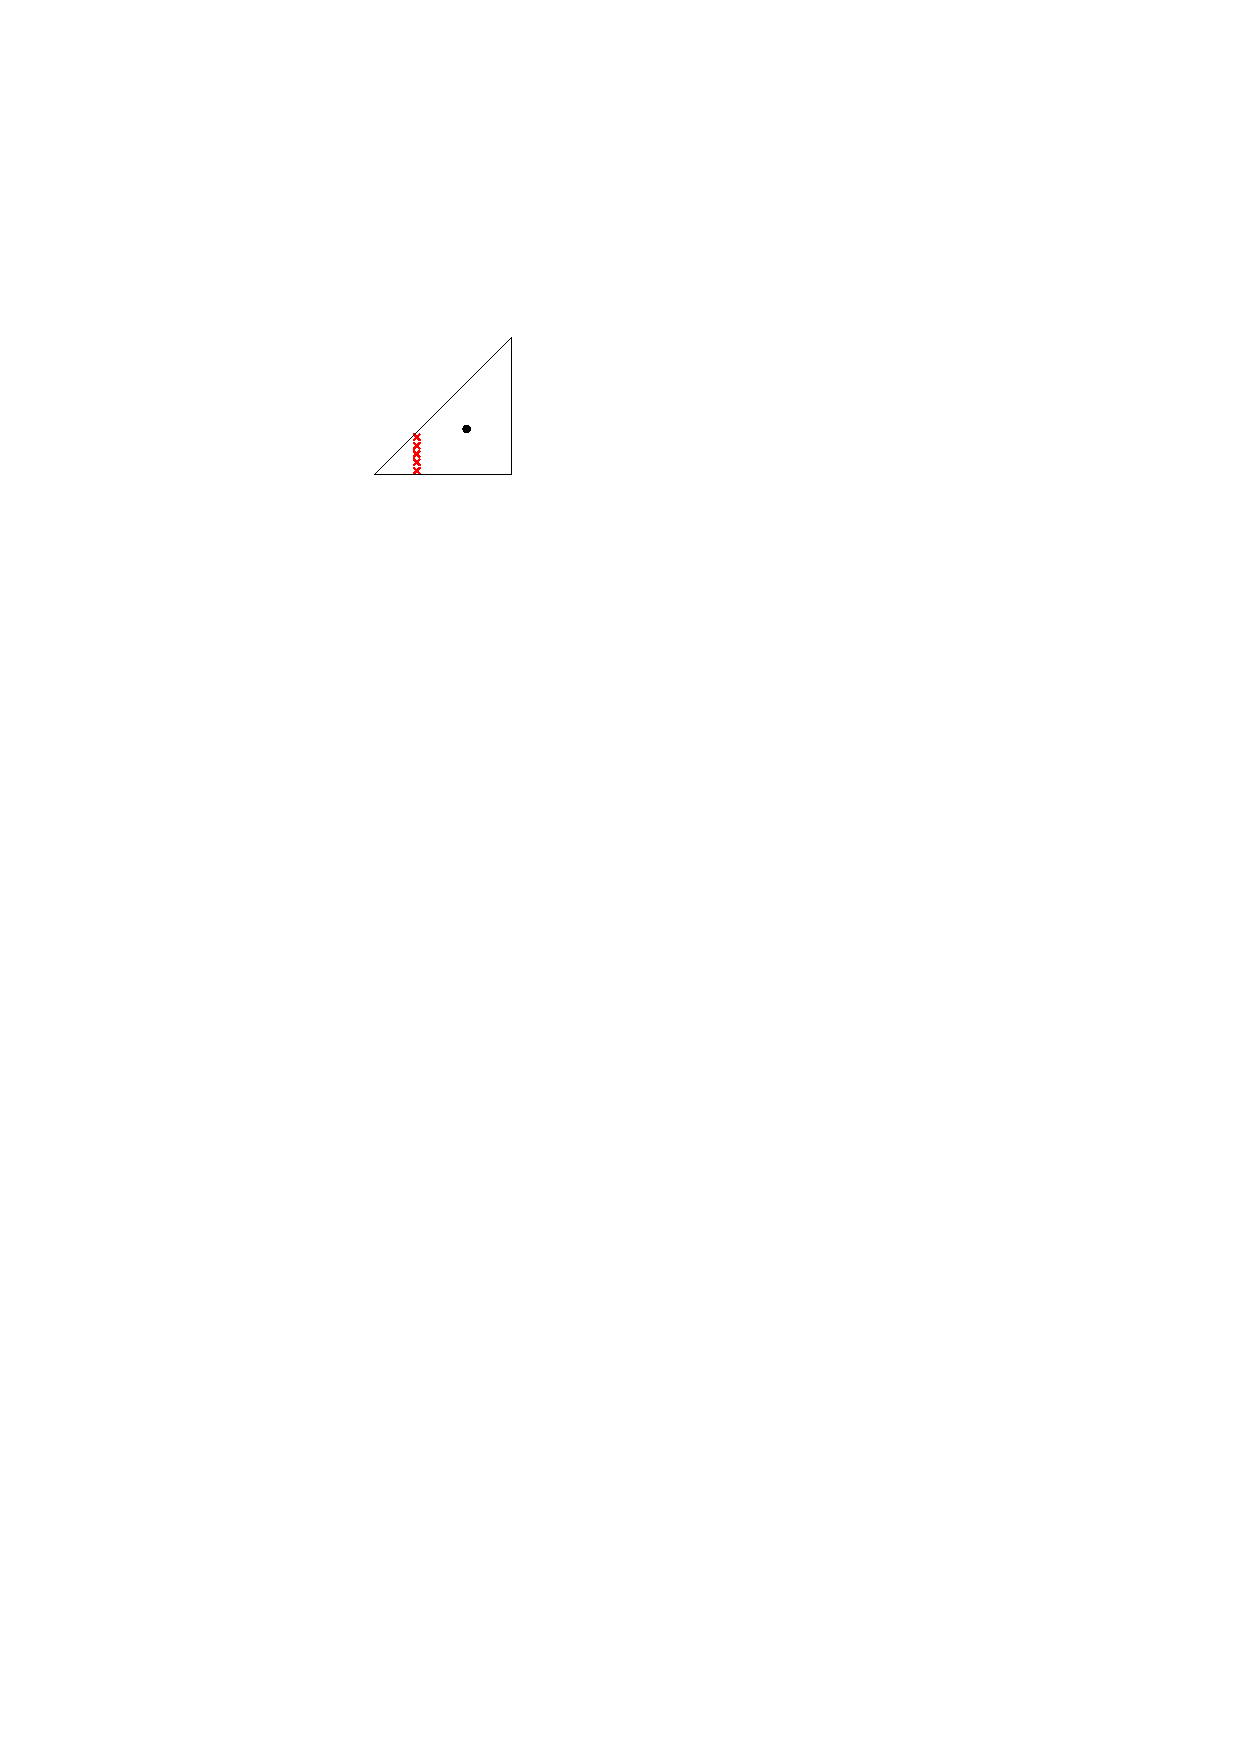
\includegraphics[scale=.8]{figs/killers-3} \break% 
%             $\{(x',y) : x'<x \}\cup\{(x,y') : y'<y \}$ 
%           & 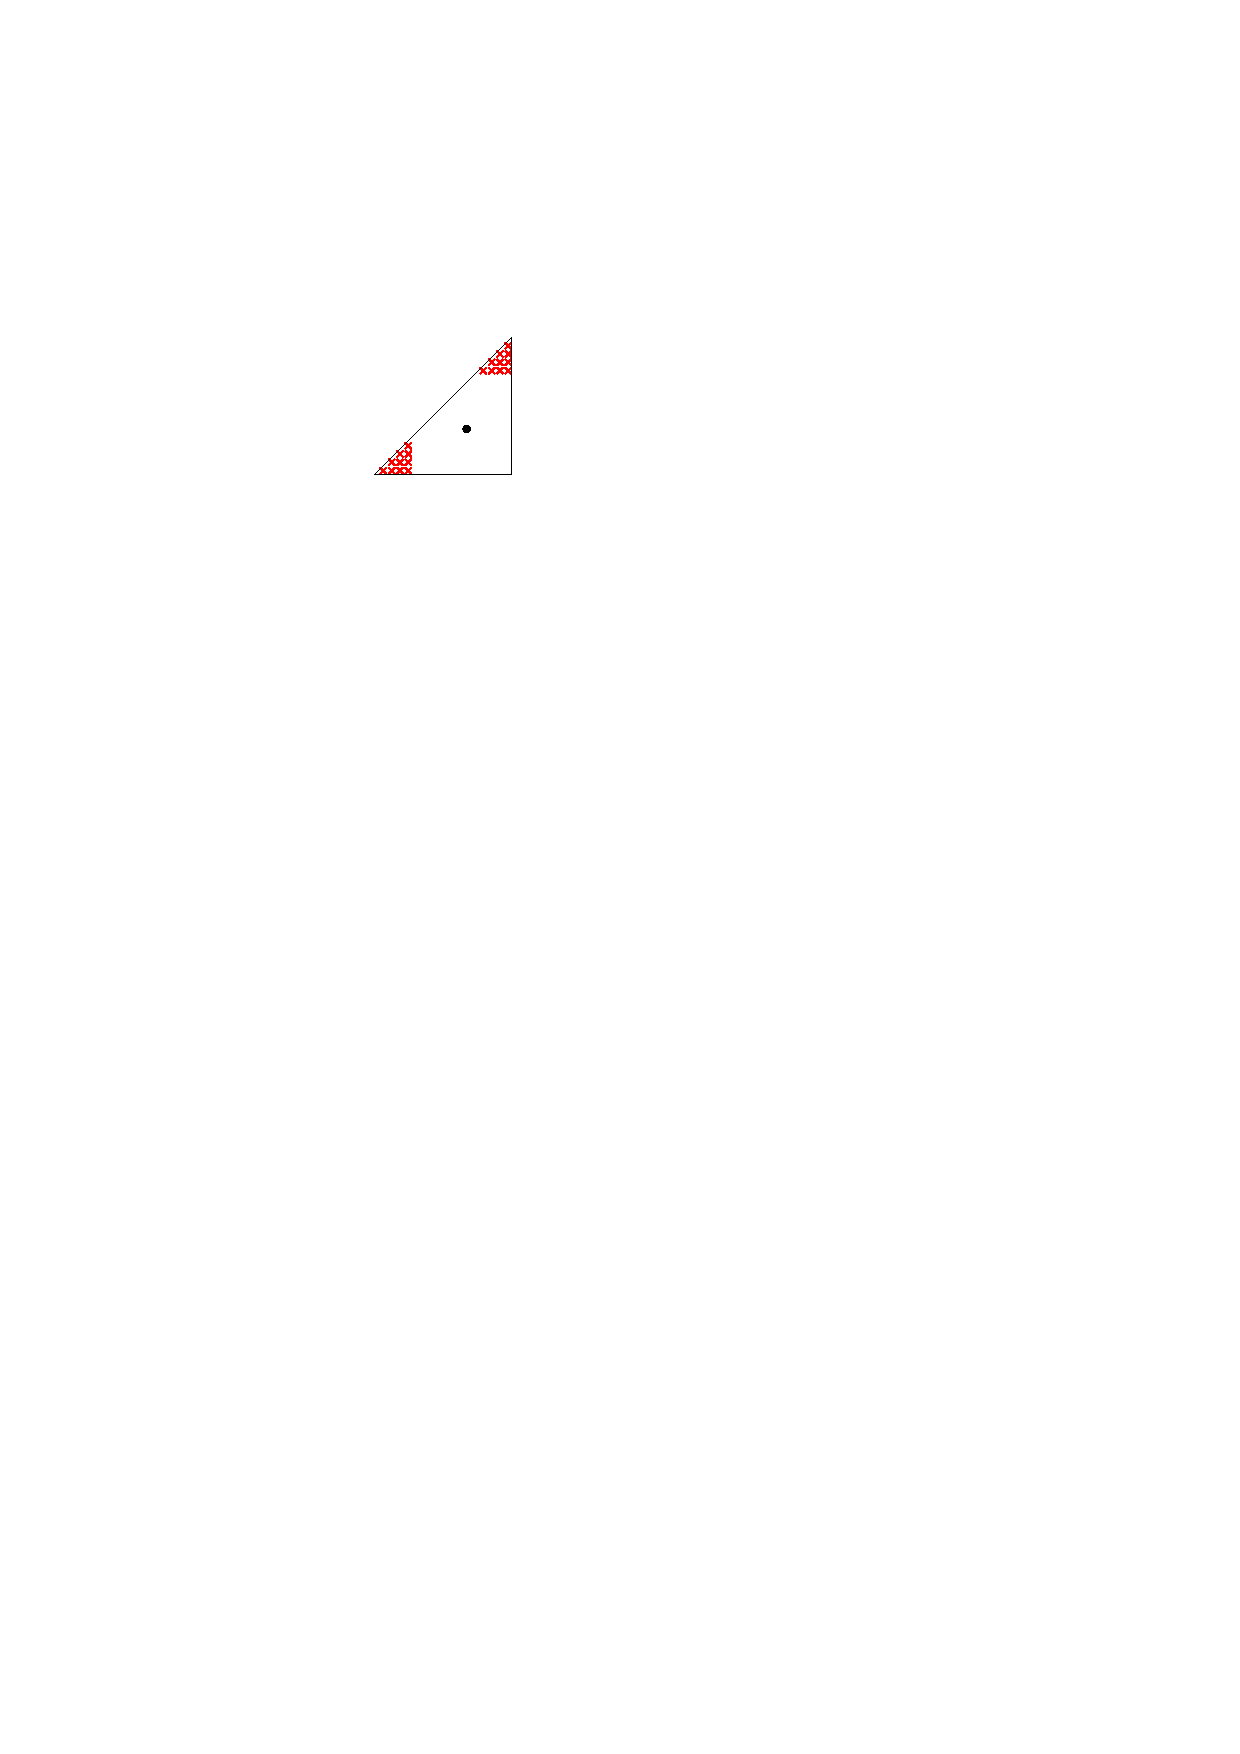
\includegraphics[scale=.8]{figs/killersb-3} \break%
%             $\{(x',y'): x' < y\text{ or } y'> x\}$ \\
%$\nested$ &  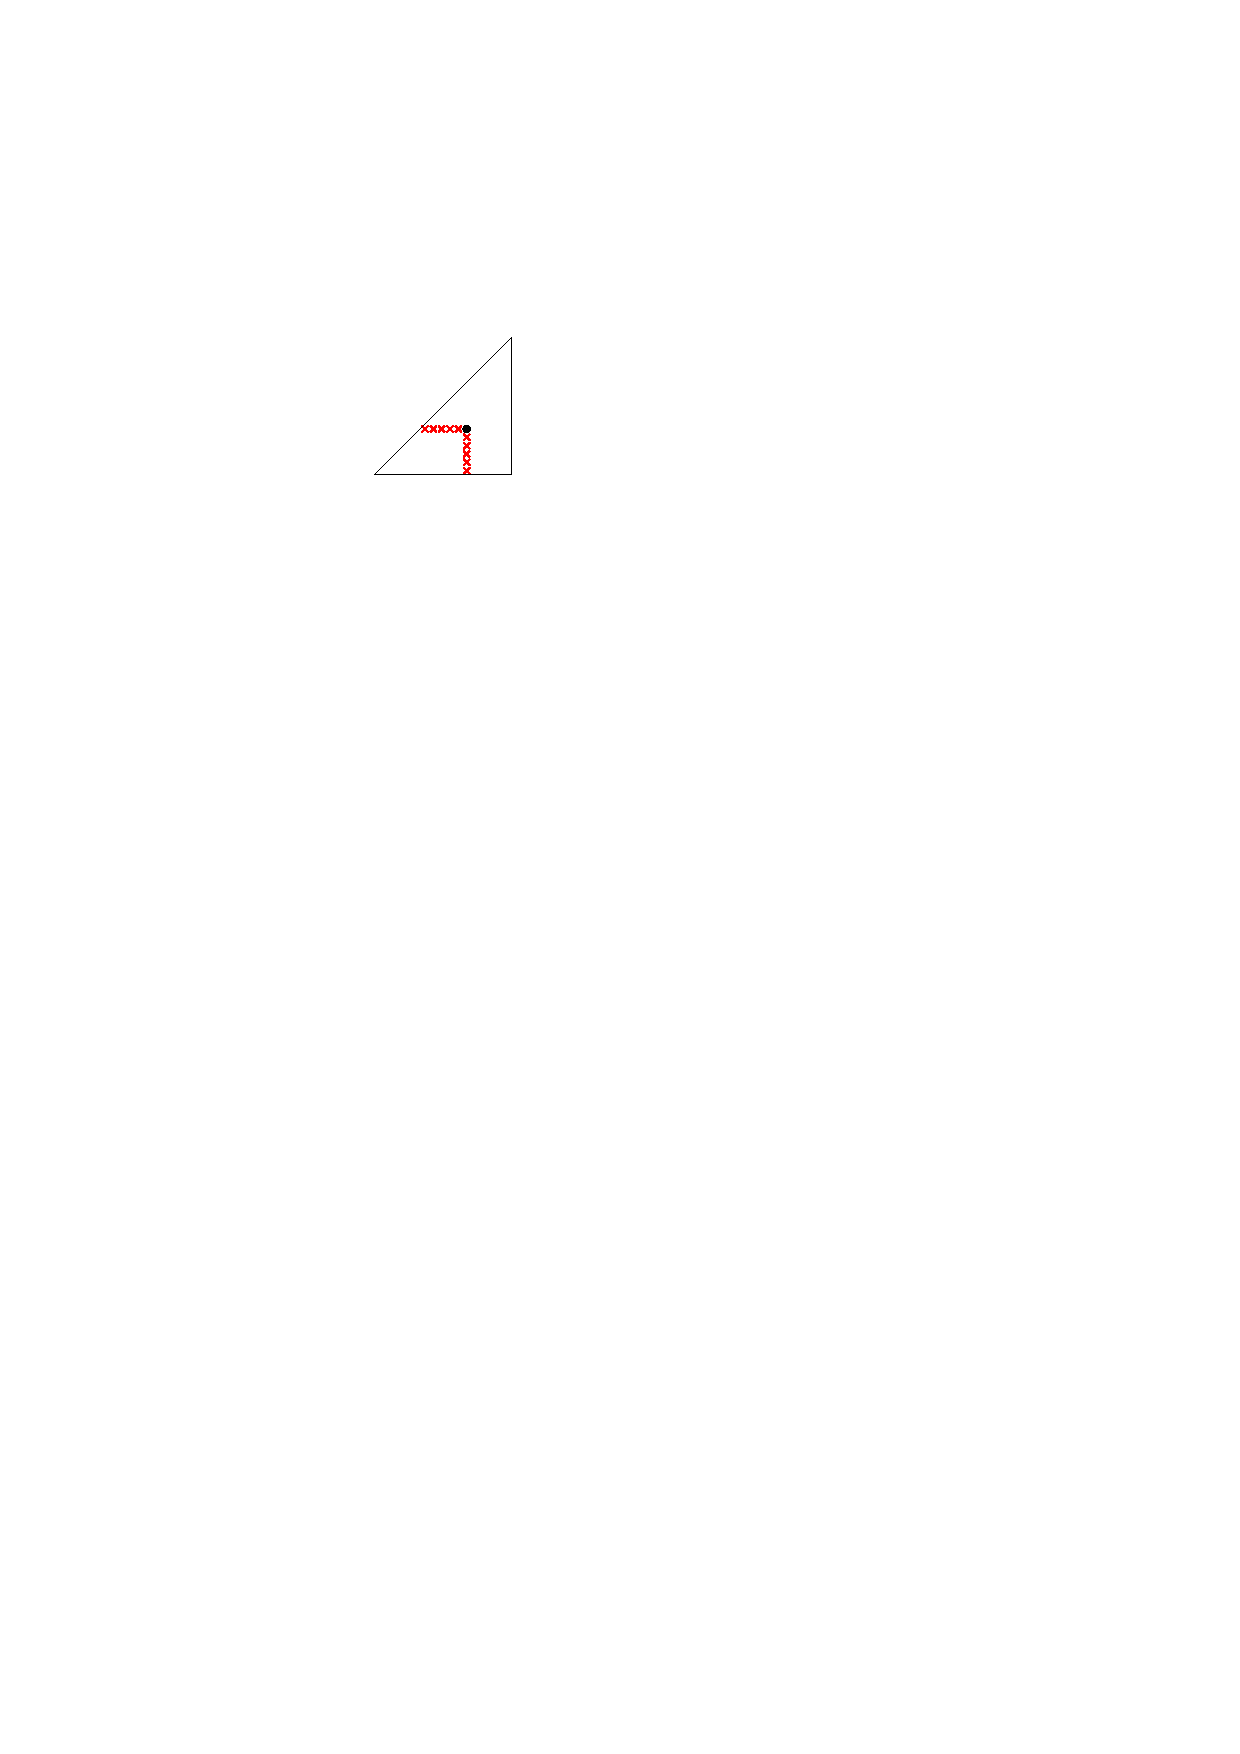
\includegraphics[scale=.8]{figs/killers-4} \break%
%              $\{(x',y) : x'<x \}\cup\{(x,y') : y'<y \}$ 
%         &  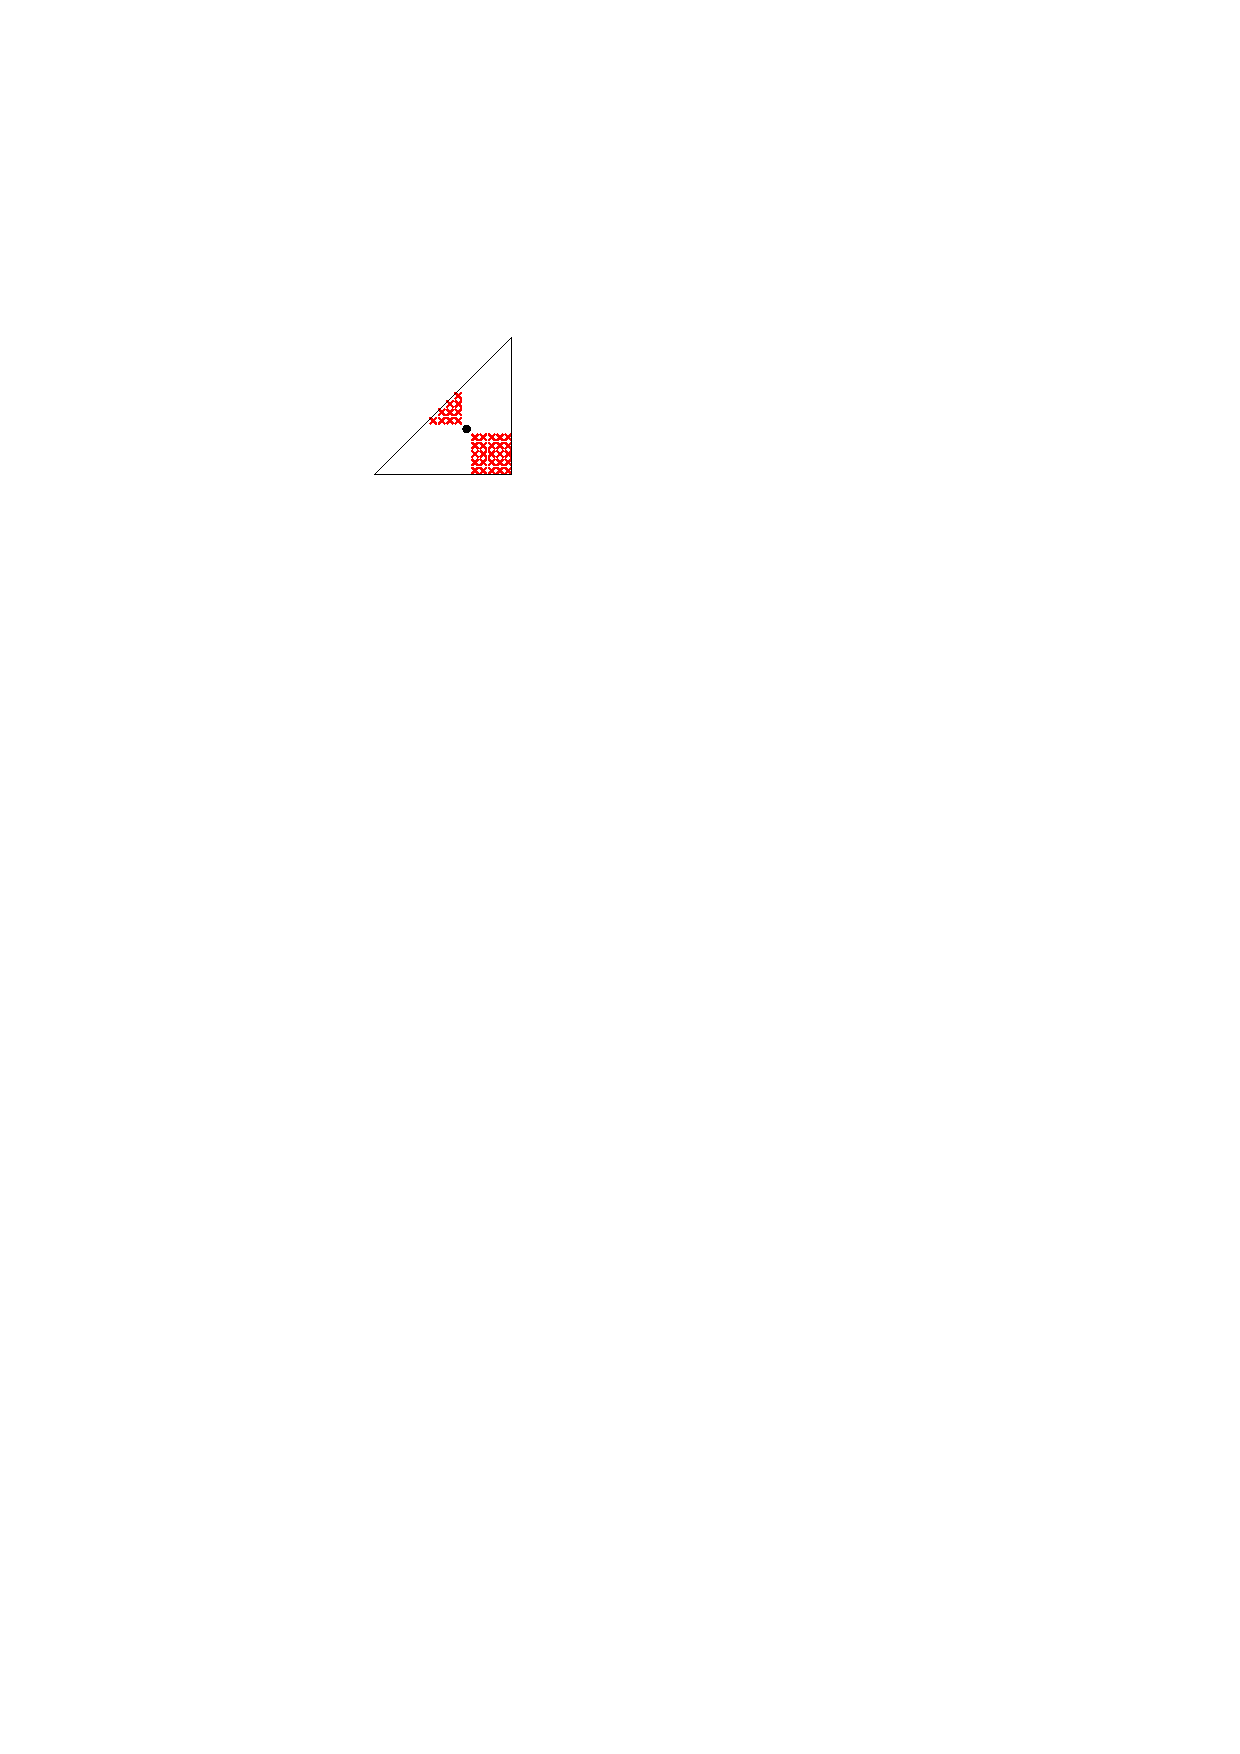
\includegraphics[scale=.8]{figs/killersb-4} \break%
%            $\{(x',y'):\sign(x'-x)=\sign(y-y')\}$ \\
%$\crossing$ &  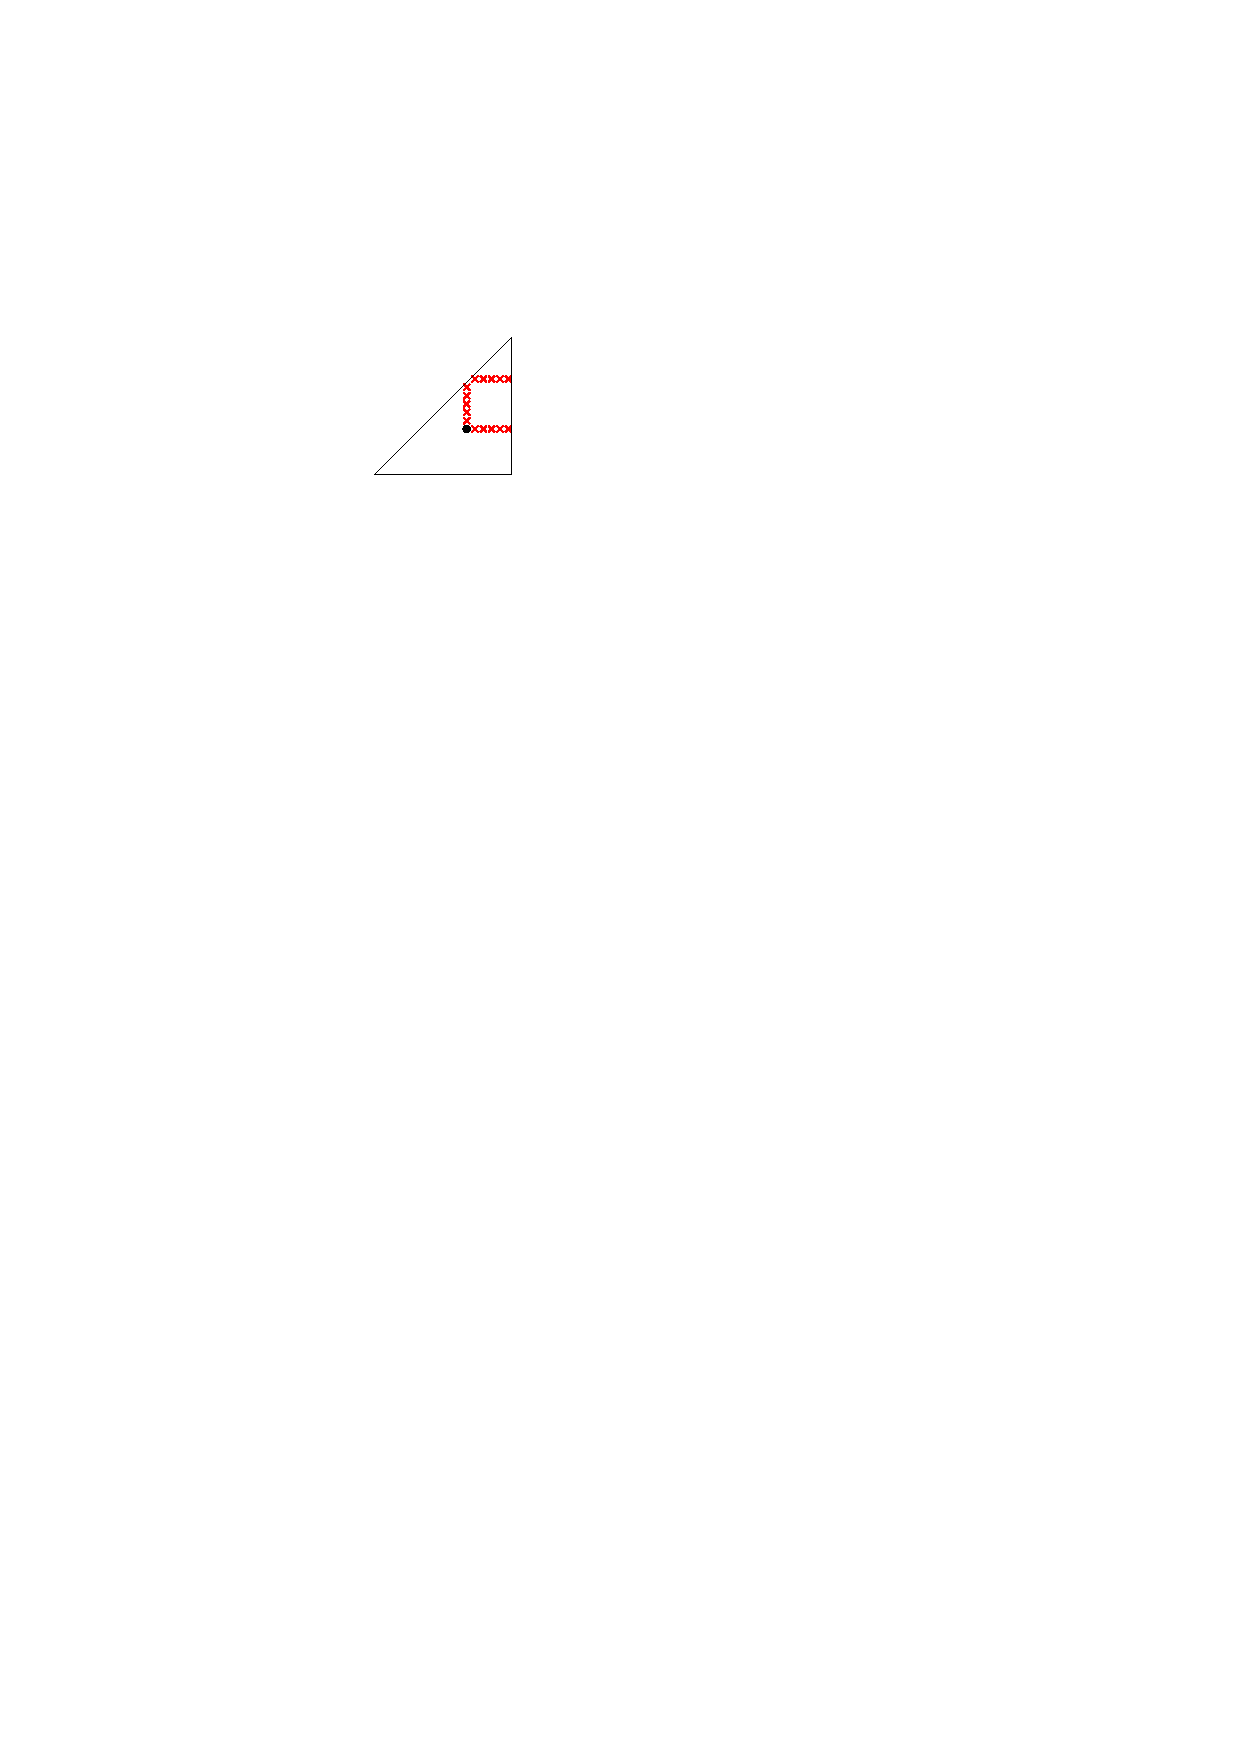
\includegraphics[scale=.8]{figs/killers-5} \break% 
%              $\{(x',y) : x'>x \}\cup\{(x,y') : y'>y \}$ 
%         &  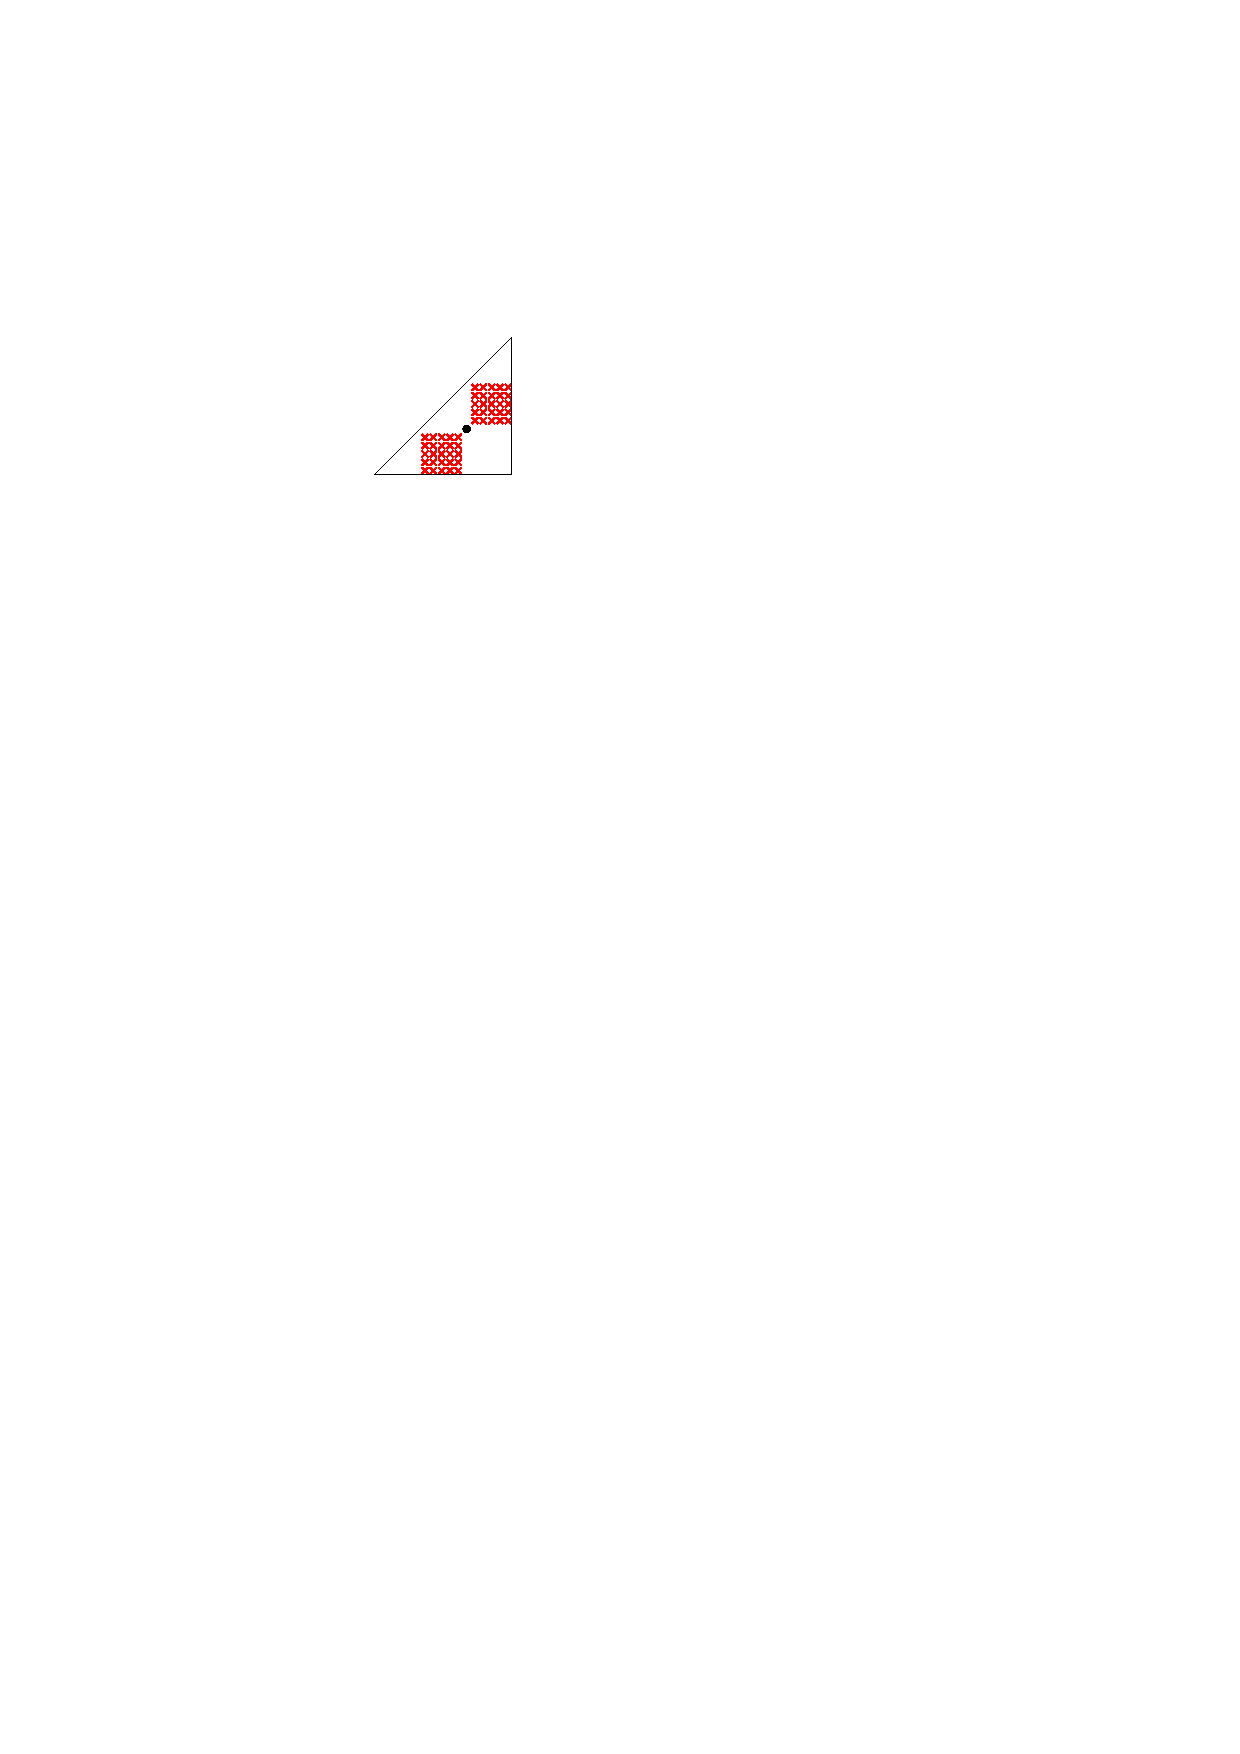
\includegraphics[scale=.8]{figs/killersb-5} \break% 
%            $\{(x',y'):\sign(x'-x)=\sign(y'-y)\}$ \\
%$\ears$ &  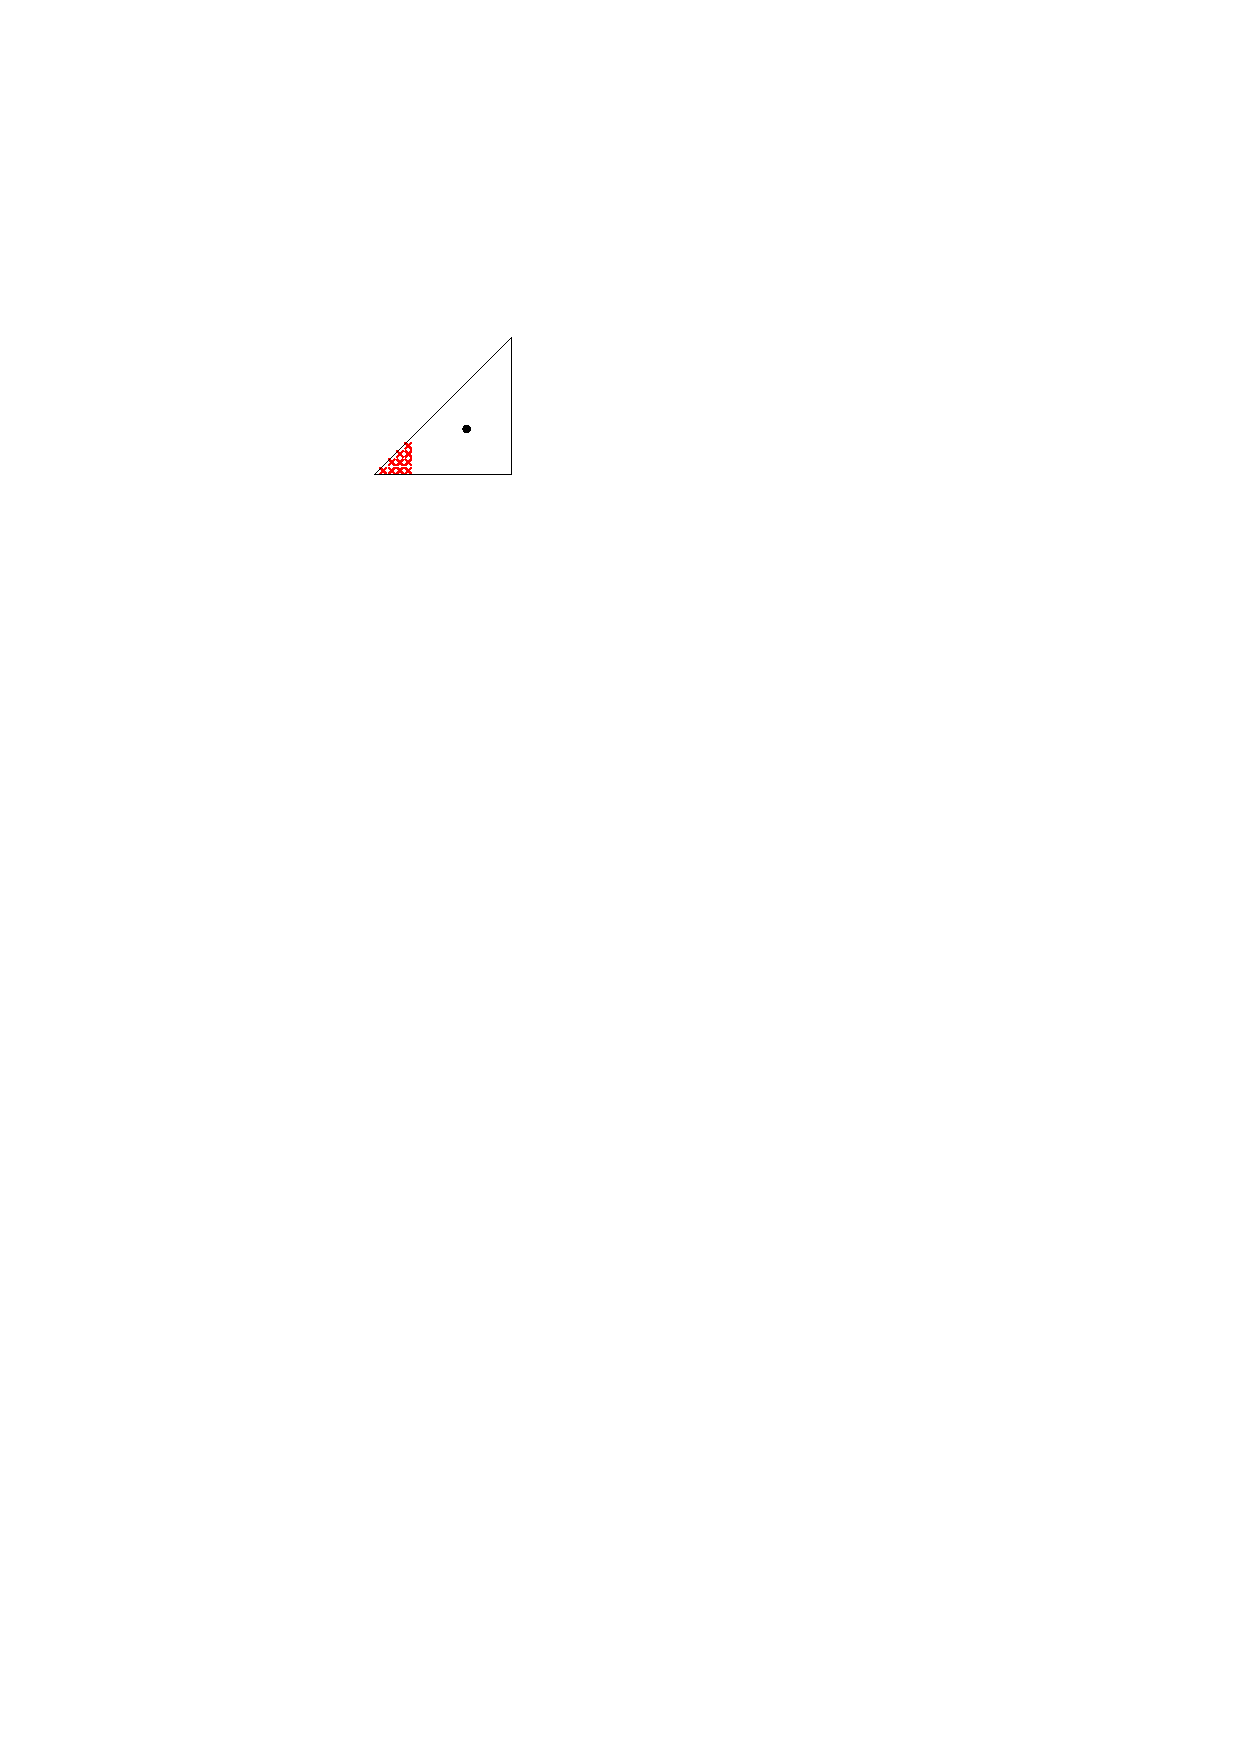
\includegraphics[scale=.8]{figs/killers-6} \break%
%                $\{(x',y'): x'< y\}$
%         & 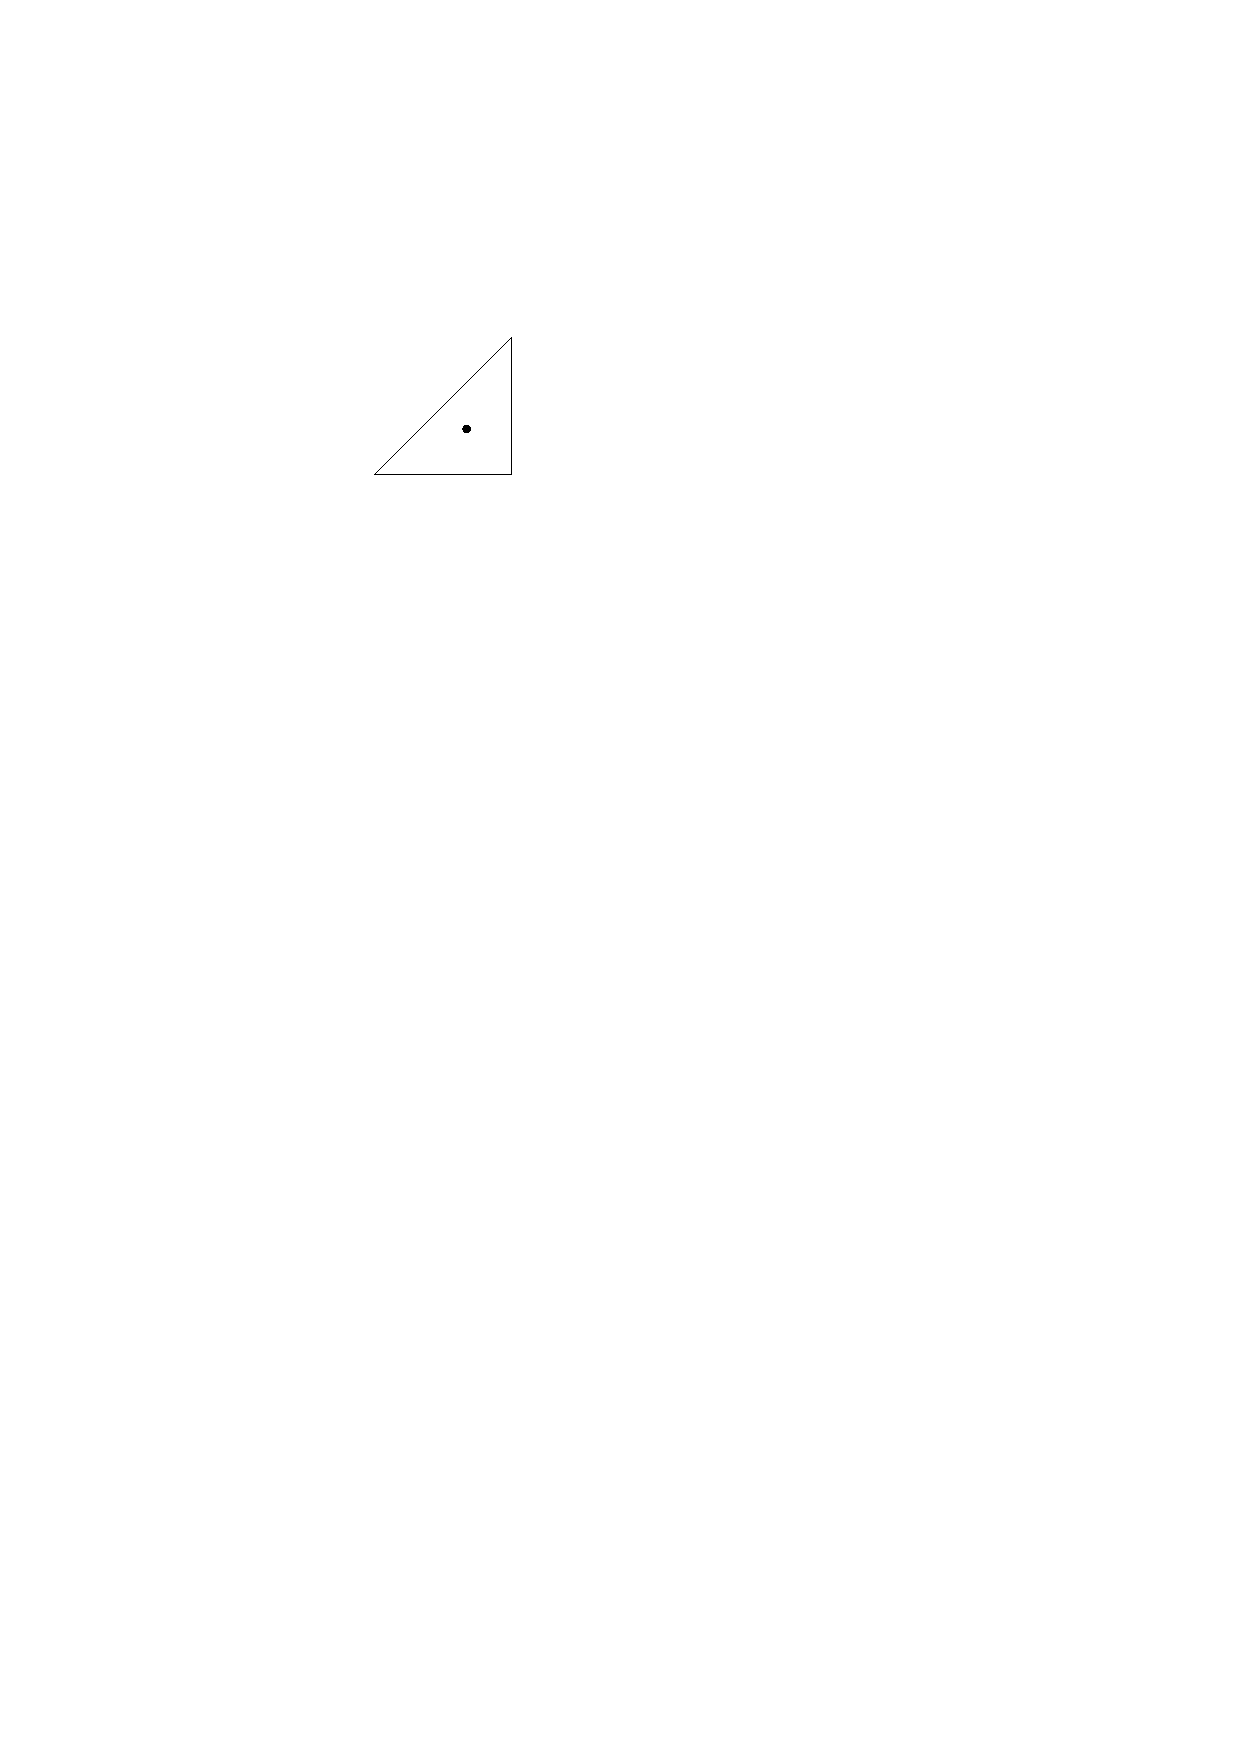
\includegraphics[scale=.8]{figs/killersb-6} \break%
%           $\{\}$ \\
%$\swords$ & 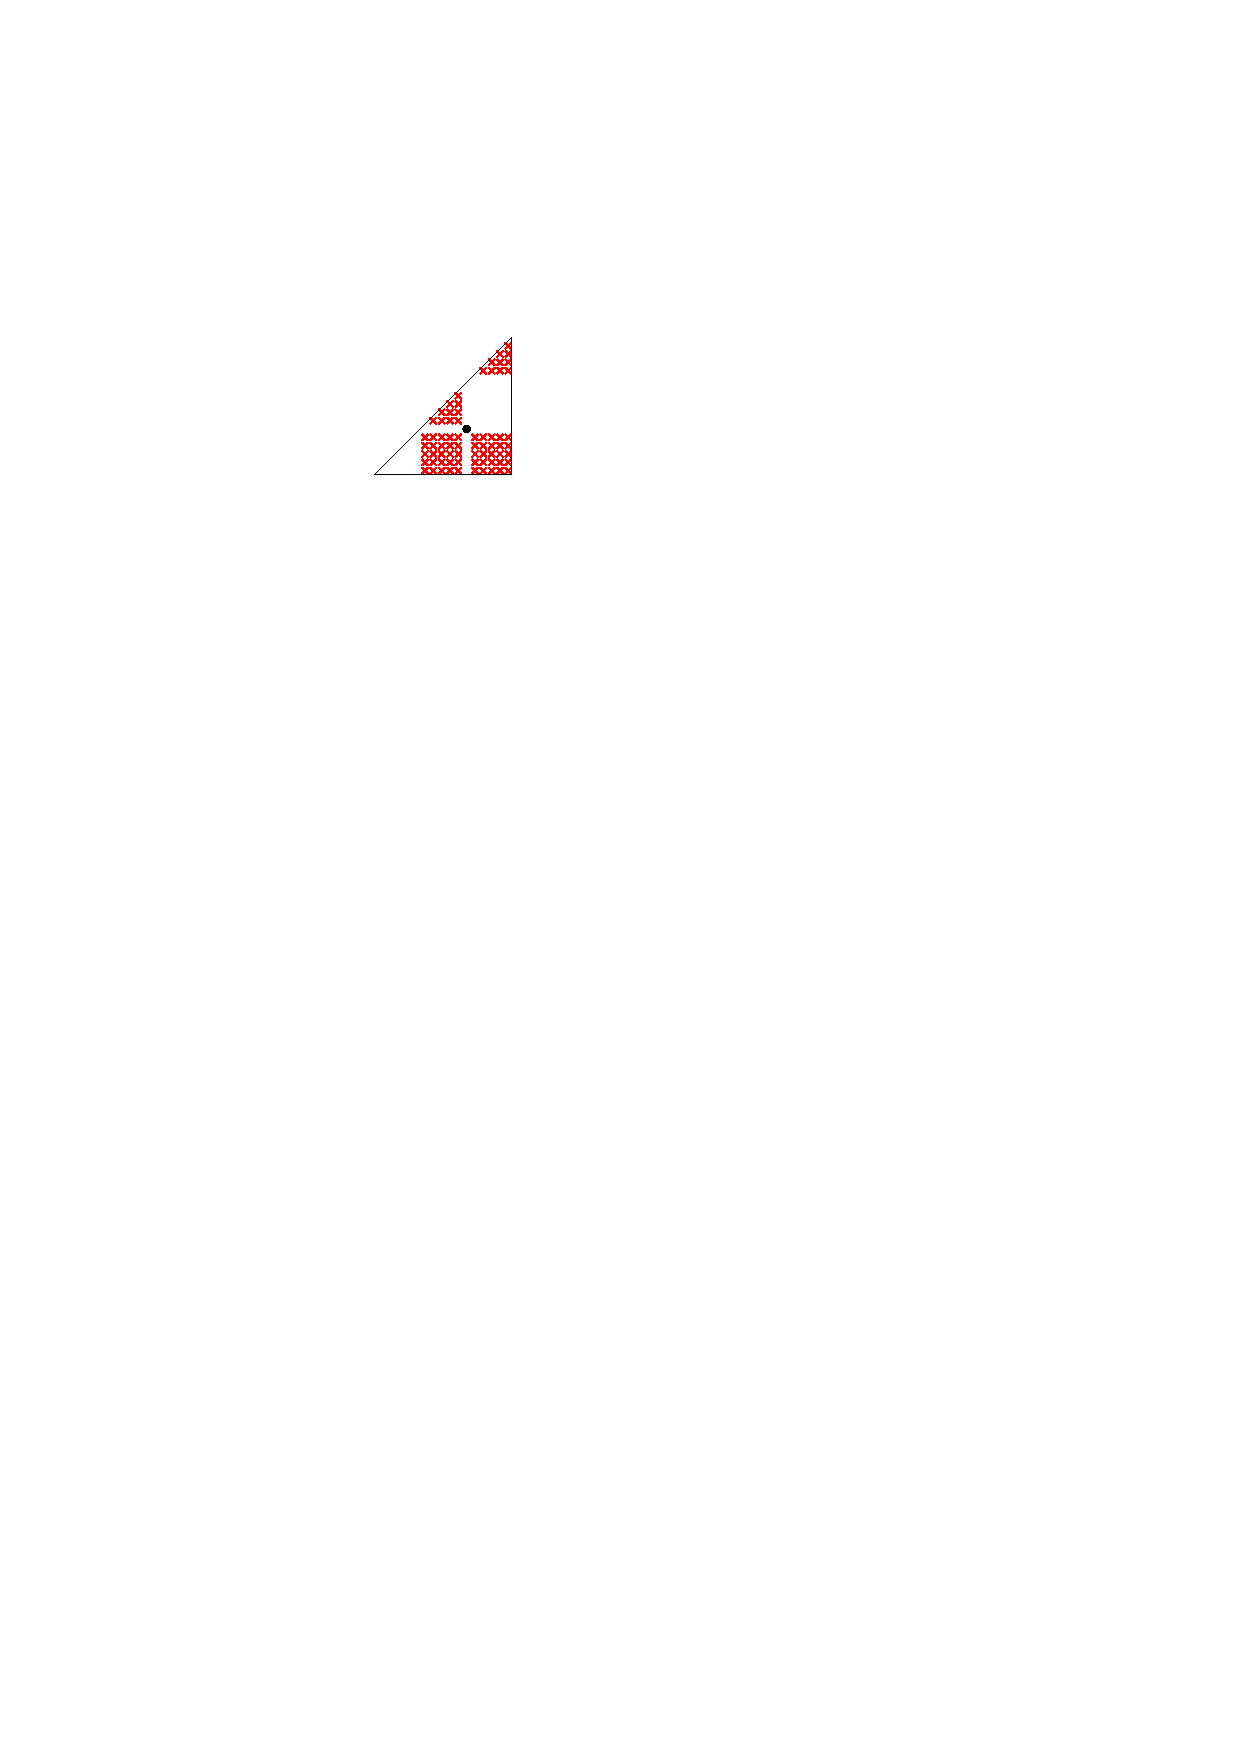
\includegraphics[scale=.8]{figs/killers-7} \break%
%               $\{(x',y'): x'>x, y'< y\}$
%         & 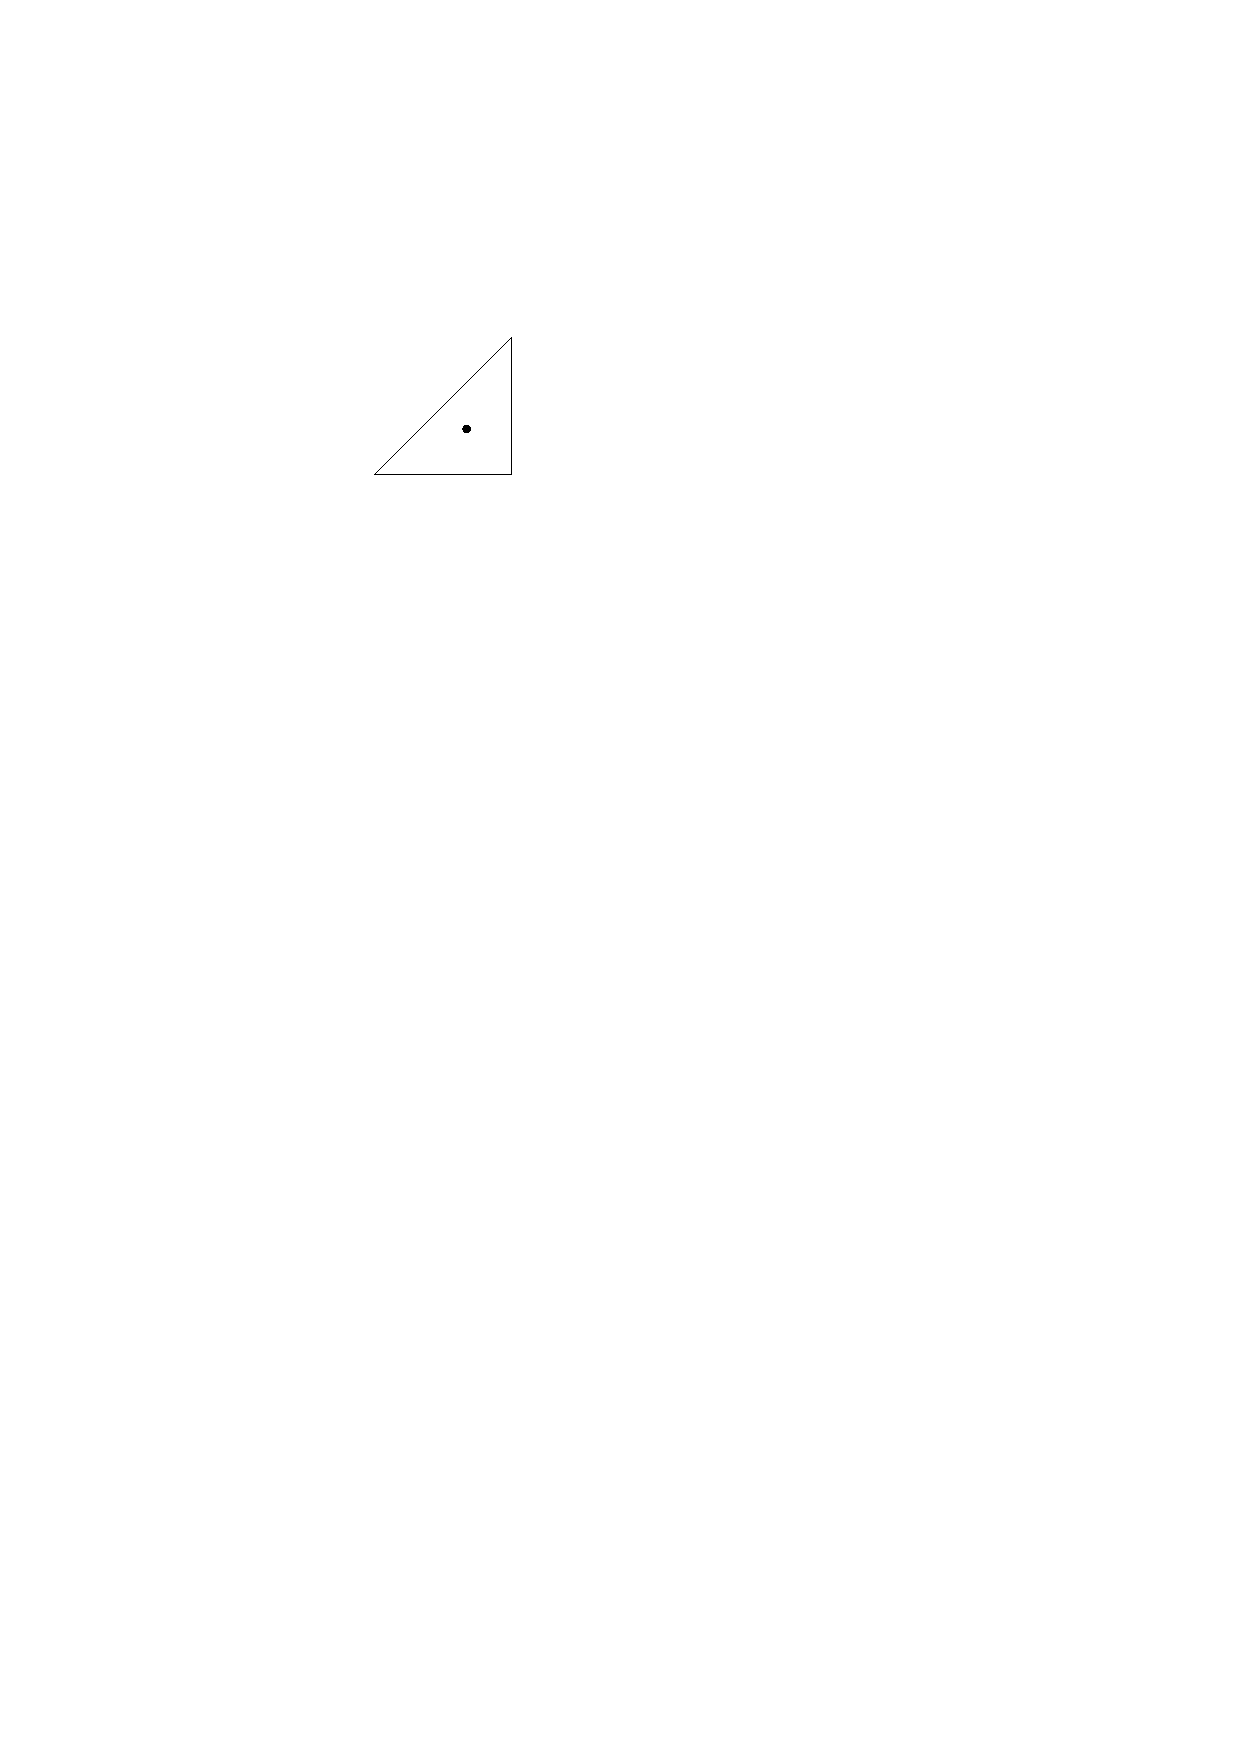
\includegraphics[scale=.8]{figs/killersb-7} \break%
%           $\{\}$ \\
%$\david$ &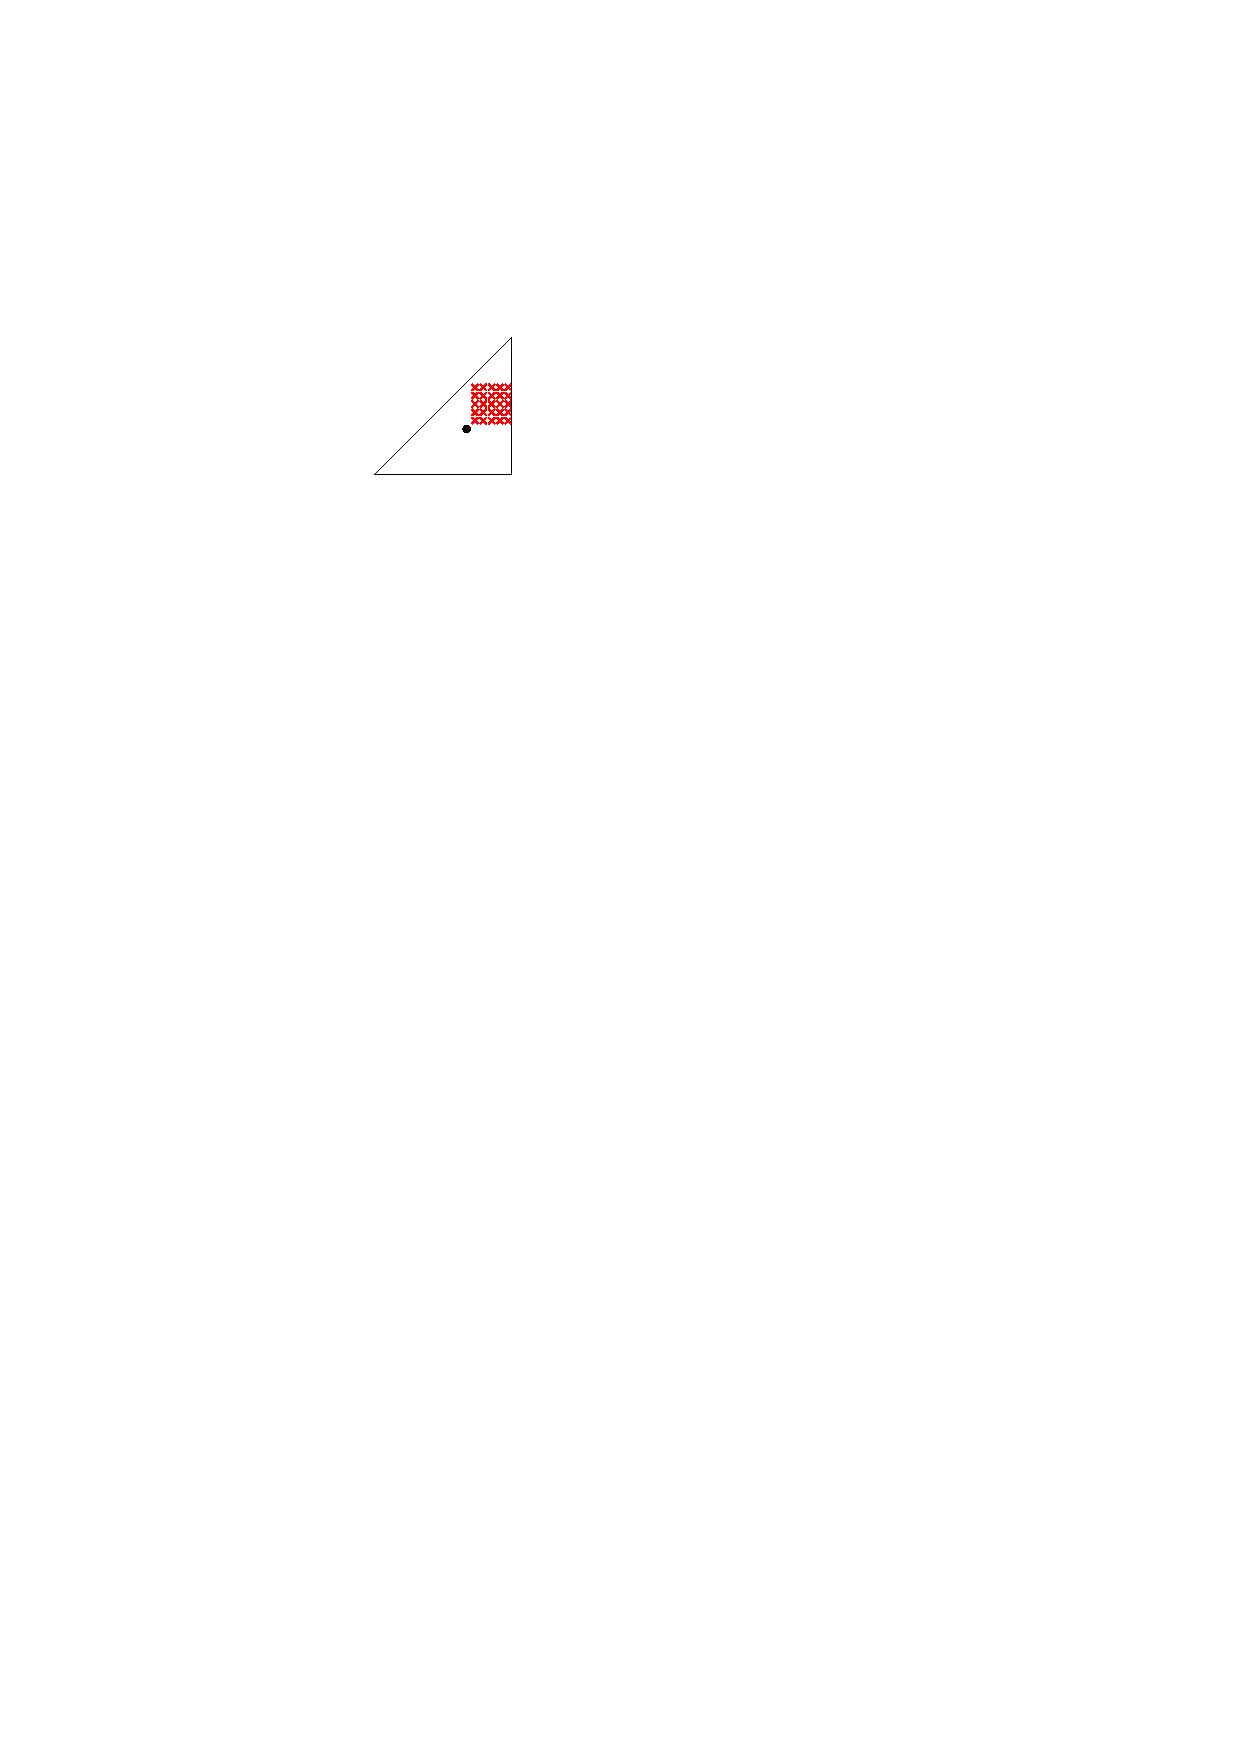
\includegraphics[scale=.8]{figs/killers-8} \break%
%               $\{(x',y'): y < y' <x,\,\, x'>x\}$
%         & 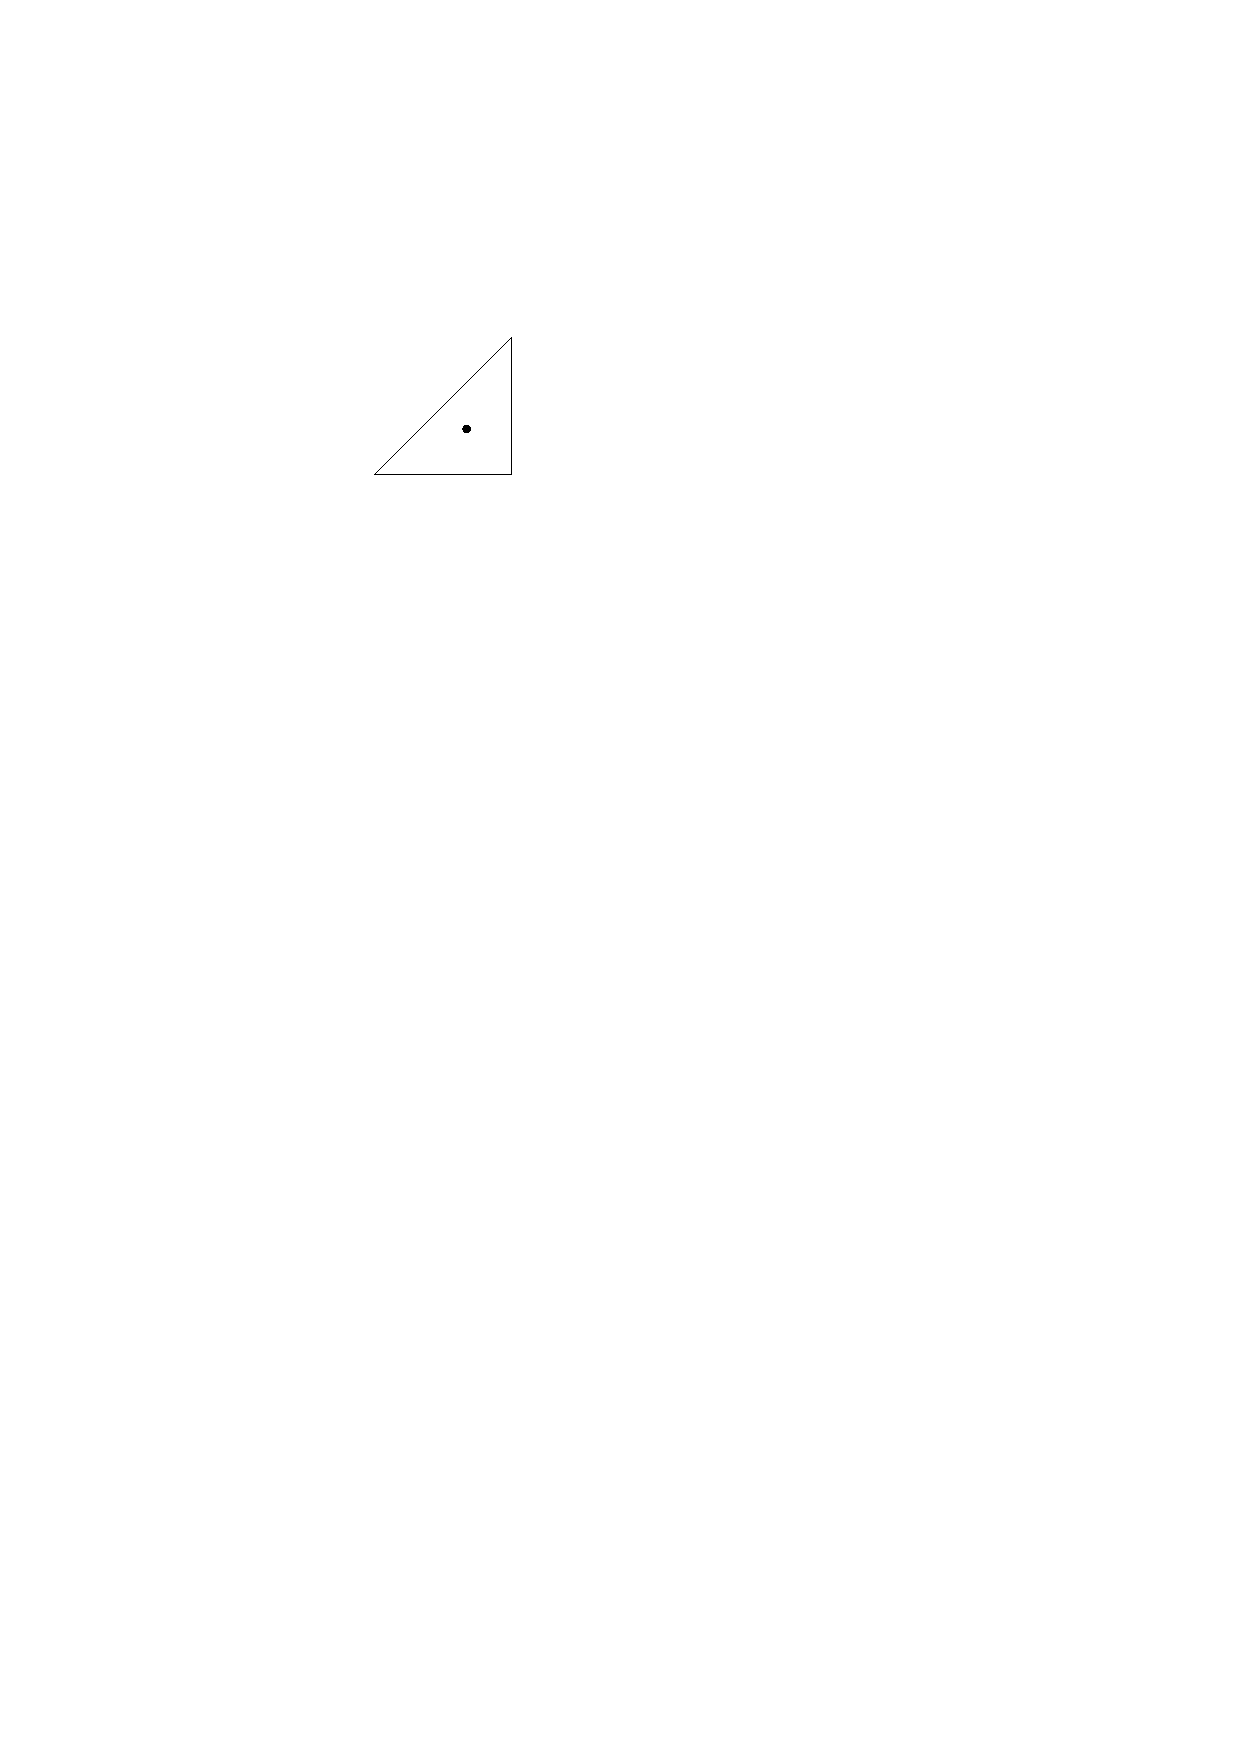
\includegraphics[scale=.8]{figs/killersb-8} \break%
%           $\{\}$ \\
%\end{tabular}
%\end{center}
%   \caption{The restrictions placed on the dot puzzle when for each of 
%     the forbidden subconfigurations.}
%   \tablabel{forbidden}
%\end{table}
%

\begin{figure}
   \begin{center}
      \newlength{\ka}
      \setlength{\ka}{\textwidth}
      \addtolength{\ka}{-1cm}
      \begin{tabular}{c@{\hspace{1cm}}c}
        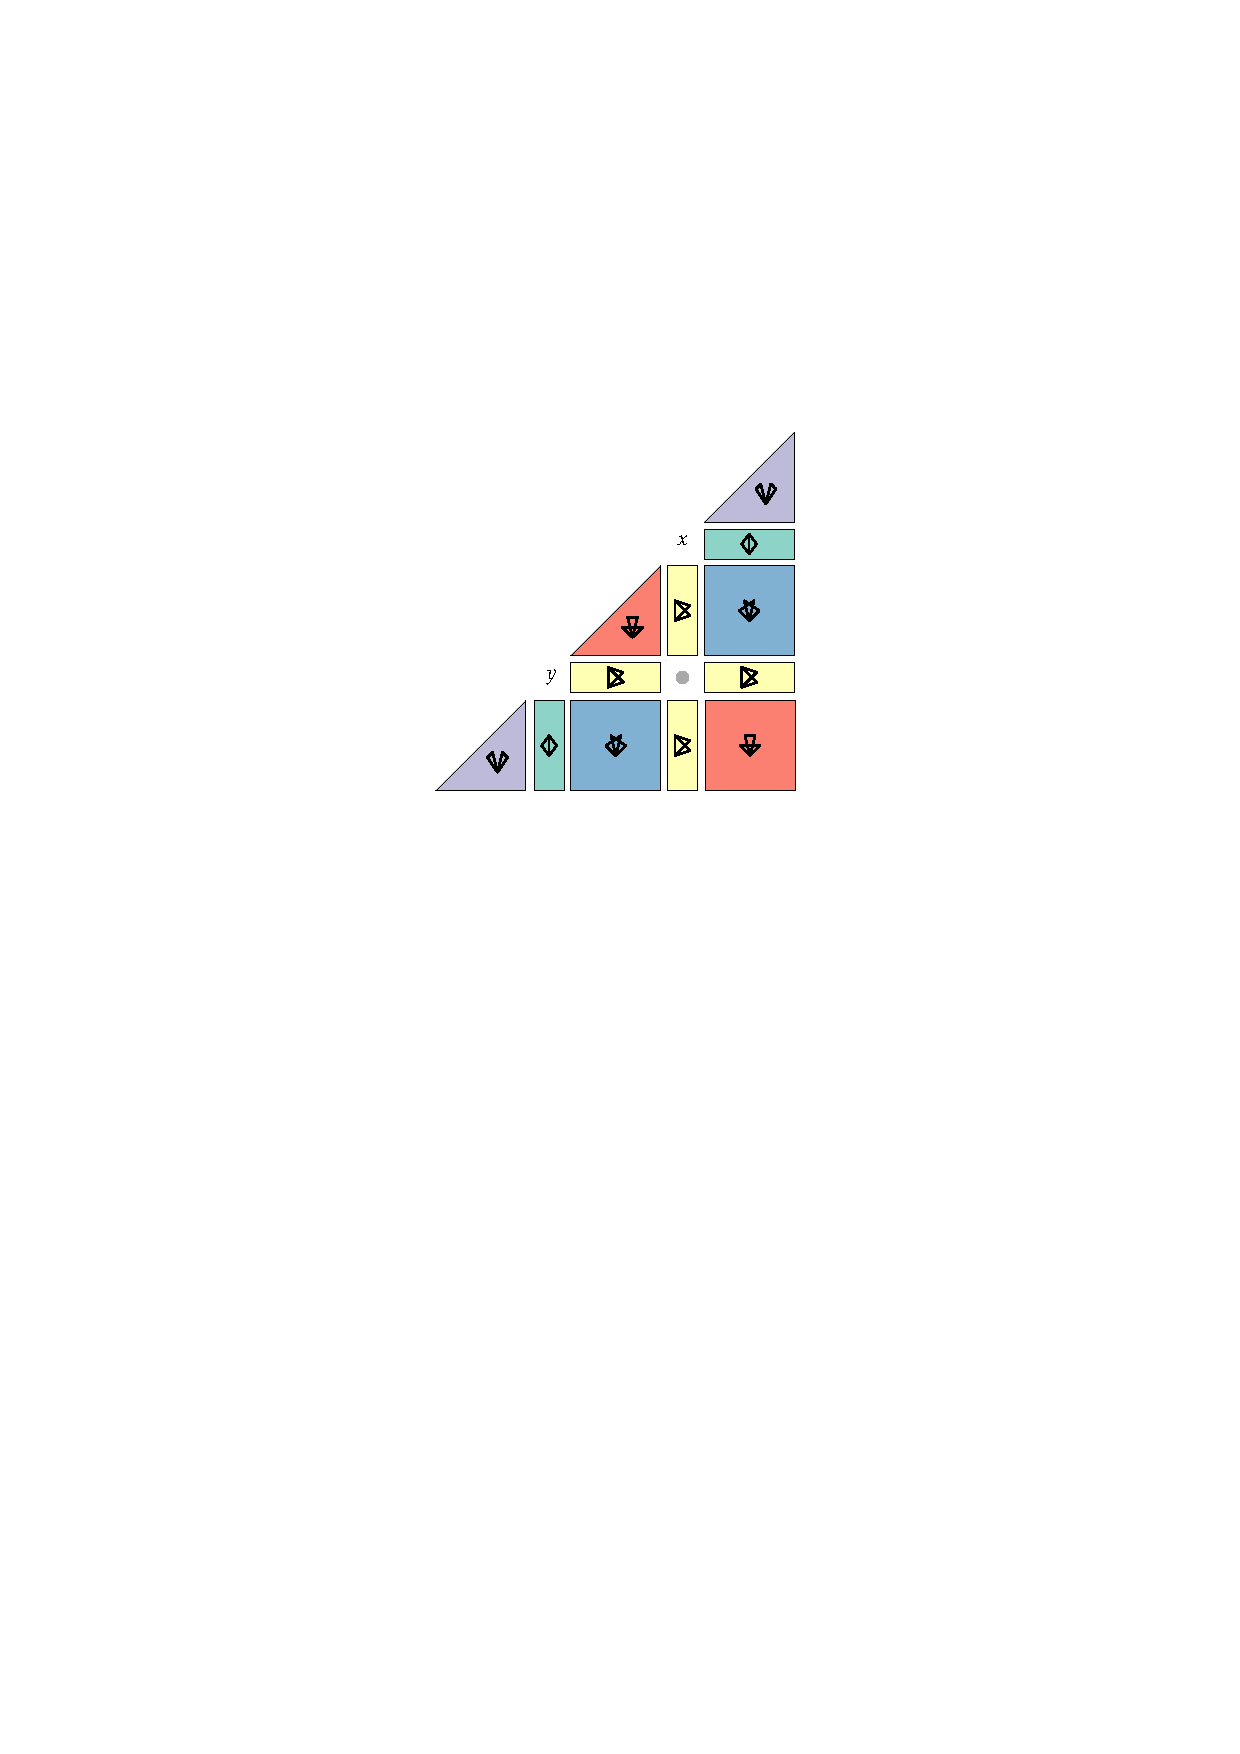
\includegraphics[width=.48\ka]{figs/crapper-2} & 
        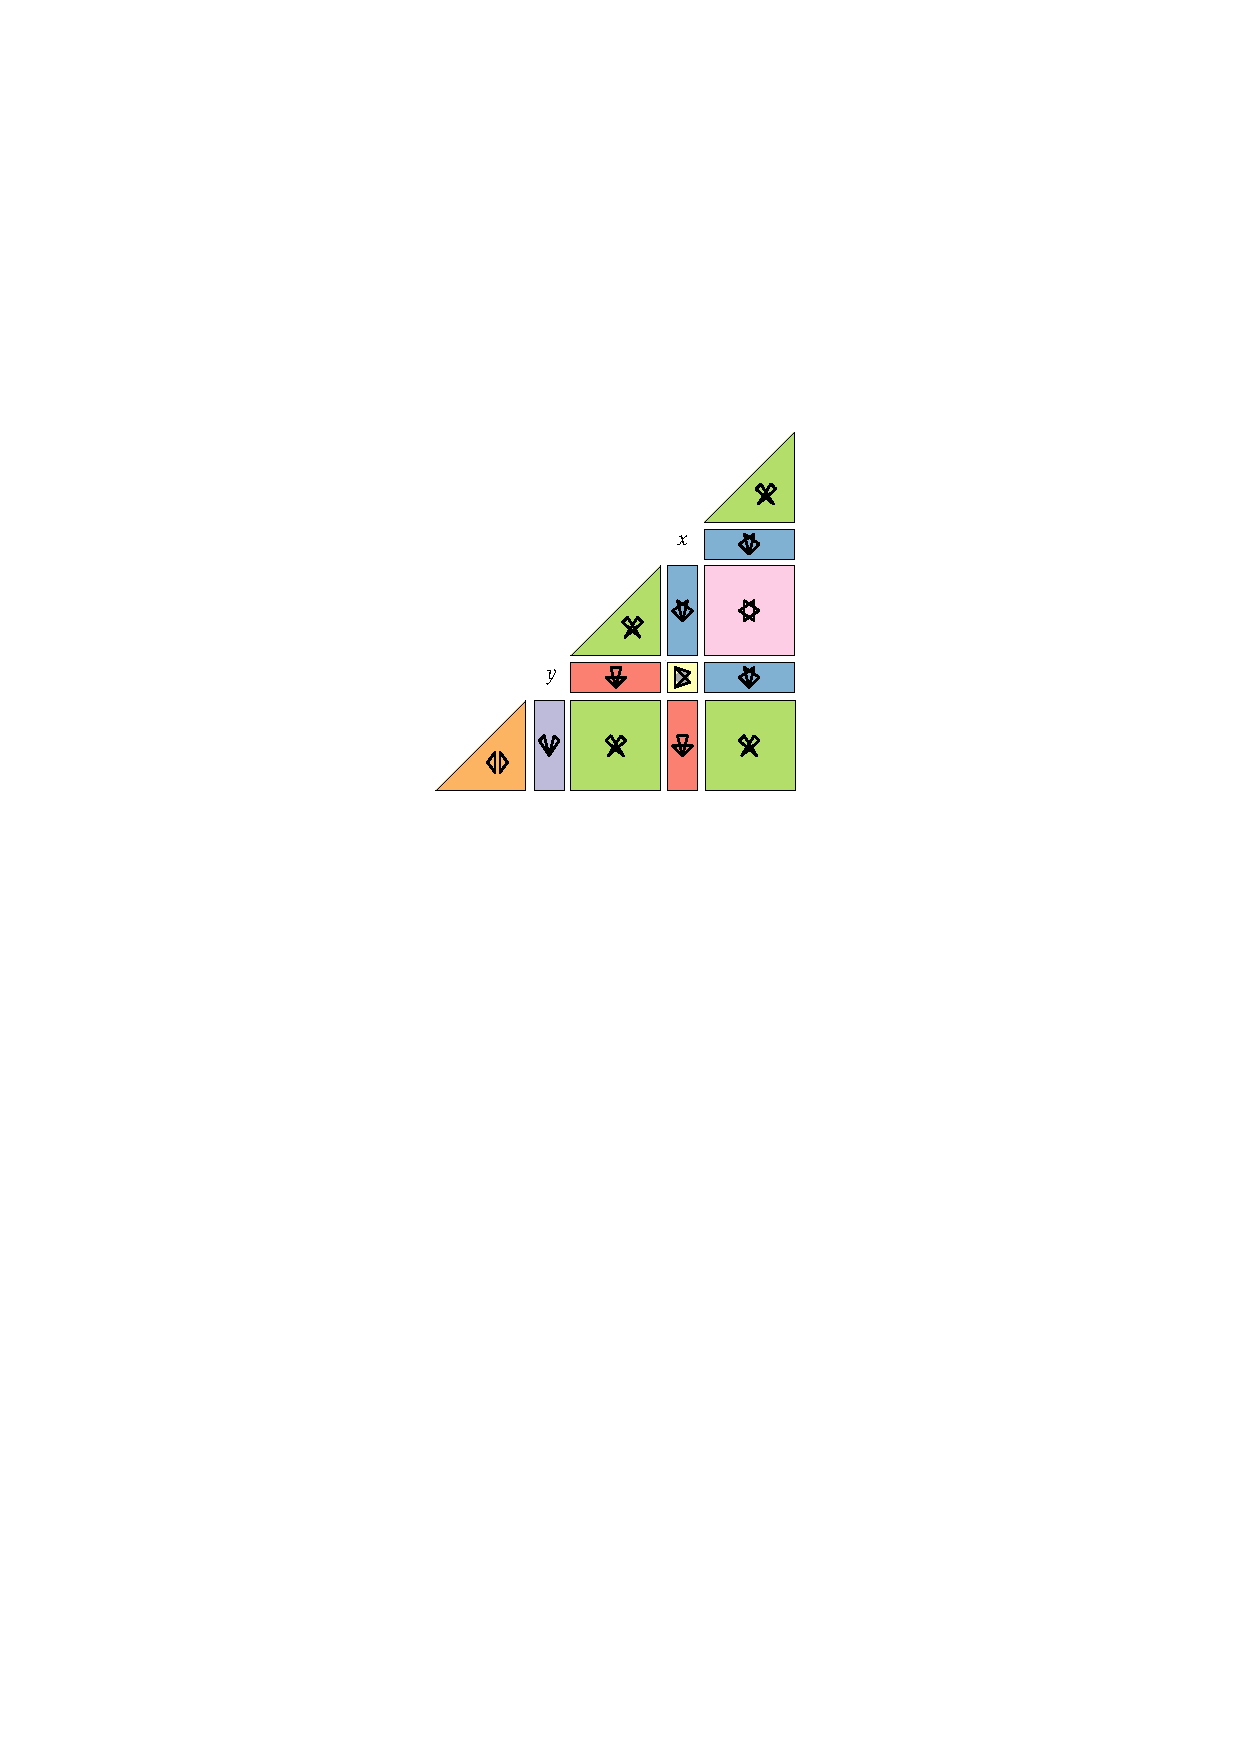
\includegraphics[width=.48\ka]{figs/crapper-1} \\
        (a) & (b)
      \end{tabular}
   \end{center}
   \caption{The regions killed by forbidden configurations during (a)~the current round and (b)~subsequent rounds.}
   \figlabel{forbidden-color}
\end{figure}


\subsection{Some Easy Bounds}

We say that a point set is \emph{non-decreasing} (respectively,
increasing, non-increasing, decreasing) if, when sorted lexicographically,
the $y$ coordinates of the points form a non-decreasing (respectively,
increasing, non-increasing, decreasing) sequence.

From \figref{forbidden-color}, some previous upper bounds naturally
fall out.  For example, Bra\ss's results \cite{brass:turan} that
$\ex(\nested)\in O(n^2)$ comes from the fact points selected during a
single round of the dot puzzle must be non-decreasing, and thus at most
$2n-3$ points can be selected take part in $Q_i$ during a round $i$.
Thus $\sum_{j=1}^{n}|Q_i| \le 2n^2-3n$, and the bound $\ex(\nested)\in
O(n^2)$ immediately follow from \lemref{top-bottom}.  Bra\ss's result
that $\ex(n,\crossing)\in O(n^2)$ is obtained in a similar way, using
the fact that the points in any $Q_i$ must be non-increasing.

Similarly, we can almost recover the result of Bra\ss, Rote and
Swanepoel \cite{brass.rote.ea:triangles} on $\ex(\ears, \swords,
\bat,\nested)$. 
By forbidding $\nested$, we have the rule
\begin{center}
  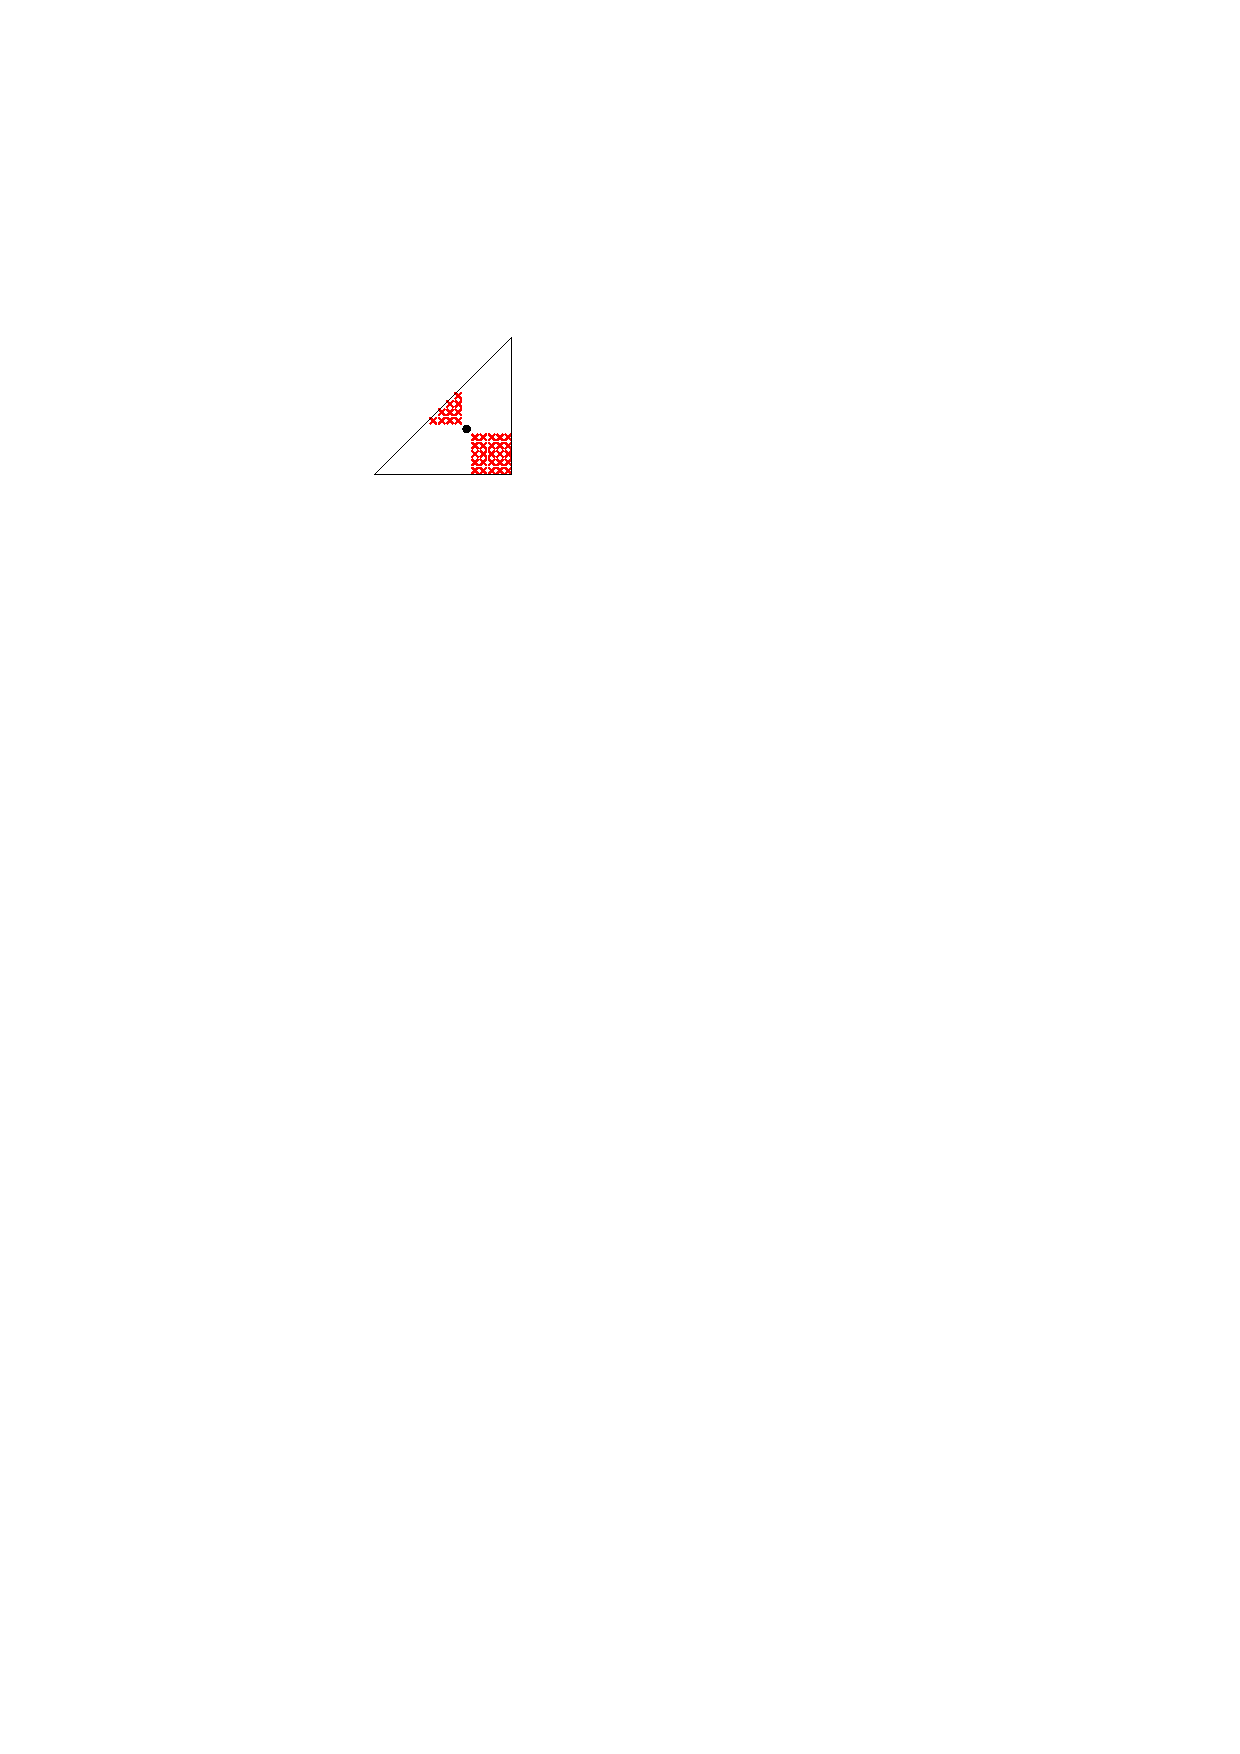
\includegraphics{figs/killersb-4} \enspace ,
\end{center}
which ensures that the set of points taken during a single round form
a non-decreasing point set.  From the forbidden configurations $\bat$,
$\nested$, $\ears$, and $\swords$, we obtain the rule
\begin{center}
  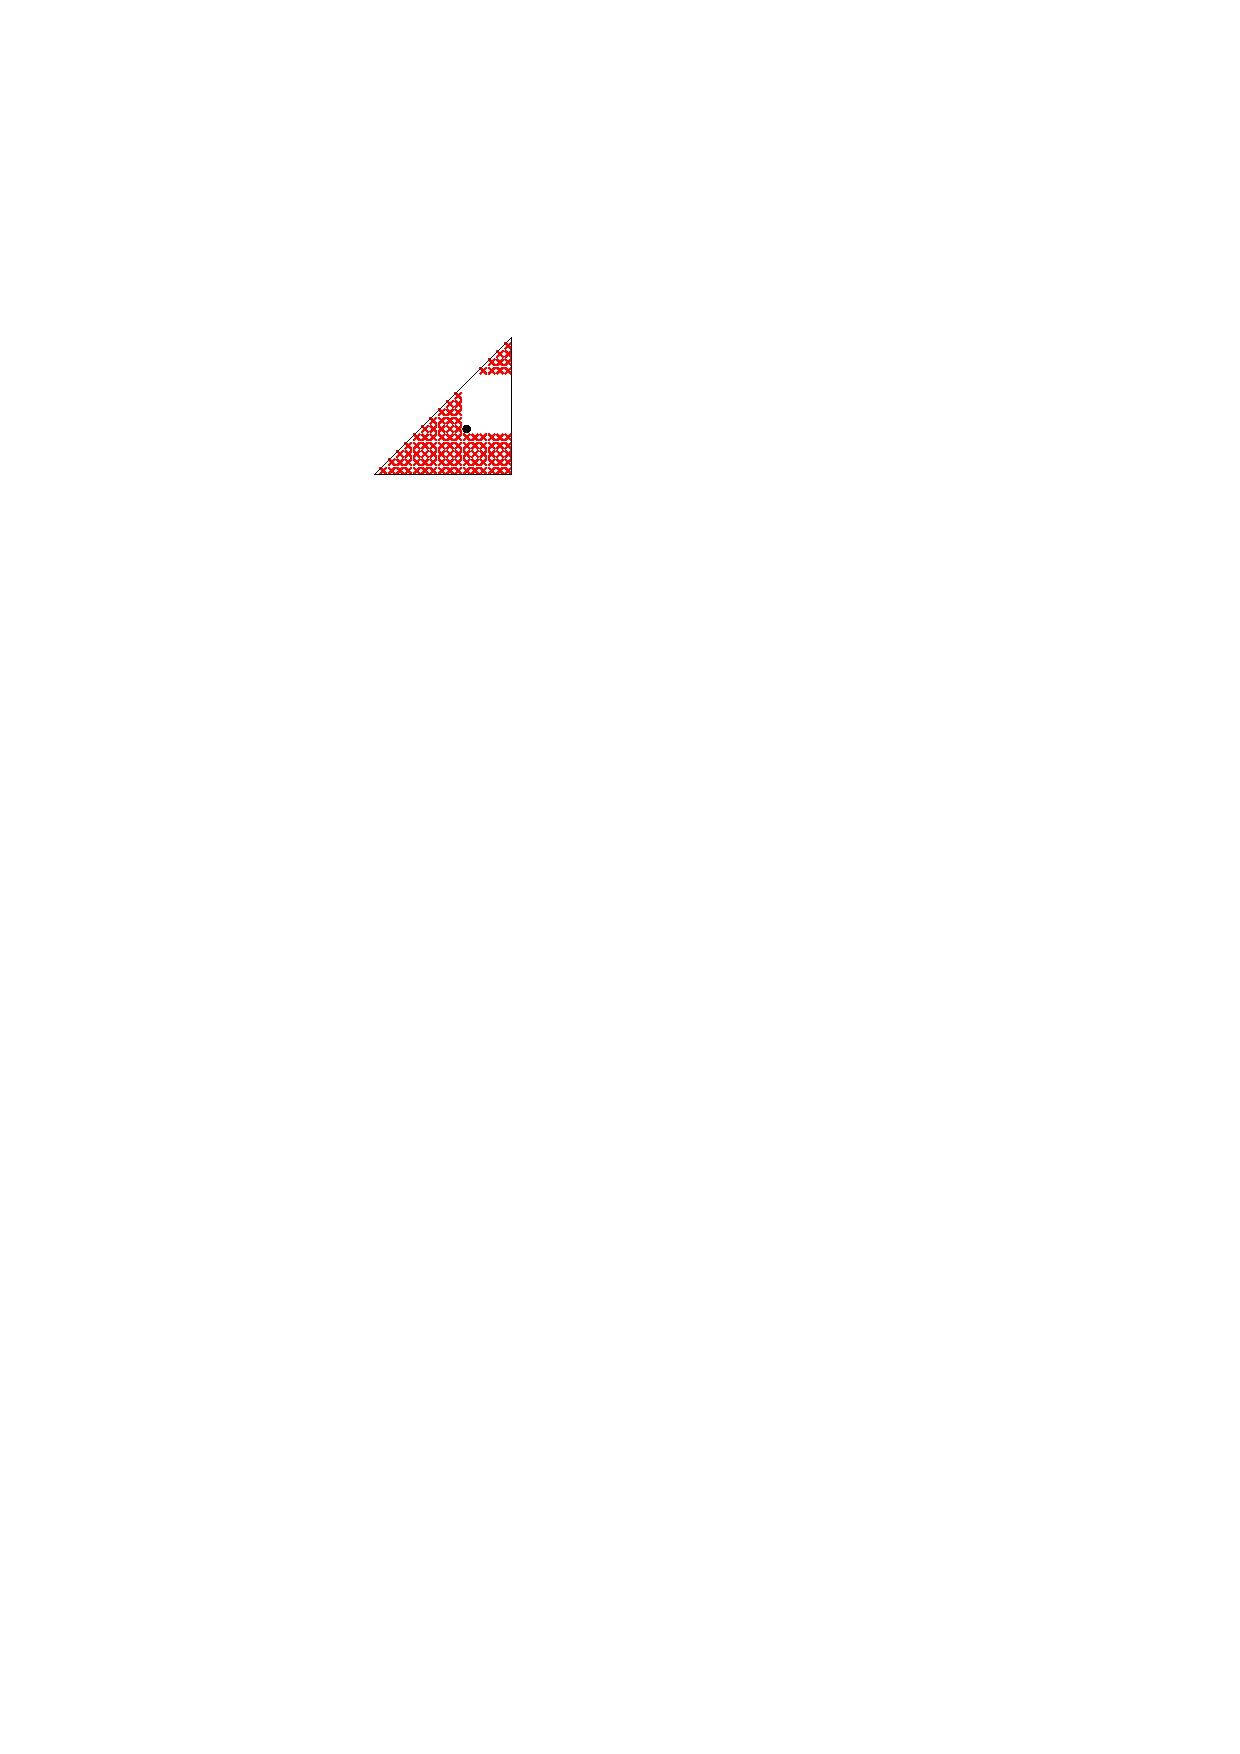
\includegraphics{figs/killers-9}
\end{center}
for which points are disallowed in subsequent rounds.  This rule ensures
that, after round $i$ any points chosen are either the topmost-rightmost
point in $Q_i$ or are above and to the right of this point.  Taken
together, these rules imply that
\[
    \sum_{i=1}^n|Q_i| \le 3n-2 \enspace ,
\]
Since the union of $Q_i$ is a non-decreasing point set (whose size is
therefore at most $2n-2$), and each $Q_i$ shares at most one point with
$Q_{i+1}$.  The bound $\ex(\ears, \swords, \bat,\nested)\in
O(n\log n)$ then follows from \lemref{top-bottom}.

\section{New Results}




% The following is the start of some bullshit argument, unless I can fix it.

%Earlier, we showed that the inclusion of the $\mariposa$ configuration in
%the set of excluded configurations, $X$, has no effect on the asymptotics
%of $\ex(n,X)$.  Here we show that a similar, though slightly weaker,
%result for the $\nested$ configuration.
%
%\begin{lem}
%  $\ex'(n,\{\taco,\bat\}\cup X) \in \Omega(\ex'(n,\{\taco\}\cup X)/\log n)$.
%\end{lem} 
%
%\begin{proof}[Proof Sketch]
%    Assume without loss of generality that $n$ is a power of 2 Partition
%    $Q$ into $O(\log n)$ \emph{layers}, where layer 0 contains
%    the \emph{square}, $L_0=\{(x,y)\in Q: x\ge n/2,\, y\le n/2\}$.
%    Subsequent layers are obtained by recursing on the two triangles in
%    $Q\setminus L_0$, so that $L_1$ contains two squares, $L_2$ contains
%    four squares, and so on.
%
%    Let $Q_1,\ldots,Q_n$ be a play of the dot-puzzle that achieves
%    $\ex'(n,\{\taco\}\cup X)$ while avoiding $\{\taco\}\cup X$
%    configurations.  Observe that, because we exclude $\taco$, the sets
%    $Q_i$ and $Q_j$ are disjoint for all $1\le i<j\le n$.
%
%    Then, for any layer $L_i$, the sets $Q_1\cap L_i,\ldots,Q_n\cap L_i$
%    avoid all configurations in $\{\taco\}\cup X$ as well as $\bat$
%    configurations.  By the pigeonhole principle, one of these layers,
%    say $L_i$, has size $\Omega(\ex'(n,\{\taco\}\cup X)/\log n)$.
%
%
%
%points that maximize
%\end{proof}
%
%is irrelevan
%

After this warm-up, and with the dot-puzzle view, we are ready to prove
some new results.  We begin with a collection of results on forbidding
the $\swords$ configuration.

\subsection{Forbidding Crossing Vertex-Disjoint Triangles}

In this section, we focus on the configuration $\swords$ and give
tight bounds bounds on $\ex'(n,\{\swords, Y\})$ for each of the
seven $Y\in\{\taco,\mariposa,\bat,\nested,\crossing,\ears,\david\}$.
Note that the bound $\ex'(n,\{\swords,\mariposa\})\in \Theta(n^2)$ is
immediate from bound $\ex(n,\{\swords\}\in\Theta(n^2)$ \cite{brass:turan}
and \lemref{xcup}.

In the following, we use the notation $\xmin(S)$ to denote the
minimum $x$-coordinate of any point in the point set $S$.  If $S$
is empty, then we define $\xmin(S)$ as $n+1$.  We define $\ymin(S)$,
$\xmax(S)$, and $\ymax(S)$ similarly, except that $\ymin(\emptyset)
= n$, $\ymax(\emptyset)=0$, and $\xmax(\emptyset)=1$.  For any
$X\subset\{\taco,\mariposa,\bat,\nested,\crossing,\ears,\swords,\david\}$
and any $S\subset Q$, we define $\survivors(X,S)$ to be the subset of
points in $Q$ that can still be played in the dot-puzzle game if the
points is $S$ have been played in previous rounds.

\begin{obs}\obslabel{swords-region}
  For any non-empty set $S\subset Q$, $\survivors(\{\swords\},S)$
  is contained in the union of a \emph{triangular region} $T=\{(x,y)\in
  Q: x\le \ymin(S)+1\}$, a \emph{rectangular region} $R=\{(x,y)\in Q:
  x\ge \xmax(S),\, y\ge \ymax(S)\}$, a \emph{vertical line} $V=\{(x,y)\in Q:
  x=\xmin(S)\}$ and a \emph{horizontal line} $H=\{(x,y)\in Q: y=\ymin(S)\}$.
\end{obs}

\obsref{swords-region} gives us a form of \emph{potential function}
that we can use.  We will apply it with $S=\bigcup_{j=1}^i Q_i$ so that as
rounds proceed, any time the value of $\xmax(S)$ or $\ymax(S)$ increase,
the size of the rectangle $R$ decreases. Any time the value of $\ymin(S)$
decreases, the size of the triangle $T$ decreases.  So that we can refer
to these point sets as they change, we let $S_i=\bigcup_{j=1}^i Q_i$ and
we define $T_i$, $R_i$, $V_i$, and $H_i$ as in \obsref{swords-region},
but with respect to the set $S=S_i$.

\begin{thm}\thmlabel{taco-swords}
  $\ex(n,\{\taco,\swords\}) \in O(n\log n)$.
\end{thm}

\begin{proof}
  We will directly bound $\sum_{i=1}^n |Q_i|$.  We begin by noting that,
  since we forbid $\taco$, the set of points in each $Q_i$ contains
  at most one point from each row and each column.  We will use this
  fact implicitly for the rest of the proof.

  Now, observe that if $Q_i$ contains $t_i\ge 2$ points in $T_i$, then
  $\ymin(S_{i+1}) \le \xmin(S_i)-t_i+2\}$.  This immediately
  implies that $\sum_{i=1}^n t_i \le 3n$.

  Similarly, if $Q_i$ contains $r_i\ge 1$ points in $R_i$, then
  $\ymax(S_{i+1})\ge \ymax(S_i)+r_i-1$.  This immediately
  implies that $\sum_{i=1}^n r_i\le 2n$.
  
  Finally, we observe that $Q_i$ contains at most one point each from
  $H_i$ and $V_i$, so
  \[
      \sum_{i=1}^{n}|Q_i| \le \sum_{i=1}^n(t_i+r_i+2) \le 7n \enspace .
  \]
  We have just shown that $\ex'(n,,\{\swords,\taco\})\in O(n)$,
  so the theorem follows from \lemref{top-bottom}.
\end{proof}

\begin{thm}\thmlabel{nested-swords}
  $\ex'(n,\{\nested,\swords\}) \in O(n)$.
\end{thm}

\begin{proof}
   The proof is similar to the proof of \thmref{swords-edgea}.
   The forbidden configuration $\nested$ implies that each set $Q_i$
   must be non-decreasing (see \figref{forbidden-color}a).
   We will use this fact implicitly for the rest of the proof.

   Now, if $Q_i$ contains $t_i$ points in $T_i$, then the fact
   that $Q_i$ is non-decreasing implies that $\ymin(S_{i+1})\le
   \ymin(S_i)-\lfloor t_i/2 \rfloor$.  This immediately implies that
   $\sum_{j=1}^n t_i \le 3n$.

   Similarly, if $Q_i$ contains $r_i\ge 1$ points in $R_i$, then the fact
   that $Q_i$ is non-decreasing means that
   \[
       \ymax(S_{i+1})+\xmax(S_{i+1}) 
             \ge \ymax(S_{i})+\xmax(S_{i}) + r_i - 1 \enspace .
   \]
   This immediately implies that $\sum_{j=1}^n r_i \le 3n$.

   To account for points of $Q_i$ on the vertical line $V_i$, we consider
   the lowest point of $\survivors(\{\swords\},Q_i)$ on  
   $V_i\setminus T_i\setminus R_i$ and denote the $y$-coordinate of this
   point by $y_i$.  If $V_i\setminus T_i\setminus R_i$ contains $v_i\ge
   1$ points of $Q_i$, then $y_{i+1}\ge y_i+v_i-1$.  This immediately
   implies that $\sum_{j=1}^n v_i \le 2n$.

   Accounting for points of $Q_i$ on the horizontal line $H_i$ is similar,
   but with respect to the left-most point of 
   $\survivors(\{\swords\},Q_i)$ in $H_i\setminus T_i\setminus R_i$.

   Summing everything, we find that
   $\ex'(n,\{\swords,\nested\})\le\sum_{j=1}^n |Q_i|\le 10n$, and
   we finish by applying \lemref{top-bottom}.
\end{proof}

\begin{thm}\thmlabel{crossing-swords}
  $\ex'(n,\{\crossing,\swords\}) \in O(n)$.
\end{thm}

\begin{proof}
  TODO. Similar to previous proof.
\end{proof}


\subsection{More Linear Upper Bounds}

\begin{thm}\thmlabel{taco-nested-crossing}
  $\ex'(n,\{\taco,\nested,\crossing\}) \in O(n)$.
\end{thm}

\begin{proof}
  Taking the union of the rules
  for $\taco$, $\nested$, and $\crossing$, we obtain the rule
  \begin{center}
     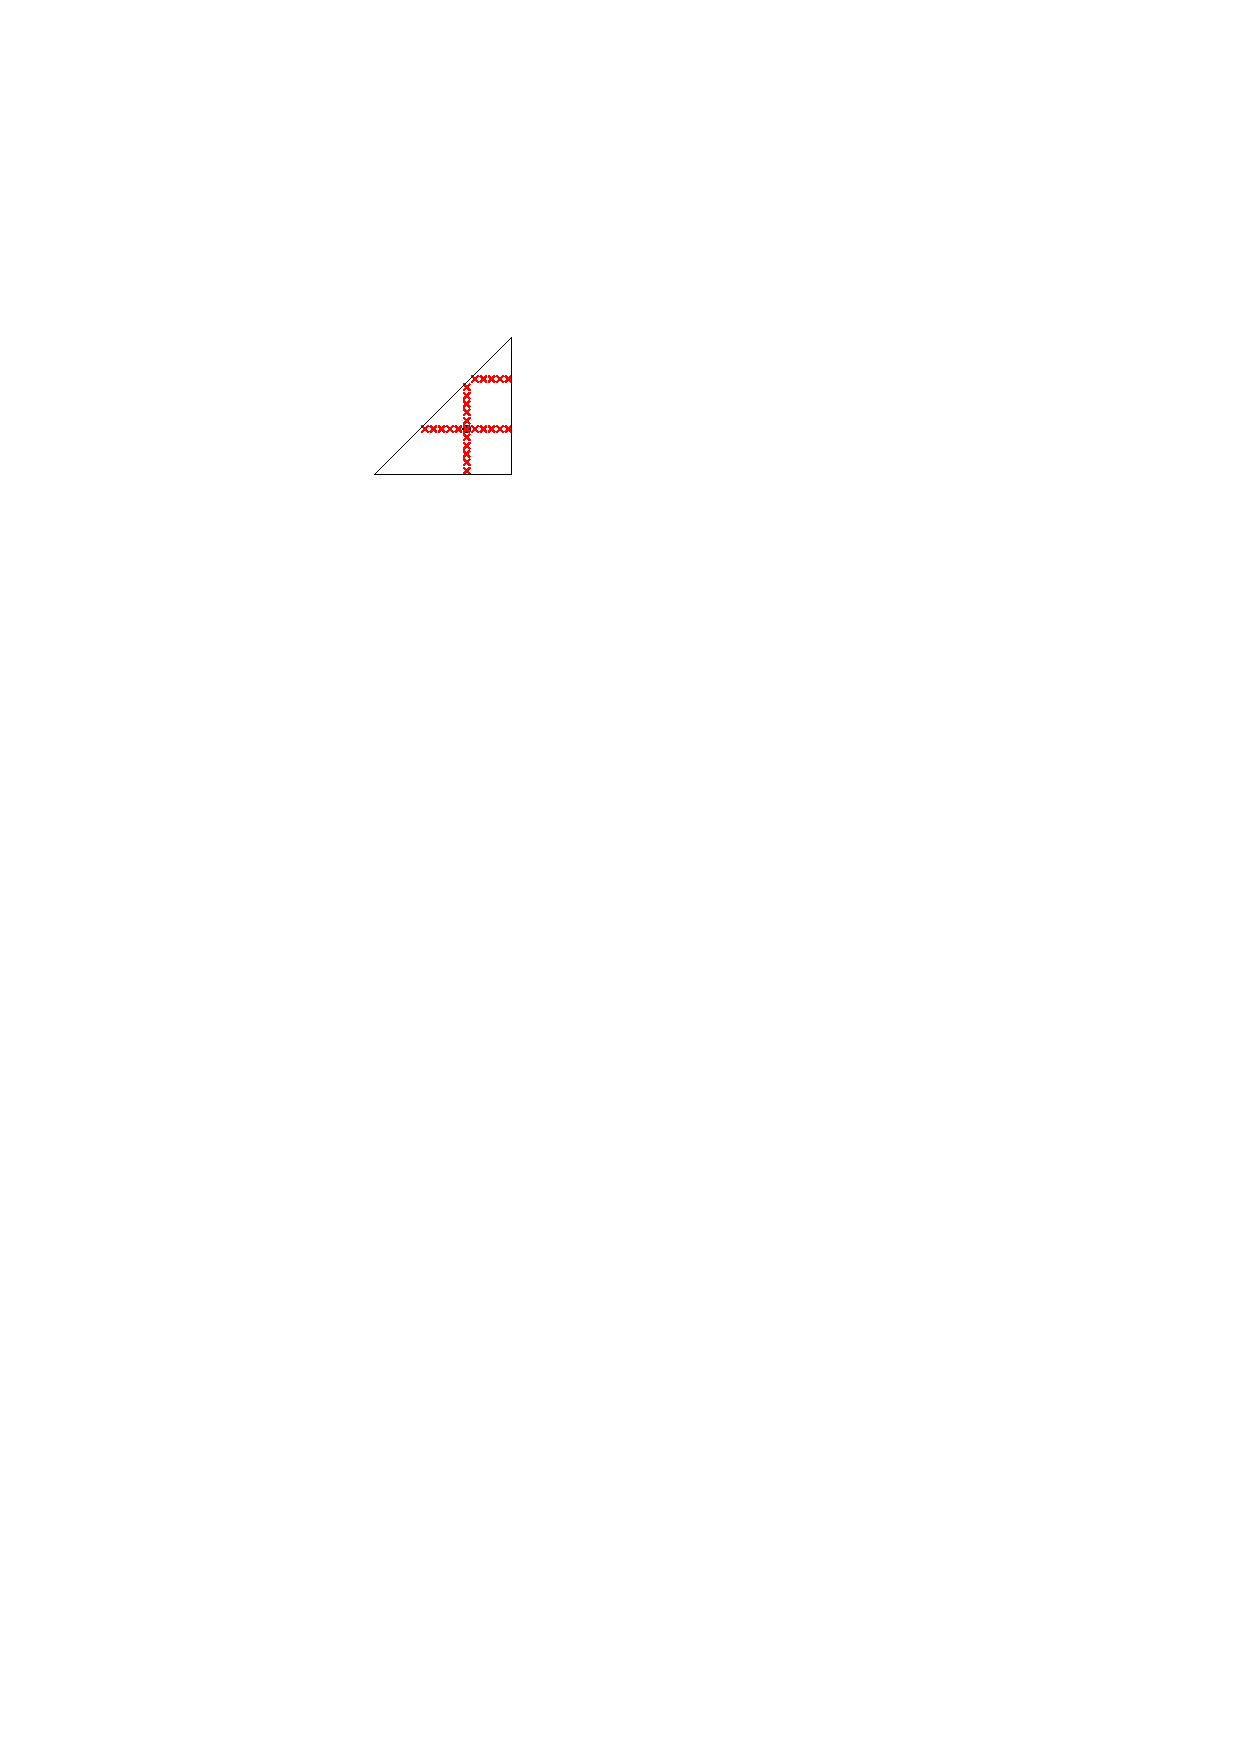
\includegraphics{figs/killers-10}
  \end{center}
  which ensures that during subsequent rounds we can not take a point
  from any column or row used in the previous round.  Since we forbid
  $\nested$, we know that the set of points taken during each round
  is non-decreasing.

  Imagine scanning the points in $Q_i$ in non-decreasing order.  Combining
  the two preceding observations, we see that each point we scan is in
  a row and column not used before in $Q_1,\ldots,Q_{i-1}$ and it is
  on a row or a column that has not appeared before in the scan order.
  Thus, each point of $Q_i$ that we scan kills one row and/or one column
  so that this row/column can not be used in $Q_{i+1},\ldots,Q_n$.  Therefore,
  $\sum_{j=1}^n |Q_i| \le 2n-3$.
\end{proof}



\begin{thm}\thmlabel{nested-crossing-ears}
  $\ex'(n,\{\nested,\crossing,\ears\})\in O(n)$.
\end{thm}

\begin{proof}
  First observe that the rules for $\nested$ imply that each $Q_i$
  is a non-decreasing sequence of points.

  Next, observe that if $Q_i$ contains $k>1$ points in a single column
  (or row), then each of the $k$ rows (or columns) containing one of these
  points is killed. $Q_{i+1},\ldots,Q_n$ can not contain any points in
  these rows (or columns).  Therefore, when summing $\sum_{i=1}^n |Q_i|$,
  the contribution of points that are not alone in their row or column
  is at most $n$.  We therefore assume that each $Q_i$ contains at most
  one point from each row and column, which now implies that each $Q_i$
  is an increasing sequence of points.

  Now, because of the rules for $\crossing$, this increasing
  requirement is quite strong. In particular, if we consider the last
  (highest-righmost) point of $Q_i$, then it must be placed so that the
  set of points killed by its $\ears$-region contains all points in $Q_i$
  except itself and the second-last point of $Q_i$.

  To summarize, each row and column of $Q$ contributes at most point to
  the set
  $S=\bigcup_{i=1}^n Q_i$, so $|S|\le n$.  However, $Q_1$ eliminates $|Q_1|-2$ elements of from $S$ and, in round $i$, $Q_i$ eliminates an additional $|Q_{i}|-2$ elements from $S$.  Therefore,
  \[
        n\ge |S| \ge \sum_{i=1}^n (|Q_i|-2) \enspace ,
  \] 
  and we conclude that $\sum_{i=1}^n|Q_i| \le 3n$.
\end{proof}


Our final two upper bounds depend on a simple lemma about forbidden
configurations of points:

\begin{lem}\lemlabel{forbidden}
   Let $S$ be a subset of the $\{1,\ldots,n\}^2$ such with no three
   points $a=(x_0,y_0)$, $b=(x_0,y_1)$, and $c=(x_1,y_1)$ with $y_0<y_1$
   and $x_0<x_1$.  Then $|S|\le 2n$.
\end{lem}

\begin{proof}
   If we remove the rightmost point from each row of $S$, then each
   column in what remains of $S$ contains at most one point. Otherwise we
   could take $a$ to be the lowest point in a column, $b$ to the highest
   point in the same column, and $c$ to be the missing rightmost point
   in $b$'s row.
\end{proof}

\begin{thm}\thmlabel{taco-nested-david}
  $\ex'(n,\{\taco,\nested,\david\})\in O(n)$.
\end{thm}

\begin{proof}
  Let $S=\bigcup_{i=1}^n Q_i$ be the set of points played in a solution
  to the resulting dot-puzzle.  Note that, by the inclusion of $\taco$,
  each element of $S$ appears in exactly one $Q_i$, so $|S|=\sum_{i=1}^n
  |Q_i|$ is the quantity we are interested in bounding.

  Next, we observe that $S$ does not contain any three points
  $a=(x_0,y_0)$, $b=(x_0,y_1)$, and $c=(x_1,y_1)$ with $y_0<y_1$
  and $x_0<x_1$.  This is because the rules for $\taco$ and $\nested$
  imply that $a$ would have to have been played in a round before $b$,
  and that $b$ would have to have been played in a round before $c$.
  But then the rule for $\david$ implies that $c$ would have to appear
  in a round before $a$.  Applying \lemref{forbidden} then implies that
  $|S|\le 2n$.
\end{proof}


\begin{thm}\thmlabel{nested-bat-david}
  $\ex'(n,\{\nested,\bat,\david\})\in O(n)$.
\end{thm}

\begin{proof}
  Consider the set $Q_i$ played during some round $i$.  The rules for
  $\nested$ imply that $Q_i$ is non-decreasing.  The rule for $\bat$
  implies that $Q_i$ is contained in the $\david$-region, $R_i$, of the
  lowest-leftmost point in $Q_i$.  Indeed, all of $Q_i$ except its
  leftmost row and column is in this david region.

  Suppose we remove the leftmost point in each row of $Q_i$.  For each
  such point $p\in R_i$, the entire row containing $p$ is then killed
  and can never be played again.  The remaining points are in the first
  column of $Q_i$ and all but two of these (the topmost and bottommost)
  kill an entire row that can never be played again.  This means that
  the total number of points removed this way is not more $3n$ (one
  charged to each row and two charged to each round).  Since $Q_i$ was
  originally non-decreasing, the removal of these points ensures that
  each column contains at most one point of $Q_i$

  Now we let $S=\bigcup_{i=1}^n Q_i$.  We claim that $S$ fulfills the
  requirements of \lemref{forbidden}.  To see why this is so, note that
  if two points $a$ and $b$ of $S$ are in the same column then they
  must have been played in different rounds.  Assume $b$ is above $a$,
  which implies that $b$ was played in a later round than $a$.  Then, if
  there is some point $c$ to the right of $b$, then $c$ must have played
  during the same round as $b$ or later.  But this implies that $c$ was
  played in a later round than $a$, which is not possible, since $c$ is in
  $a$'s $\david$-region.  Therefore, by \lemref{forbidden}, $|S|\le 2n$.

  All that remains is to account for points in $S$ that are played
  multiple times.  In each $Q_i$ there are at most two points that can
  be played in subsequent rounds; the topmost point in the leftmost
  column and the rightmost point in the bottommest row.  We charge each
  occurrence of such repeated points to the rounds in which they are
  the topmost point in the leftmost column and/or the rightmost point
  in the bottommost row.  In this way, each round is charged for at
  most two such points and the total contribution of these points to
  $\sum_{i=1}^n |Q_i|$ is at most $2n$.

  In total, we obtain an upper bound of $7n$ on $\sum_{i=1}^n |Q_i|$.
\end{proof}





\subsection{Montone Matrices, Tripod Packing, and 2-Comparable Sets}

Determining the asymptotics of $\ex(n,\{\taco,\nested\})$ was given explicitly as open problem in the conclusion of Bra\ss's paper.  We spent more than a year work on this problem and this work included computer searches for solutions for small values of $n$.  Using the results of these computer searches in the Online Encyclopedia of Integer Sequences, we discovered that this problem is (asymptotically) equivalent to several other known problems.

\begin{enumerate}
  \item Monotone matrices
  \item Tripod packing
  \item 2-comparable sets of triples.
\end{enumerate}

One observation we have on this problem is that $\ex'(n,\{\taco,\nested\})=\Theta(\ex'(n,\{\taco,\nested,\bat,\ears\})$.  This comes from the fact that any solution\ldots

\subsection{Lower Bounds}

Finally, we clean up with some lower bound constructions.  In each
case, a matching upper bound follows from one of the results in Bra\ss
\cite{brass:turan}.  We start with very large sets of triangles, all of
which pairwise cross.

\begin{thm}\thmlabel{pairwise-crossing}
   $\ex(n,\{\ears,\bat,\mariposa\})=\Theta(n^3)$
\end{thm}

\begin{proof}
  The $O(n^3)$ upper bound is immediate.  For the lower bound,
  partition the points of the convex $n$-gon into three contiguous
  sets, $A$, $B$, and $C$, each of size $\lfloor n/3\rfloor$ or
  $\lceil n/3\rceil$, as appropriate.  Consider the set, $S$, of all
  triangles having one vertex in each of $A$, $B$, and $C$. It is easy
  to check that any two triangles in $S$ have a pair of edges that
  cross, thus they do not form any of \ears, \bat, or \mariposa.
  Furthermore, $|S|\ge \lfloor n/3\rfloor^3=\Omega(n^3)$, so
  $\ex(n,\{\ears,\bat,\mariposa\})=\Omega(n^3)$.
\end{proof}

Next we present a series of fairly easy $\Omega(n^2)$ lower bound
constructions.

\begin{thm}\thmlabel{taco-david-bat-ears}
$\ex(n,\{\taco,\david,\crossing,\bat,\ears\})\in\Theta(n^2)$.
\end{thm}

\begin{proof}
We set $Q_i$ to be all the points of $\{n/2,\ldots,n\}^2$ on the line $y=n-x-i$.
\end{proof}

\begin{thm}\thmlabel{swords-bat-ears-david}
  $\ex(n,\{\swords,\bat,\ears,\david\}) \in \Theta(n^2)$.
\end{thm}

\begin{proof}
   We set $Q_1=\{(x,y)\in Q: x>n/2, y<n/2\}$ and
   set $Q_2=Q_3=\cdots Q_n=\emptyset$.
\end{proof}

\begin{thm}\thmlabel{nested-ears-david}
  $\ex(n,\{\nested,\ears,\david\}) \in \Theta(n^2)$.
\end{thm}

\begin{proof}
   Keep taking the bottom row.
\end{proof}

\begin{thm}\thmlabel{david-nested-crossing}
  $\ex(n,\{\david,\nested,\crossing\}) \in \Theta(n^2)$.
\end{thm}

\begin{proof}
   We repeatedly take points on the diagonal.
\end{proof}

\begin{thm}\thmlabel{bat-nested-ears}
  $\ex(n,\{\bat,\nested,\ears\}) \in \Theta(n^2)$.
\end{thm}

\begin{proof}
   We repeatedly take points on the diagonal inside the square.
\end{proof}



\section*{Acknowledgement}

Some of this work was carried out at the e Fourth Annual Workshop on
Geometry and Graphs, held at the Bellairs Research Institute in Barbados,
March 6--11, 2016. The authors are grateful to the organizers and to
the participants of this workshop for providing a stimulating working
environment.


\bibliographystyle{plain}
\bibliography{turan}

\end{document}


